\documentclass[10pt]{beamer}

\usetheme{Frankfurt}
\useoutertheme{default}
\setbeamertemplate{footline}[page number]
\setbeamertemplate{navigation symbols}{} 
\setbeamertemplate{caption}{\raggedright\insertcaption\par}

%%% Работа с русским языком
\usepackage{cmap}					% поиск в PDF
\usepackage[T2A]{fontenc}			% кодировка
\usepackage[utf8]{inputenc}			% кодировка исходного текста
\usepackage[english,russian]{babel}	% локализация и переносы
\usepackage{indentfirst}
\frenchspacing

\usepackage{subfigure}

%%% Дополнительная работа с математикой
\usepackage{amsmath,amsfonts,amssymb,amsthm,mathtools} % AMS
\usepackage{icomma} % "Умная" запятая: $0,2$ --- число, $0, 2$ --- перечисление

%%% Работа с картинками
\usepackage{graphicx}  % Для вставки рисунков
\usepackage{wrapfig} % Обтекание рисунков текстом
\usepackage{subfigure}

%%% Работа с таблицами
\usepackage{array,tabularx,tabulary,booktabs} % Дополнительная работа с таблицами
\usepackage{longtable}  % Длинные таблицы
\usepackage{multirow} % Слияние строк в таблице

%%% Программирование
\usepackage{etoolbox} % логические операторы


\usepackage{setspace} % Интерлиньяж
%\onehalfspacing % Интерлиньяж 1.5
%\doublespacing % Интерлиньяж 2
%\singlespacing % Интерлиньяж 1

\usepackage{lastpage} % Узнать, сколько всего страниц в документе.

\usepackage{soul} % Модификаторы начертания

\usepackage{tikz} % Работа с графикой
\usepackage{pgfplots}
\usepackage{pgfplotstable}

\renewcommand{\phi}{\varphi}
\renewcommand{\epsilon}{\varepsilon}

\newcommand{\delayV}[1]{\overset{\leftarrow}{\textbf{x}}_{#1}}
\newcommand{\delayM}[1]{\overset{\leftarrow}{\mathbf{X}}_{#1}}

\theoremstyle{definition}
\newtheorem*{Def}{Определение}

\title{Тензорная декомпозиция и прогноз для набора временных рядов}
\author{Сёмкин Кирилл}

\institute[MIPT]{Московский физико-технический институт \\ Кафедра интеллектуальных систем}

\date[2024]{\textit{Научный руководитель}: д.ф.-м.н. Стрижов Вадим Викторович \\ 2024}

\begin{document}
	
	\begin{frame}[c]
		\titlepage
	\end{frame}

	\begin{frame}{Мотивация}
		
		\begin{alertblock}{Проблема}
			Обработка многомерных временных рядов влечёт необходимость учёта взаимосвязей сигналов. Нейросетевые и статистические подходы имеют большое количество параметров, и требуют изощрённых процедур обучения. При этом они не предлагают способа построения декомпозиции.
		\end{alertblock}
		
		\begin{block}{Цель}
			Предложить метод, позволяющий выделить общую для набора сигналов структуру. На её основании произвести разложение каждого сигнала на компоненты. Найти способ построения прогноза.
		\end{block}
		
		\begin{exampleblock}{Решение}
			\textbf{tSSA} = модель собственного пространства сигнала + тензорное представление данных + CPD
		\end{exampleblock}
		
	\end{frame}	
	
	\begin{frame}{Модель порождения наблюдаемых сигналов}
		
		\emph{Динамическая система} в дискретном времени:
		
		\begin{equation*}
			\begin{cases}
				\textbf{y}(t + 1) = f(\textbf{y}(t)), \ t \in \mathbb{N} \\
				\textbf{y}(0) = \textbf{y}_0
			\end{cases}
		\end{equation*}
		
		$ \textbf{y} \in X $, где $ X $ --- гладкое многообразие большой размерности. 
		
		Конкретная траектория этой системы \emph{порождает} наблюдаемые ряды через некое многомерное отображение $ \boldsymbol{\phi}: X \to \mathbb{R}^m $:
		
		\begin{equation*}
			\boldsymbol{\phi}\bigl(\textbf{y}(t)\bigl) = \textbf{x}_t \Leftrightarrow \begin{cases}
				\phi_1\bigl(\textbf{y}(t)\bigl) = x_1(t) \\
				\ldots \\
				\phi_m\bigl(\textbf{y}(t)\bigl) = x_m(t) \\
			\end{cases}
		\end{equation*}
		
	\end{frame}
	
	\begin{frame}{Низкоразмерное представление динамической системы}
		
		Траектории $ \textbf{y}(t) $ лежат в многообразии $ M \subset X $ размерности  меньшей, чем у $ X $. Ставится задача поиска вложения (embedding) $ M $ в $ \mathbb{R}^{L} $ для некоторого $ L $ и нахождения базиса в образе этого вложения.
		
		\begin{figure}[h]
			\centering
			
			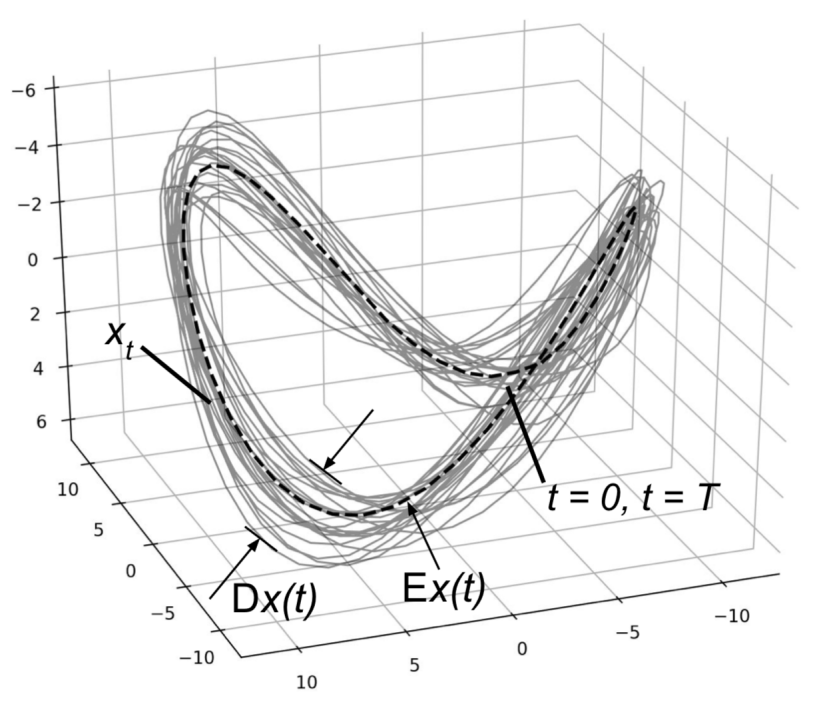
\includegraphics[width=0.6\textheight, keepaspectratio]{img/dynamic_system_example.png}
			\caption{Динамическая система собственной размерности < 3}
			
		\end{figure}
		
	\end{frame}
	
	\begin{frame}{Решение для одного сигнала}
		
		\begin{theorem}[Такенс]
			Искомое вложение даётся построением соответствующего вектора задержки 
			
			\begin{equation*}
				\textbf{y}(t) \xrightarrow{emb} \begin{pmatrix}
					\boldsymbol{\phi} \circ f^{t - L + 1}\bigl(\textbf{y}(t)\bigl) \\
					\vdots \\
					\boldsymbol{\phi} \circ f\bigl(\textbf{y}(t)\bigl) \\
					\boldsymbol{\phi} \circ \textbf{y}(t)
				\end{pmatrix} = \begin{pmatrix}
					x(t - L + 1) \\
					\vdots \\
					x(t - 1) \\
					x(t)
				\end{pmatrix} = \delayV{t} \in \mathbb{R}^L
			\end{equation*}
			
		\end{theorem}
		
		Полученное пространство вложения $ \text{Lin}\bigl(\{\delayV{t}\}\bigl) $ есть \emph{собственное пространство сигнала} $ x(t) $.
		
		C помощью разложения \emph{траекторной матрицы} $ \mathbf{H}_x = [ \delayV{1} \ldots  \delayV{N - L + 1}]. $ выделяем базис. Далее можем декомпозировать и строить прогноз (SSA). 
	
	\end{frame}
	
	\begin{frame}{Построение траекторного тензора}
		
		Упакуем векторы задержек всех рядов в \emph{матрицы задержек} $ ( \delayV{1_t} \ldots \delayV{m_t} ) := \delayM{t} $. Состыкуем их в \emph{траекторный тензор} $ \textbf{T} $.
		
		\begin{figure}[h]
			\centering
			\subfigure{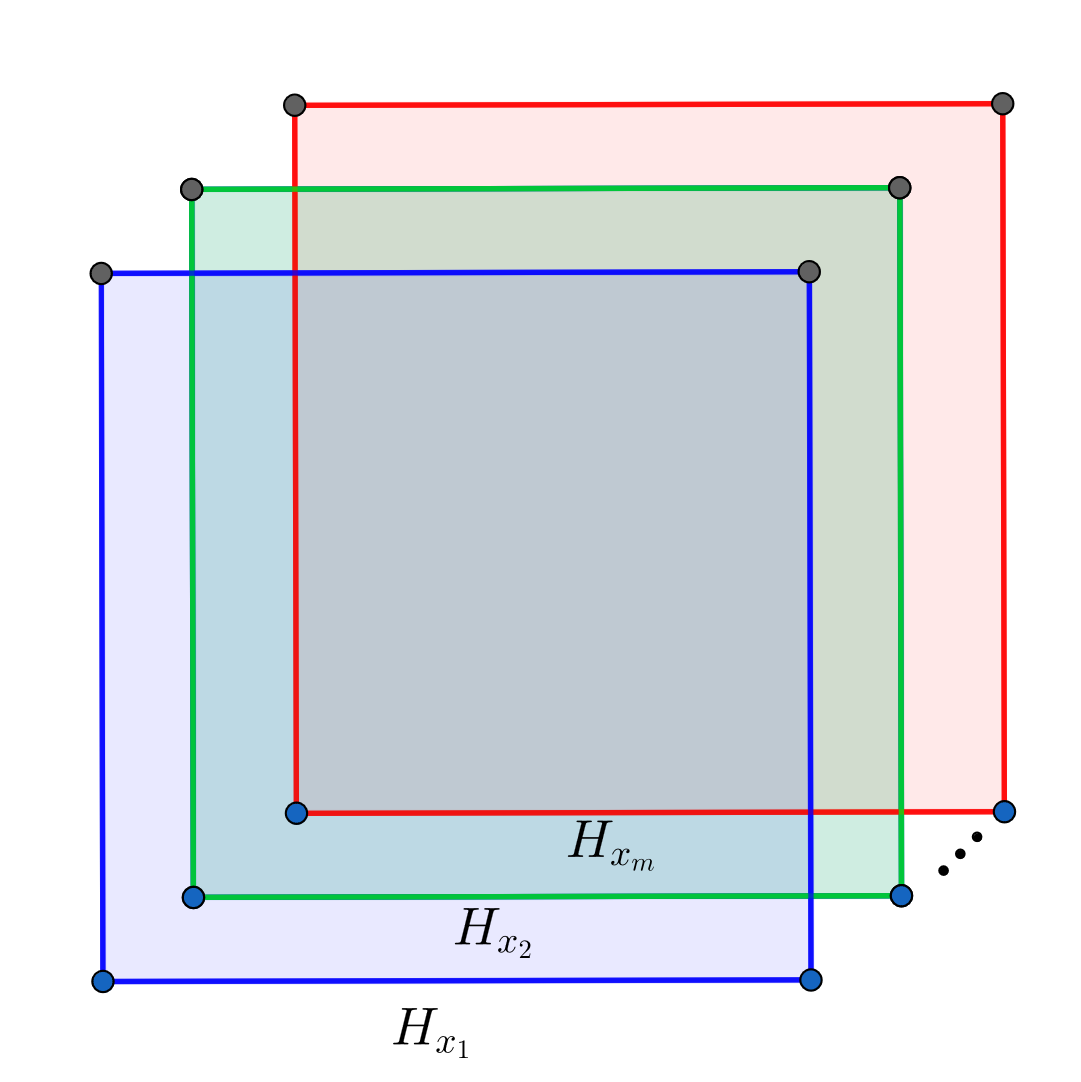
\includegraphics[width=0.4\textwidth, keepaspectratio]{img/Trajectory_Tensor_1}}
			\subfigure{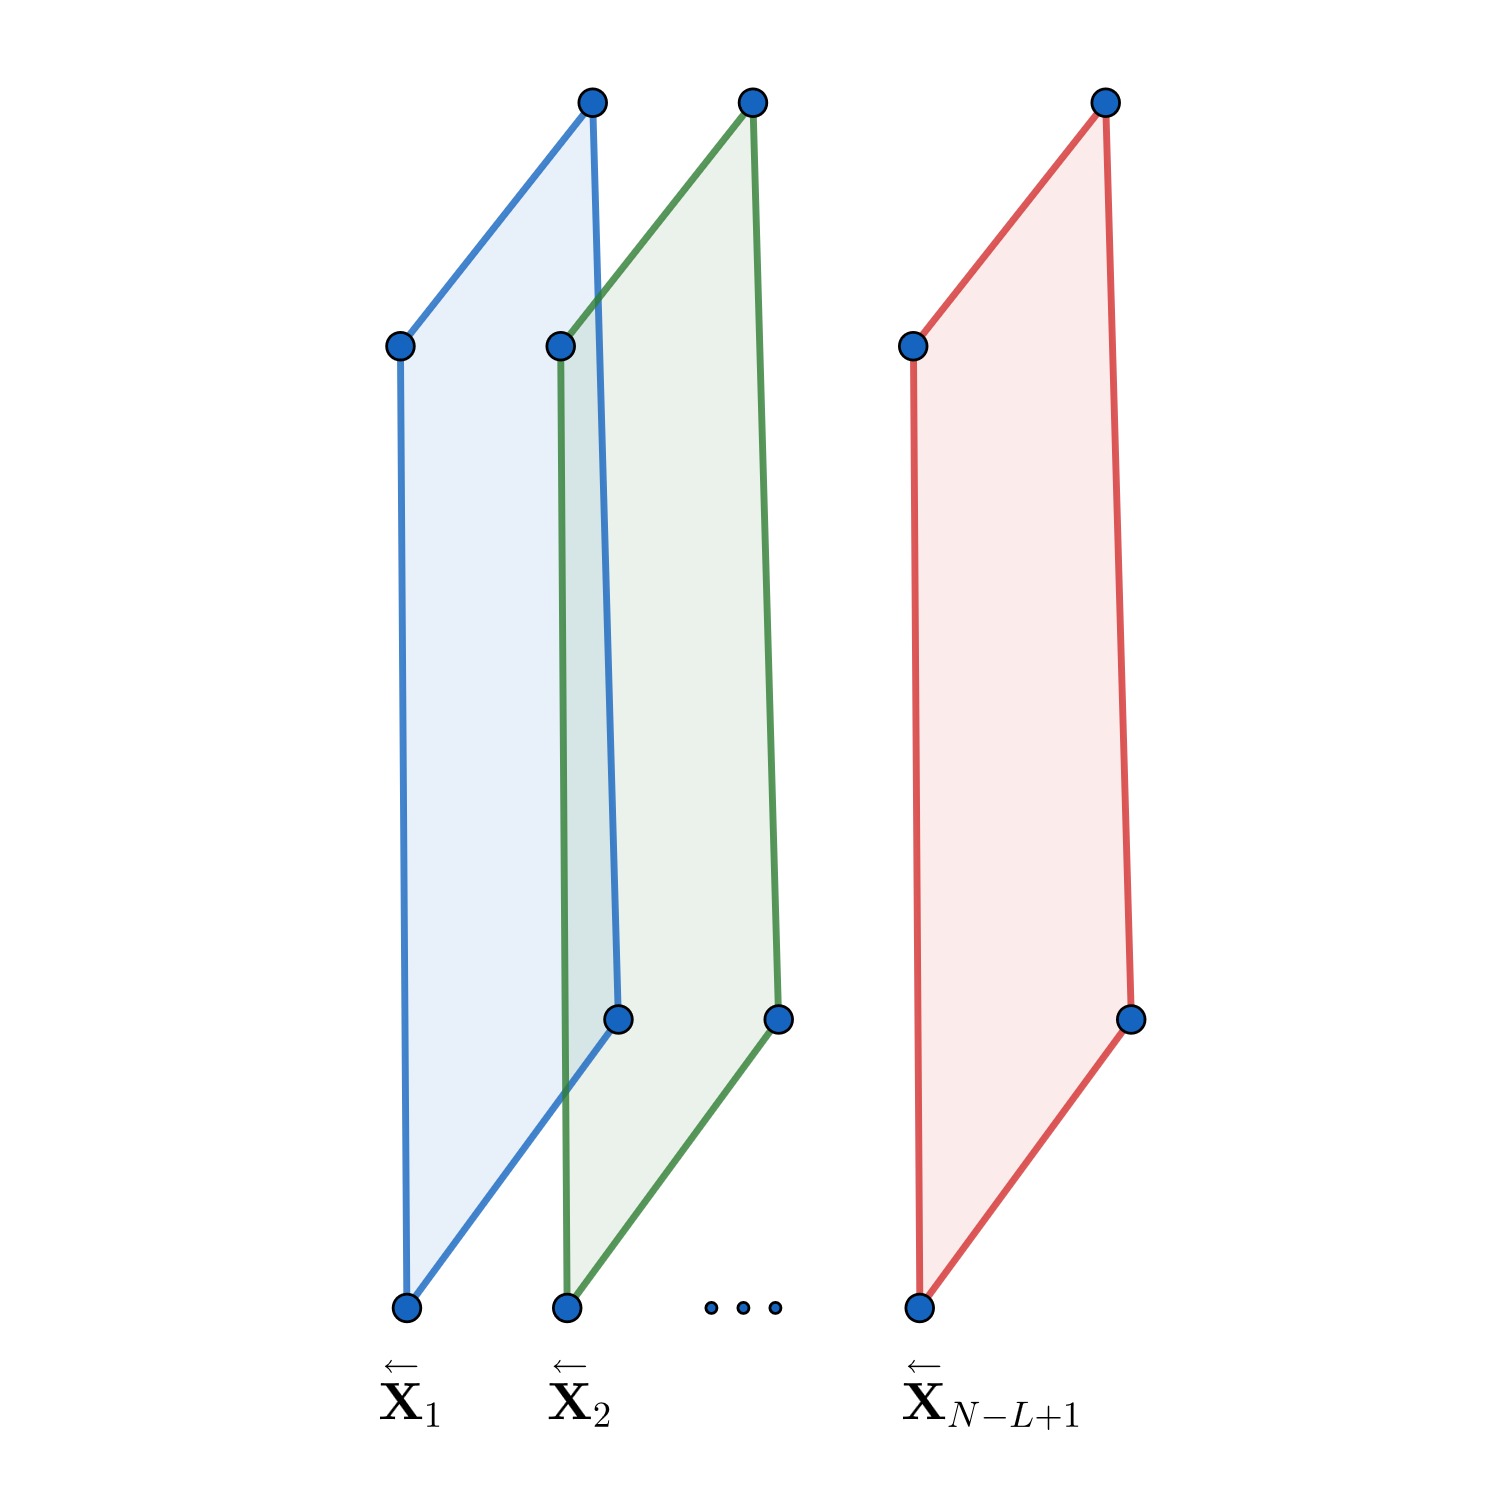
\includegraphics[width=0.4\textwidth, keepaspectratio]{img/Trajectory_Tensor_2}}
			
			\caption{Два вида на $ \textbf{T} $. Слева --- в виде набора траекторных матриц сигналов. Справа --- в виде набора матриц задержки.}\label{pic:traj_tensor}
		\end{figure}
		
	\end{frame}
	
	\begin{frame}{Решение для нескольких сигналов}
		
		Применим \textit{CP-разложение} к траекторному тензору и рассмотрим каждое его сечение по третьему измерению:
		
		\begin{equation*}\label{eq:tSSA_decomp}
			\textbf{T} = \sum\limits_{i = 1}^{r} \mathbf{a}_i \otimes \mathbf{b}_i \otimes \mathbf{c}_i \Leftrightarrow \begin{cases}
				\mathbf{H}_{x_1} = \sum\limits^{r} \boldsymbol{\sigma}_{x_1}(i) \cdot \mathbf{a}_i  \mathbf{b}_i^{\mathsf{T}}  \\
				\mathbf{H}_{x_2} = \sum\limits^{r} \boldsymbol{\sigma}_{x_2}(i) \cdot \mathbf{a}_i  \mathbf{b}_i^{\mathsf{T}} \\
				\ldots \\
				\mathbf{H}_{x_m} = \sum\limits^{r} \boldsymbol{\sigma}_{x_m}(i) \cdot \mathbf{a}_i  \mathbf{b}_i^{\mathsf{T}} 
			\end{cases}
		\end{equation*}
		
		Получили разложение траекторных матриц сигналов по \emph{общему базису} $ \{\mathbf{a}_i\}_{i = 1}^r $. Связь рядов определяют $ \boldsymbol{\sigma}_{x_k} $, имеющие смысл сингулярных чисел.
		
	\end{frame}
	
	\begin{frame}{Аддитивное разложение сигналов}
		
		\textit{Принцип построения}: декомпозиция траекторной матрицы $ \mathbf{H}_{x_k} $ определяет декомпозицию временного ряда $ x_k(t) $.
		
		Факторы разложения $ \mathbf{H}_{x_k} $ разбиваем на группы и \emph{ганкелизуем} --- усредняем матрицы по антидиагоналям.
		
		\begin{multline*}
			\mathbf{H}_{x_k} = \sum\limits_{i = 1}^{r} \boldsymbol{\sigma}_{x_k}(i) \cdot \mathbf{a}_i  \mathbf{b}_i^{\mathsf{T}} = \sum\limits_{i \in \mathbb{I}_1} \boldsymbol{\sigma}_{x_k}(i) \cdot \mathbf{a}_i  \mathbf{b}_i^{\mathsf{T}} + \ldots + \sum\limits_{i \in \mathbb{I}_s} \boldsymbol{\sigma}_{x_k}(i) \cdot \mathbf{a}_i  \mathbf{b}_i^{\mathsf{T}} = \\ = C_1 + \ldots + C_s = \text{Hankel}(C_1) + \ldots + \text{Hankel}(C_s)  \Leftrightarrow x_k(t) = c_1(t) + \ldots c_s(t)
		\end{multline*}
		
		\begin{exampleblock}{Наблюдение}
			Чем ближе по структуре $ C_i $ похожи на ганкелевы, тем более естественно построение итогового разложения. 
		\end{exampleblock}
		
	\end{frame}
	
	\begin{frame}{Оптимальная декомпозиция}
		
		Обозначим невязку $ H_i = \boldsymbol{\sigma}_{x_k}(i) \cdot \mathbf{a}_i  \mathbf{b}_i^{\mathsf{T}} - Hankel(\boldsymbol{\sigma}_{x_k}(i) \cdot \mathbf{a}_i  \mathbf{b}_i^{\mathsf{T}}) $. Тогда из предыдущего выражения следует:
		
		\begin{equation*}
			H_1 + \ldots + H_r = 0
		\end{equation*}
			
		Разбиваем на две группы. В каждой хотя бы две невязки, суммирующиеся в ноль. Условие оптимальной декомпозиции:
			
		\begin{equation*}
				\begin{cases*}
					\sum\limits_{j = 1}^{r - 1} \beta_j H_j = 0 \\
					\beta_j \in \{0, 1\}, \ \forall j \in 1, \ldots, r \\
					\sum\limits_{i = 1}^{r - 1} \beta_j \ge 2
				\end{cases*} \to
				\begin{cases*}
					\lVert \Lambda \boldsymbol{\beta} \rVert \to \underset{\boldsymbol{\beta}}{\min} \\
					\beta_j \in \{0, 1\}, \ \forall j \in 1, \ldots, r \\
					\sum\limits_{i = 1}^{r - 1} \beta_j \ge 2
				\end{cases*}
		\end{equation*}
		
		Имеем задачу наименьших квадратов с целочисленными ограничениями (ILS), которая является NP-сложной.
		
	\end{frame}
	
	\begin{frame}{Построение среднего прогноза}
		
		Базис в пространстве векторов задержек сигнала даётся как $ \text{Lin}(\{\mathbf{a}_i\}) \Leftrightarrow A = [\mathbf{a}_1 \ldots \mathbf{a}_r] $. 
		
		Прогноз на один шаг вперёд сводится к решению частично неизвестной СЛАУ:
		
		\begin{gather*}\label{eq:main_pred_for_A}
			\delayV{N + 1} = A \boldsymbol{\lambda} \Leftrightarrow \begin{cases}
				\mathbf{x}_{kn} = A_{kn} \boldsymbol{\lambda}  \\
				x(N + 1) = \mathbf{a}_{pr}^{\mathsf{T}} \boldsymbol{\lambda}
			\end{cases}, \text{ где } \\
			A = \left( \dfrac{A_{kn}}{\mathbf{a}_{pr}^{\mathsf{T}}} \right) \nonumber \\
			\delayV{N + 1} = (\mathbf{x}_{kn}, \  x(N + 1))^{\mathsf{T}} \nonumber
		\end{gather*}
		
		Система переопределена, решение даётся в смысле наименьших квадратов:
		
		\begin{equation*}
			x(N + 1) = \mathbf{a}_{pr}^{\mathsf{T}} (A_{kn}^T A_{kn})^{-1} A_{kn}^T \mathbf{x}_{kn}
		\end{equation*}
		
		% TODO: сказать здесь о авторегрессии
		
	\end{frame}
	
	\begin{frame}{Постановка эксперимента}
		
		\textit{Рассматриваемые ряды}:
		
		 \begin{enumerate}
		 	\item план выработки электричества на день и цена его производства
		 	\item показания акселерометра и гироскопа (ходьба)
		 \end{enumerate}
		 
		 \textit{Модели для сравнения}: mSSA, VAR, RNN.
		 
		 \textit{Метрики}: 
		 
		 \begin{enumerate}
		 	\item Прогнозирование: MSE, MAPE
		 	\item Декомпозиция: AHE, RHE
		 \end{enumerate}
		 
		 \begin{figure}[h]
		 	\centering
		 	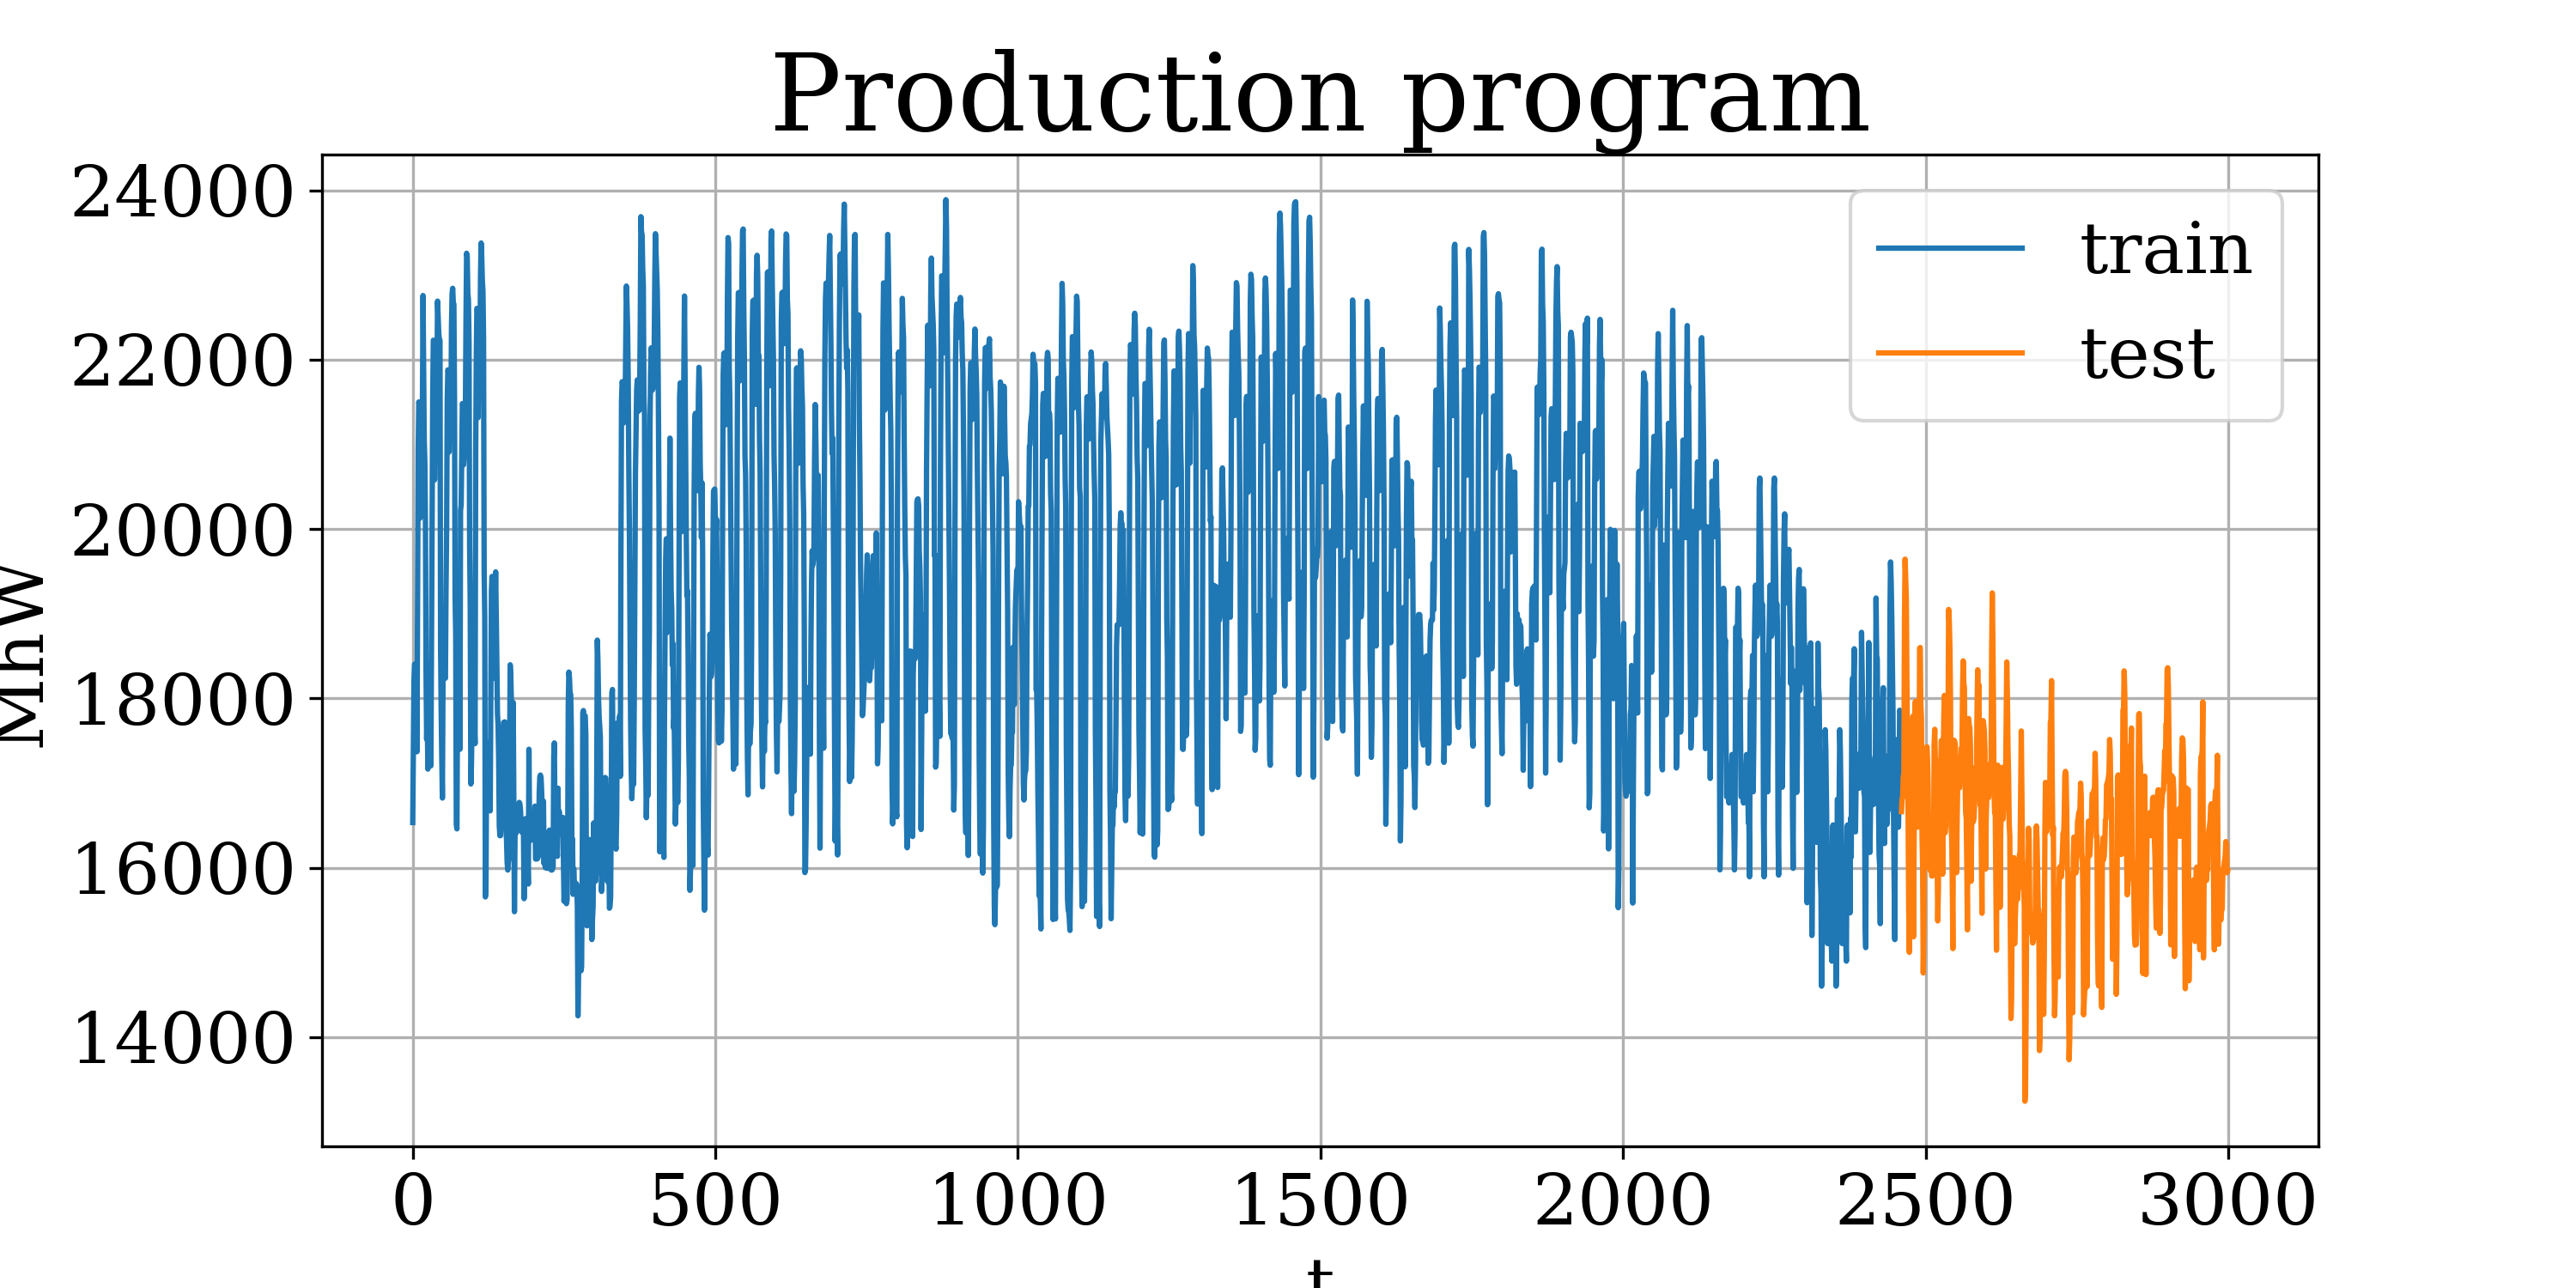
\includegraphics[width=0.43\textwidth, keepaspectratio]{../../figs/Electricity_Production}
		 	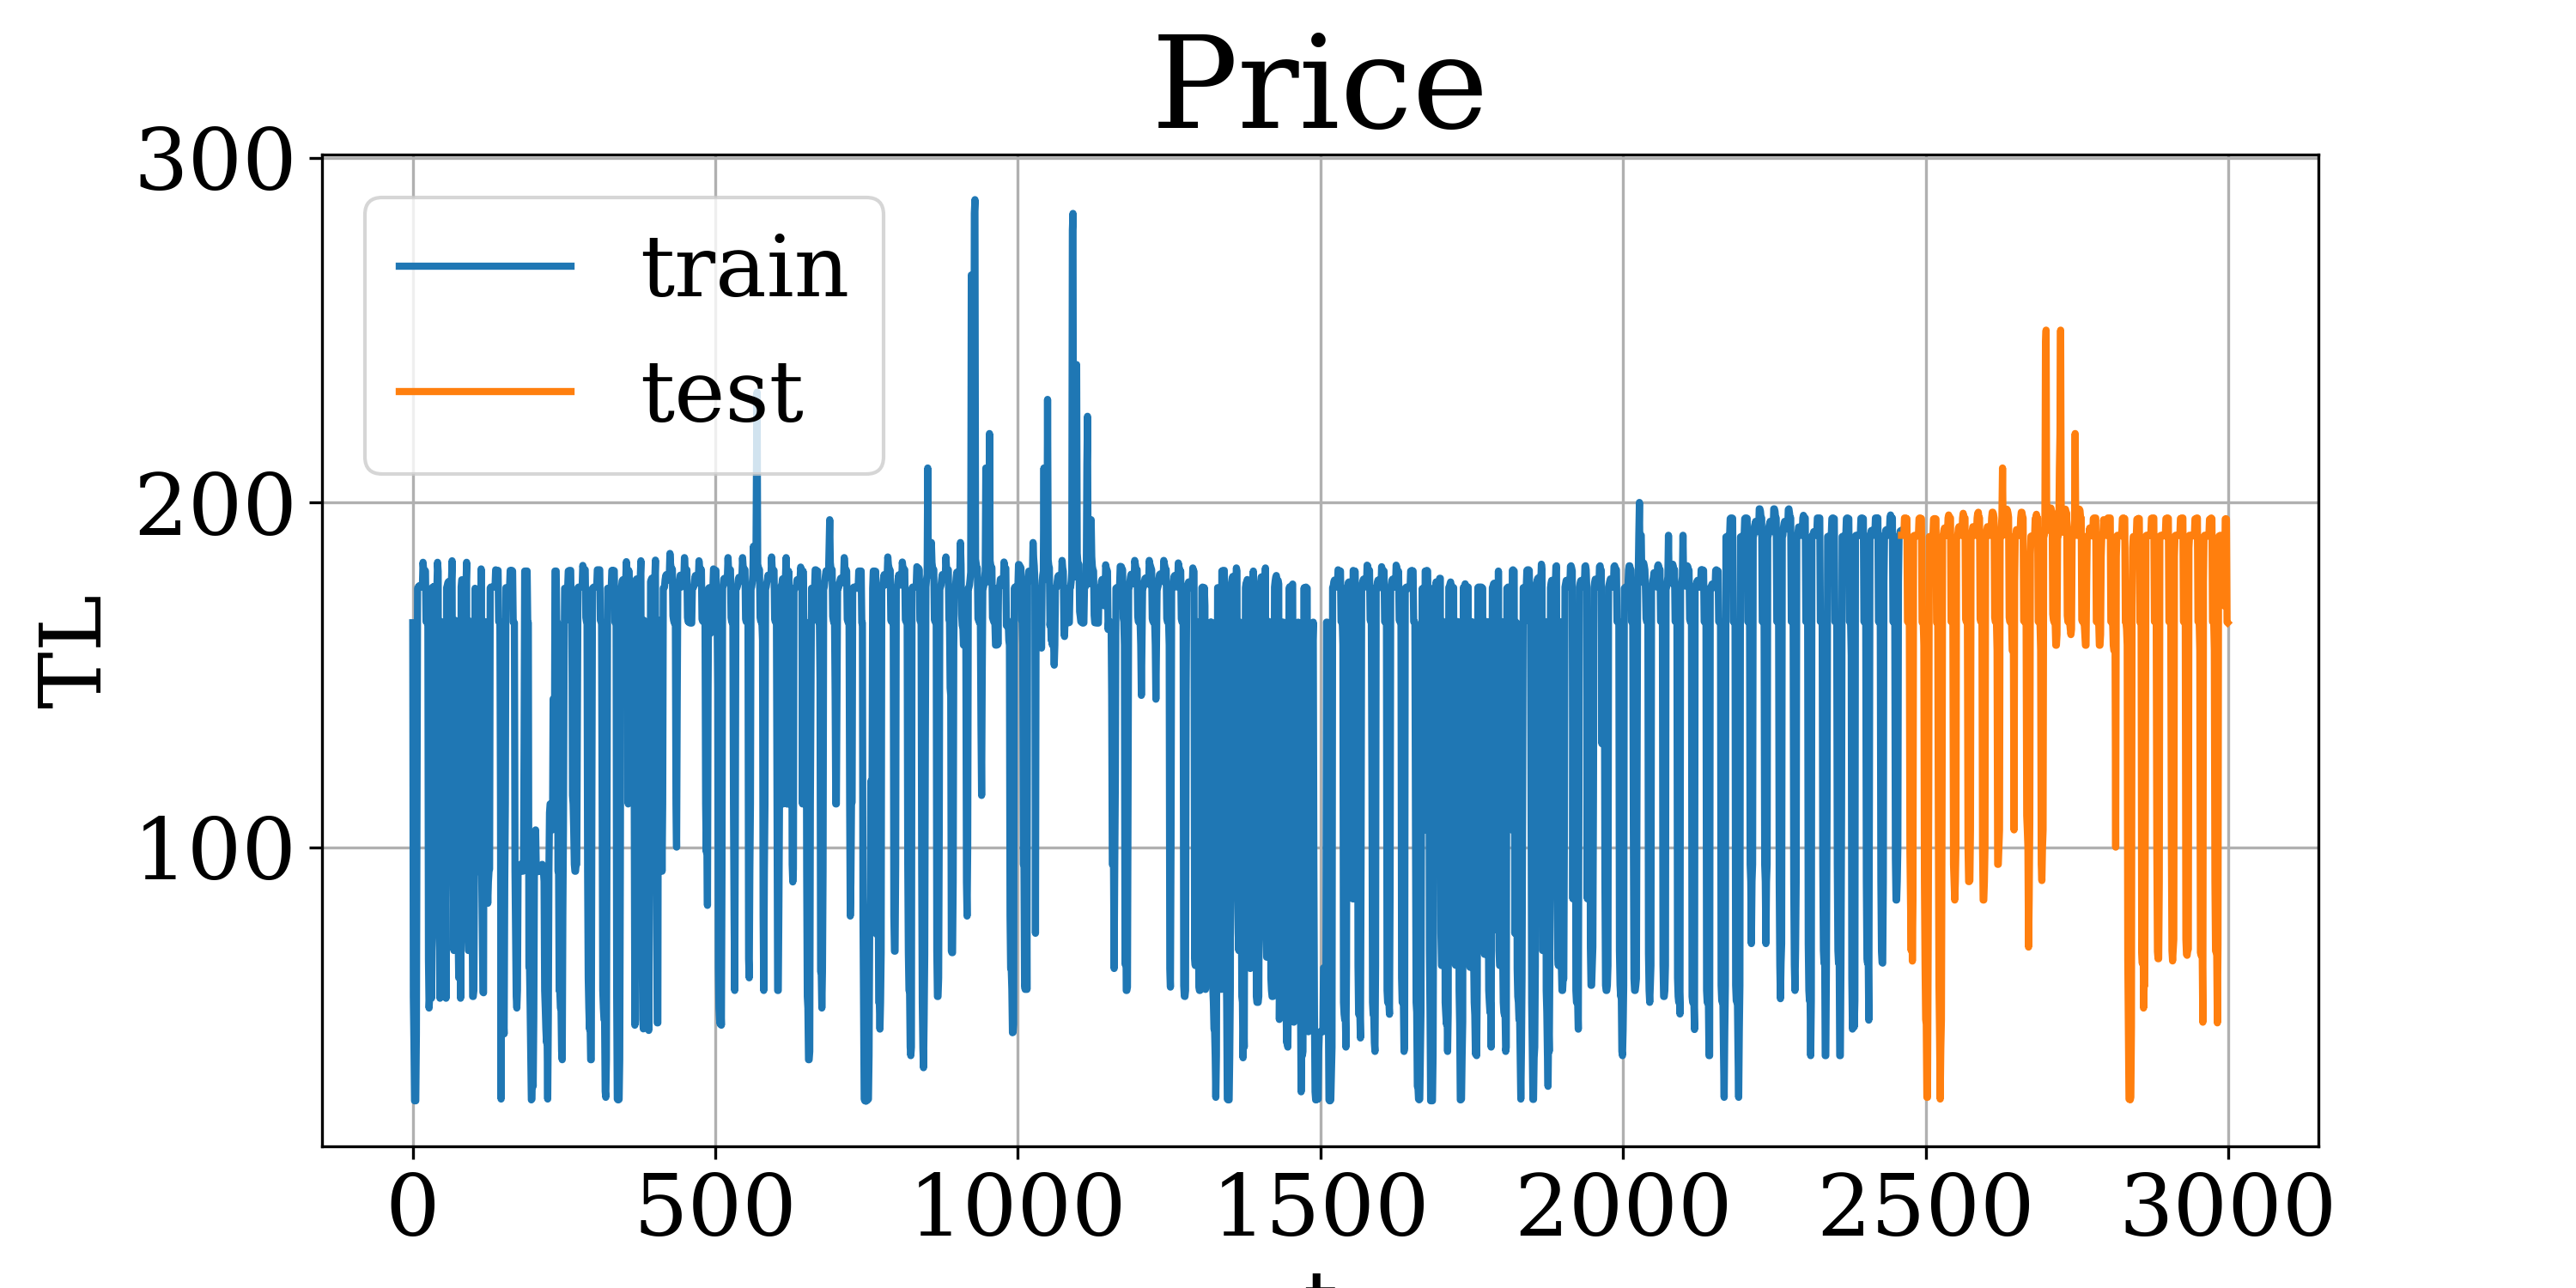
\includegraphics[width=0.43\textwidth, keepaspectratio]{../../figs/Electricity_Price}
		 	\caption{Потребление электричества и его цены за единицу мощности}\label{fig:electr_data}
		 \end{figure}
		
	\end{frame}
	
	\begin{frame}{Метрики декомпозиции}
		
		\begin{Def}
			\emph{Абсолютной ошибкой ганкелизации} матрицы M назовём 
			
			\[
			\text{AHE} = \lVert M - \text{Hankel}(M) \rVert_2
			\] 
		\end{Def}
		
		\begin{Def}		
			
			\emph{Относительной ошибкой ганкелизации} матрицы M назовём 
			
			\[
			\text{RHE} = \frac{\text{AHE}}{\lVert M \rVert_2} 
			\] 		
			
		\end{Def}
		
		AHE имеет смысл суммарного стандартного отклонения антидиагоналей матрицы. RHE её более интерпретируемая модификация. 
		
		Данные метрики будут применяться к матрицам группировки факторов $ C_i $.
	
	\end{frame}
	
	\begin{frame}{Зависимость качества прогноза от CP-ранга}
		
		\begin{center}
			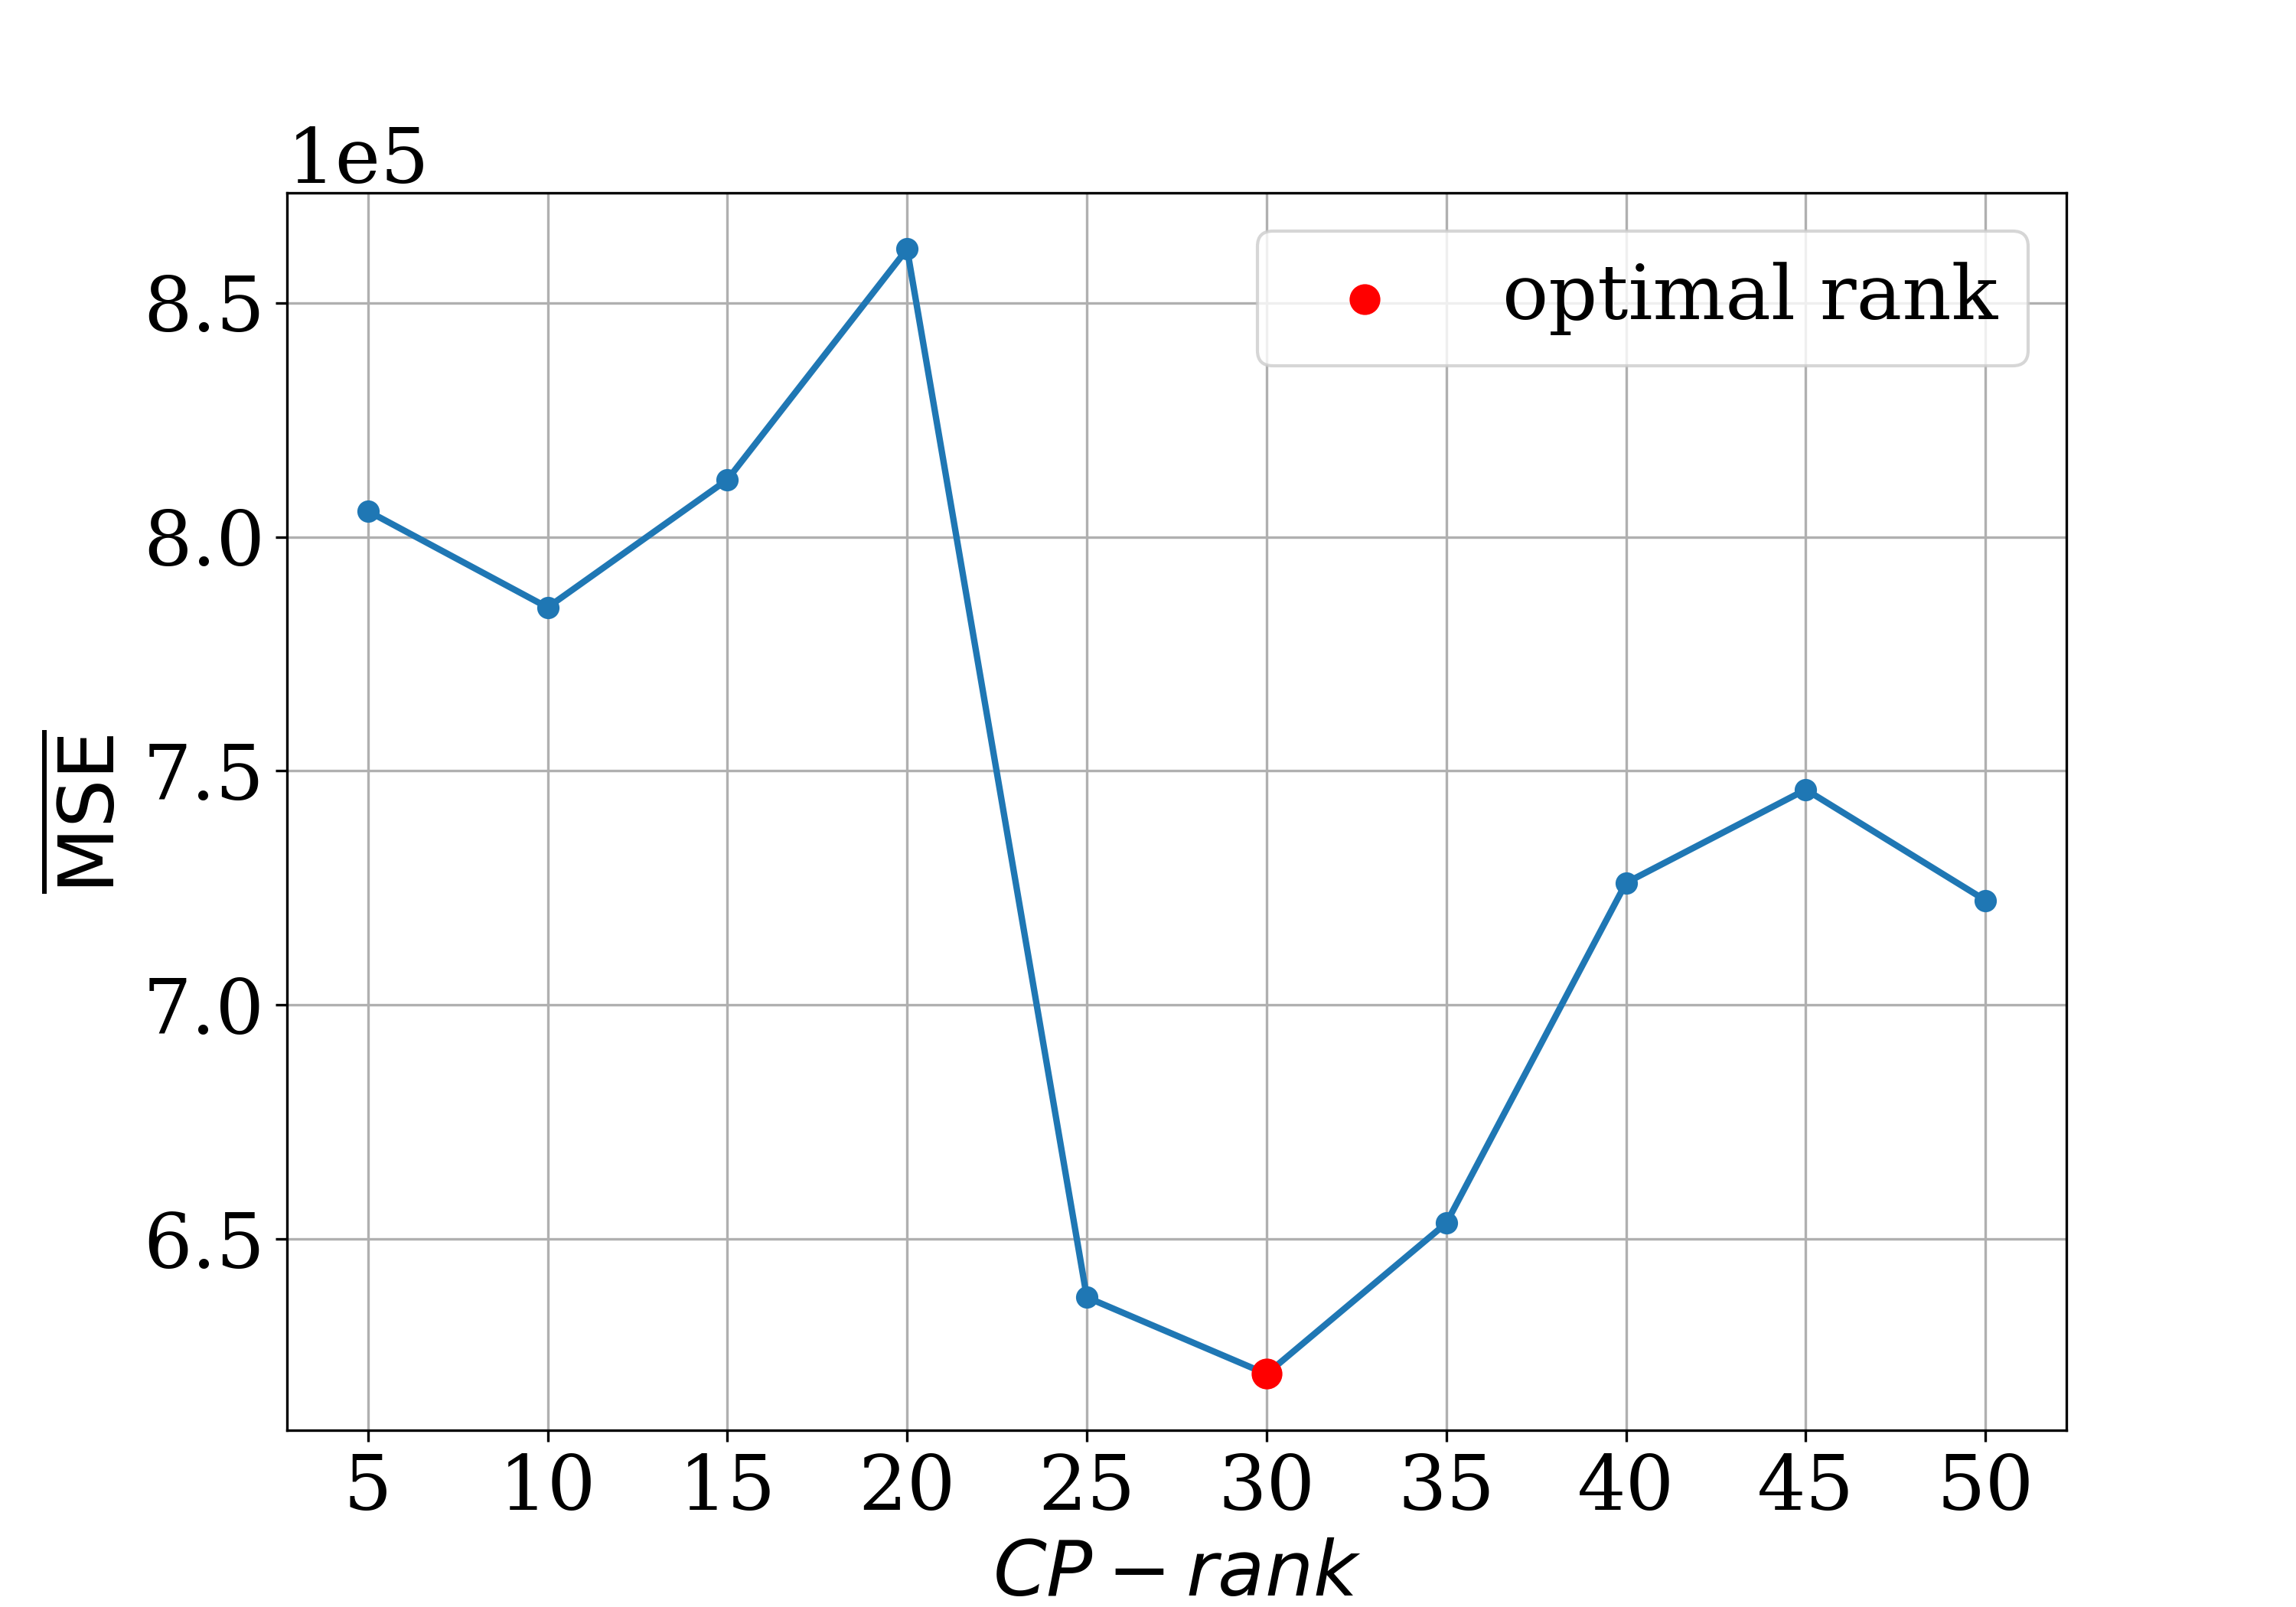
\includegraphics[width=0.33\textwidth, keepaspectratio]{../../experiments/electricity/tssa/figs/prediction/MSE_rank.png}
			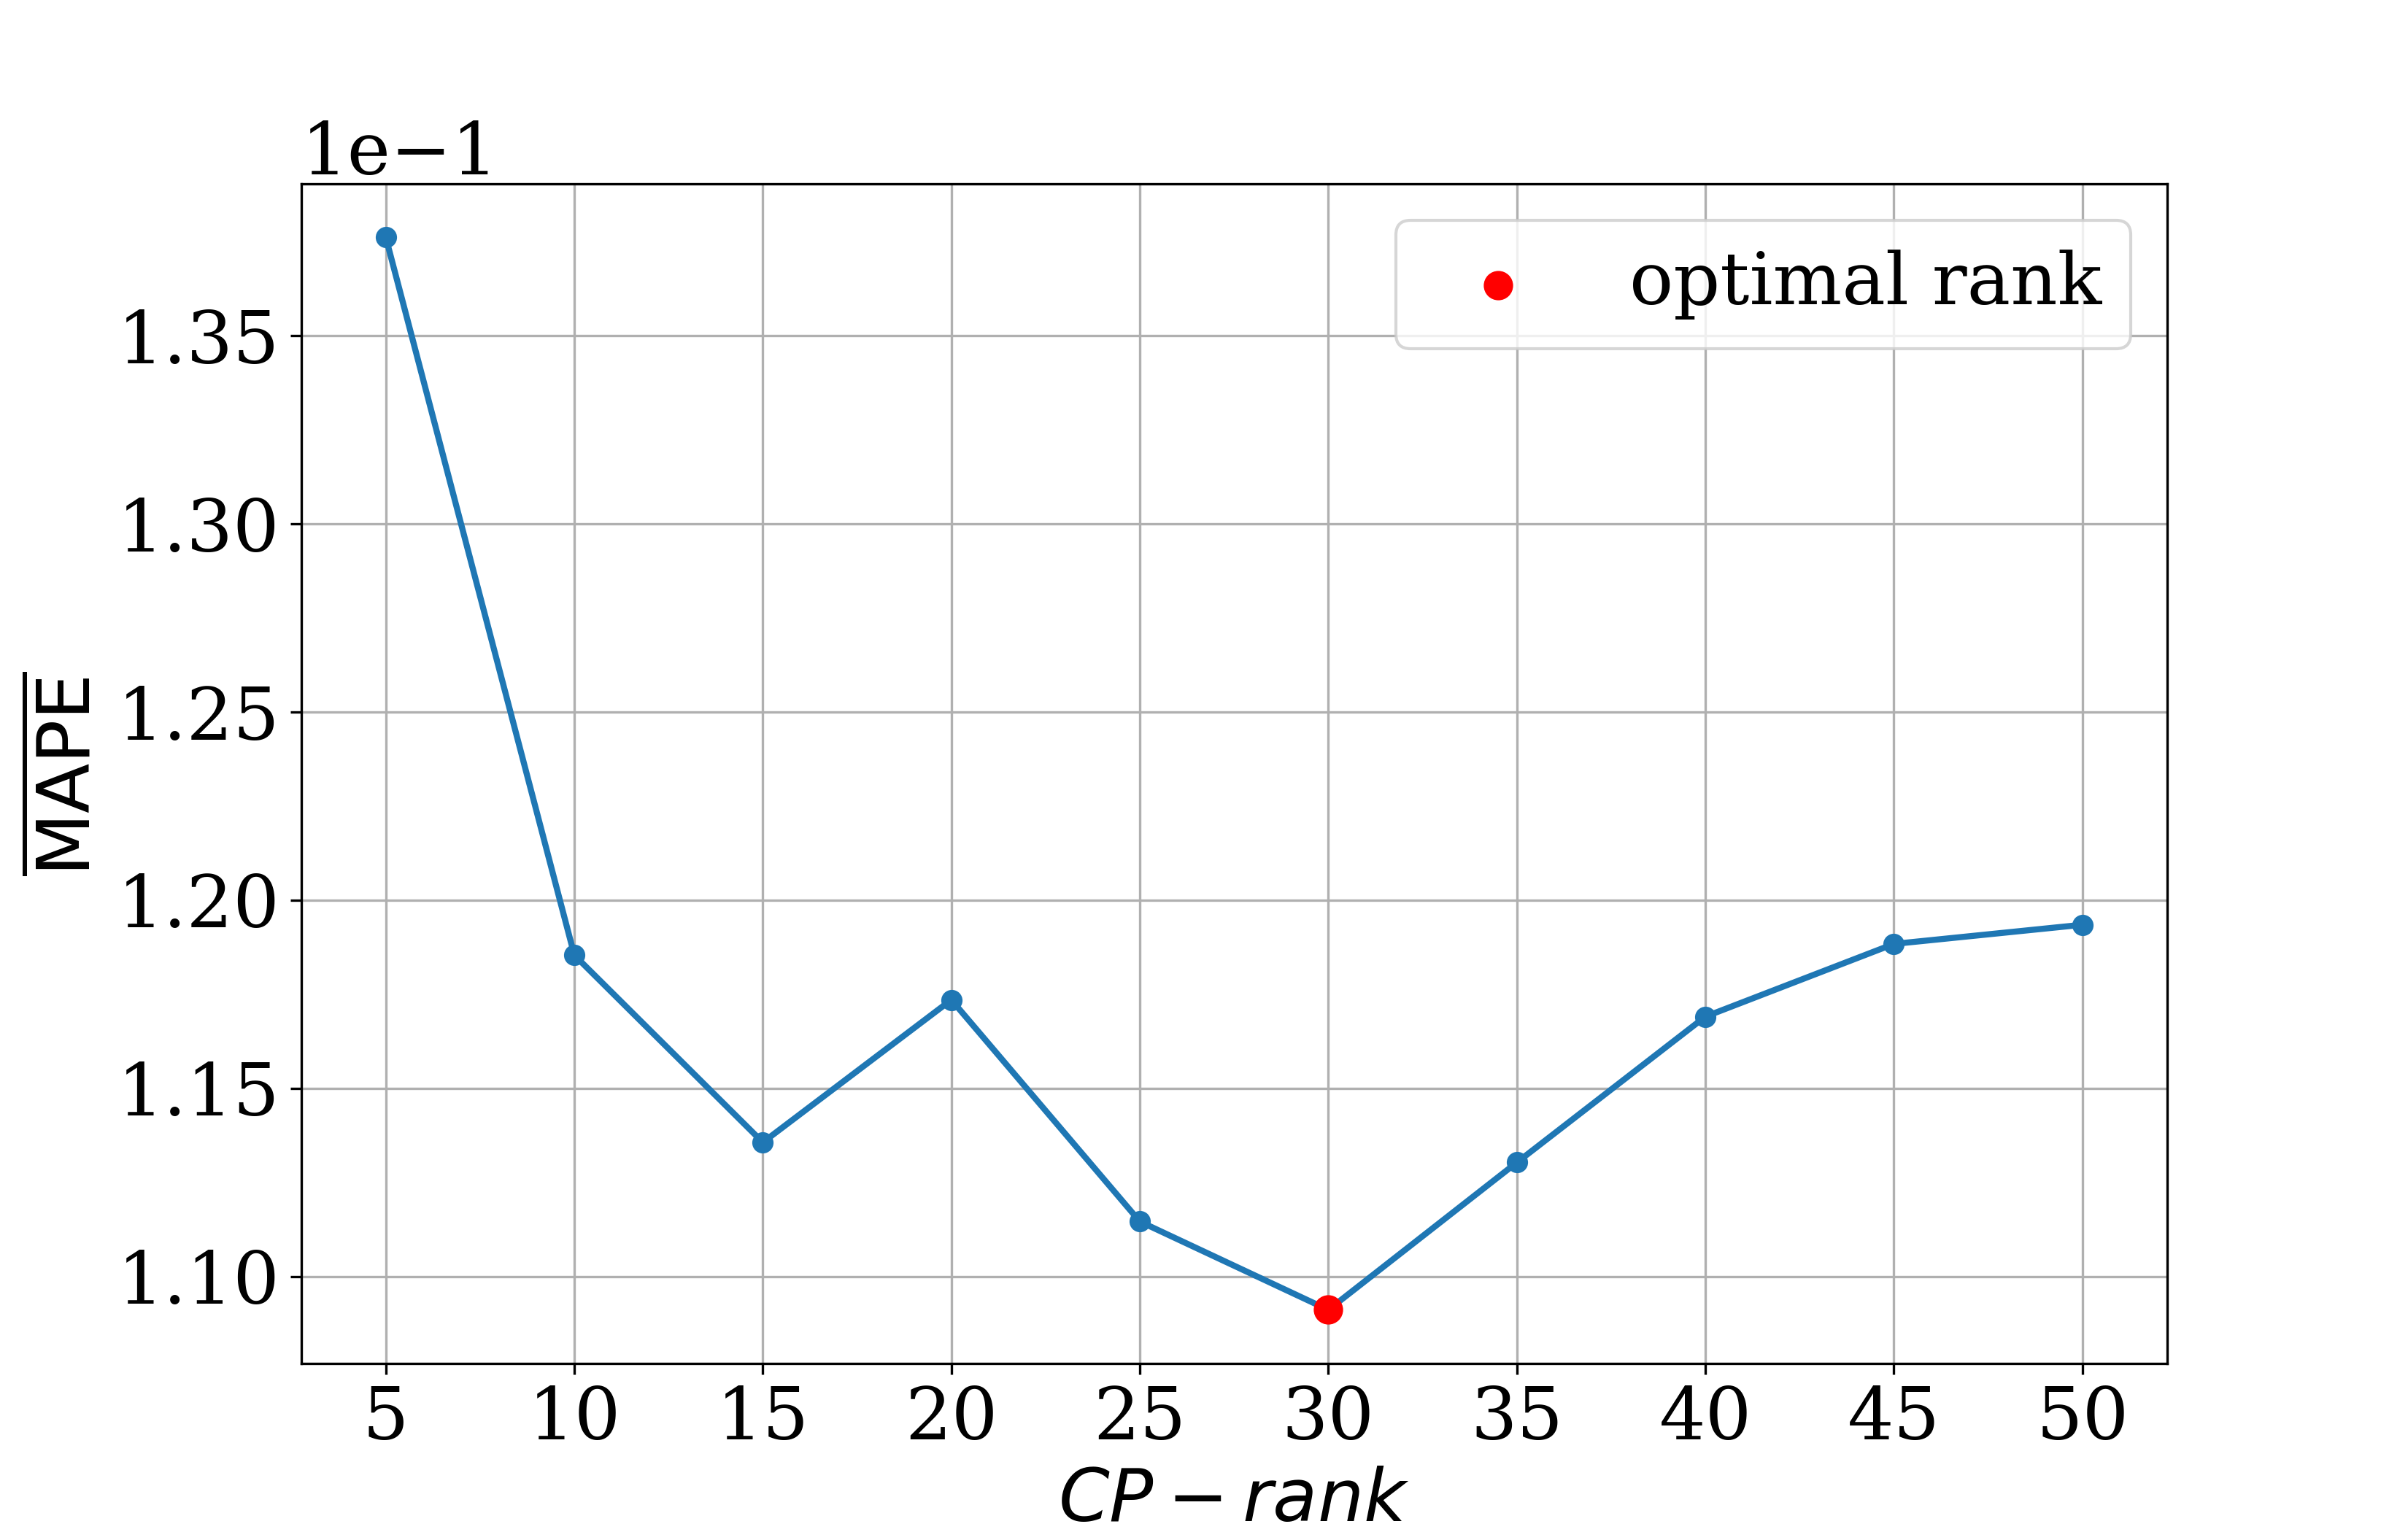
\includegraphics[width=0.33\textwidth, keepaspectratio]{../../experiments/electricity/tssa/figs/prediction/MAPE_rank.png} \\
			{\small Данные электроэнергии.} \\
			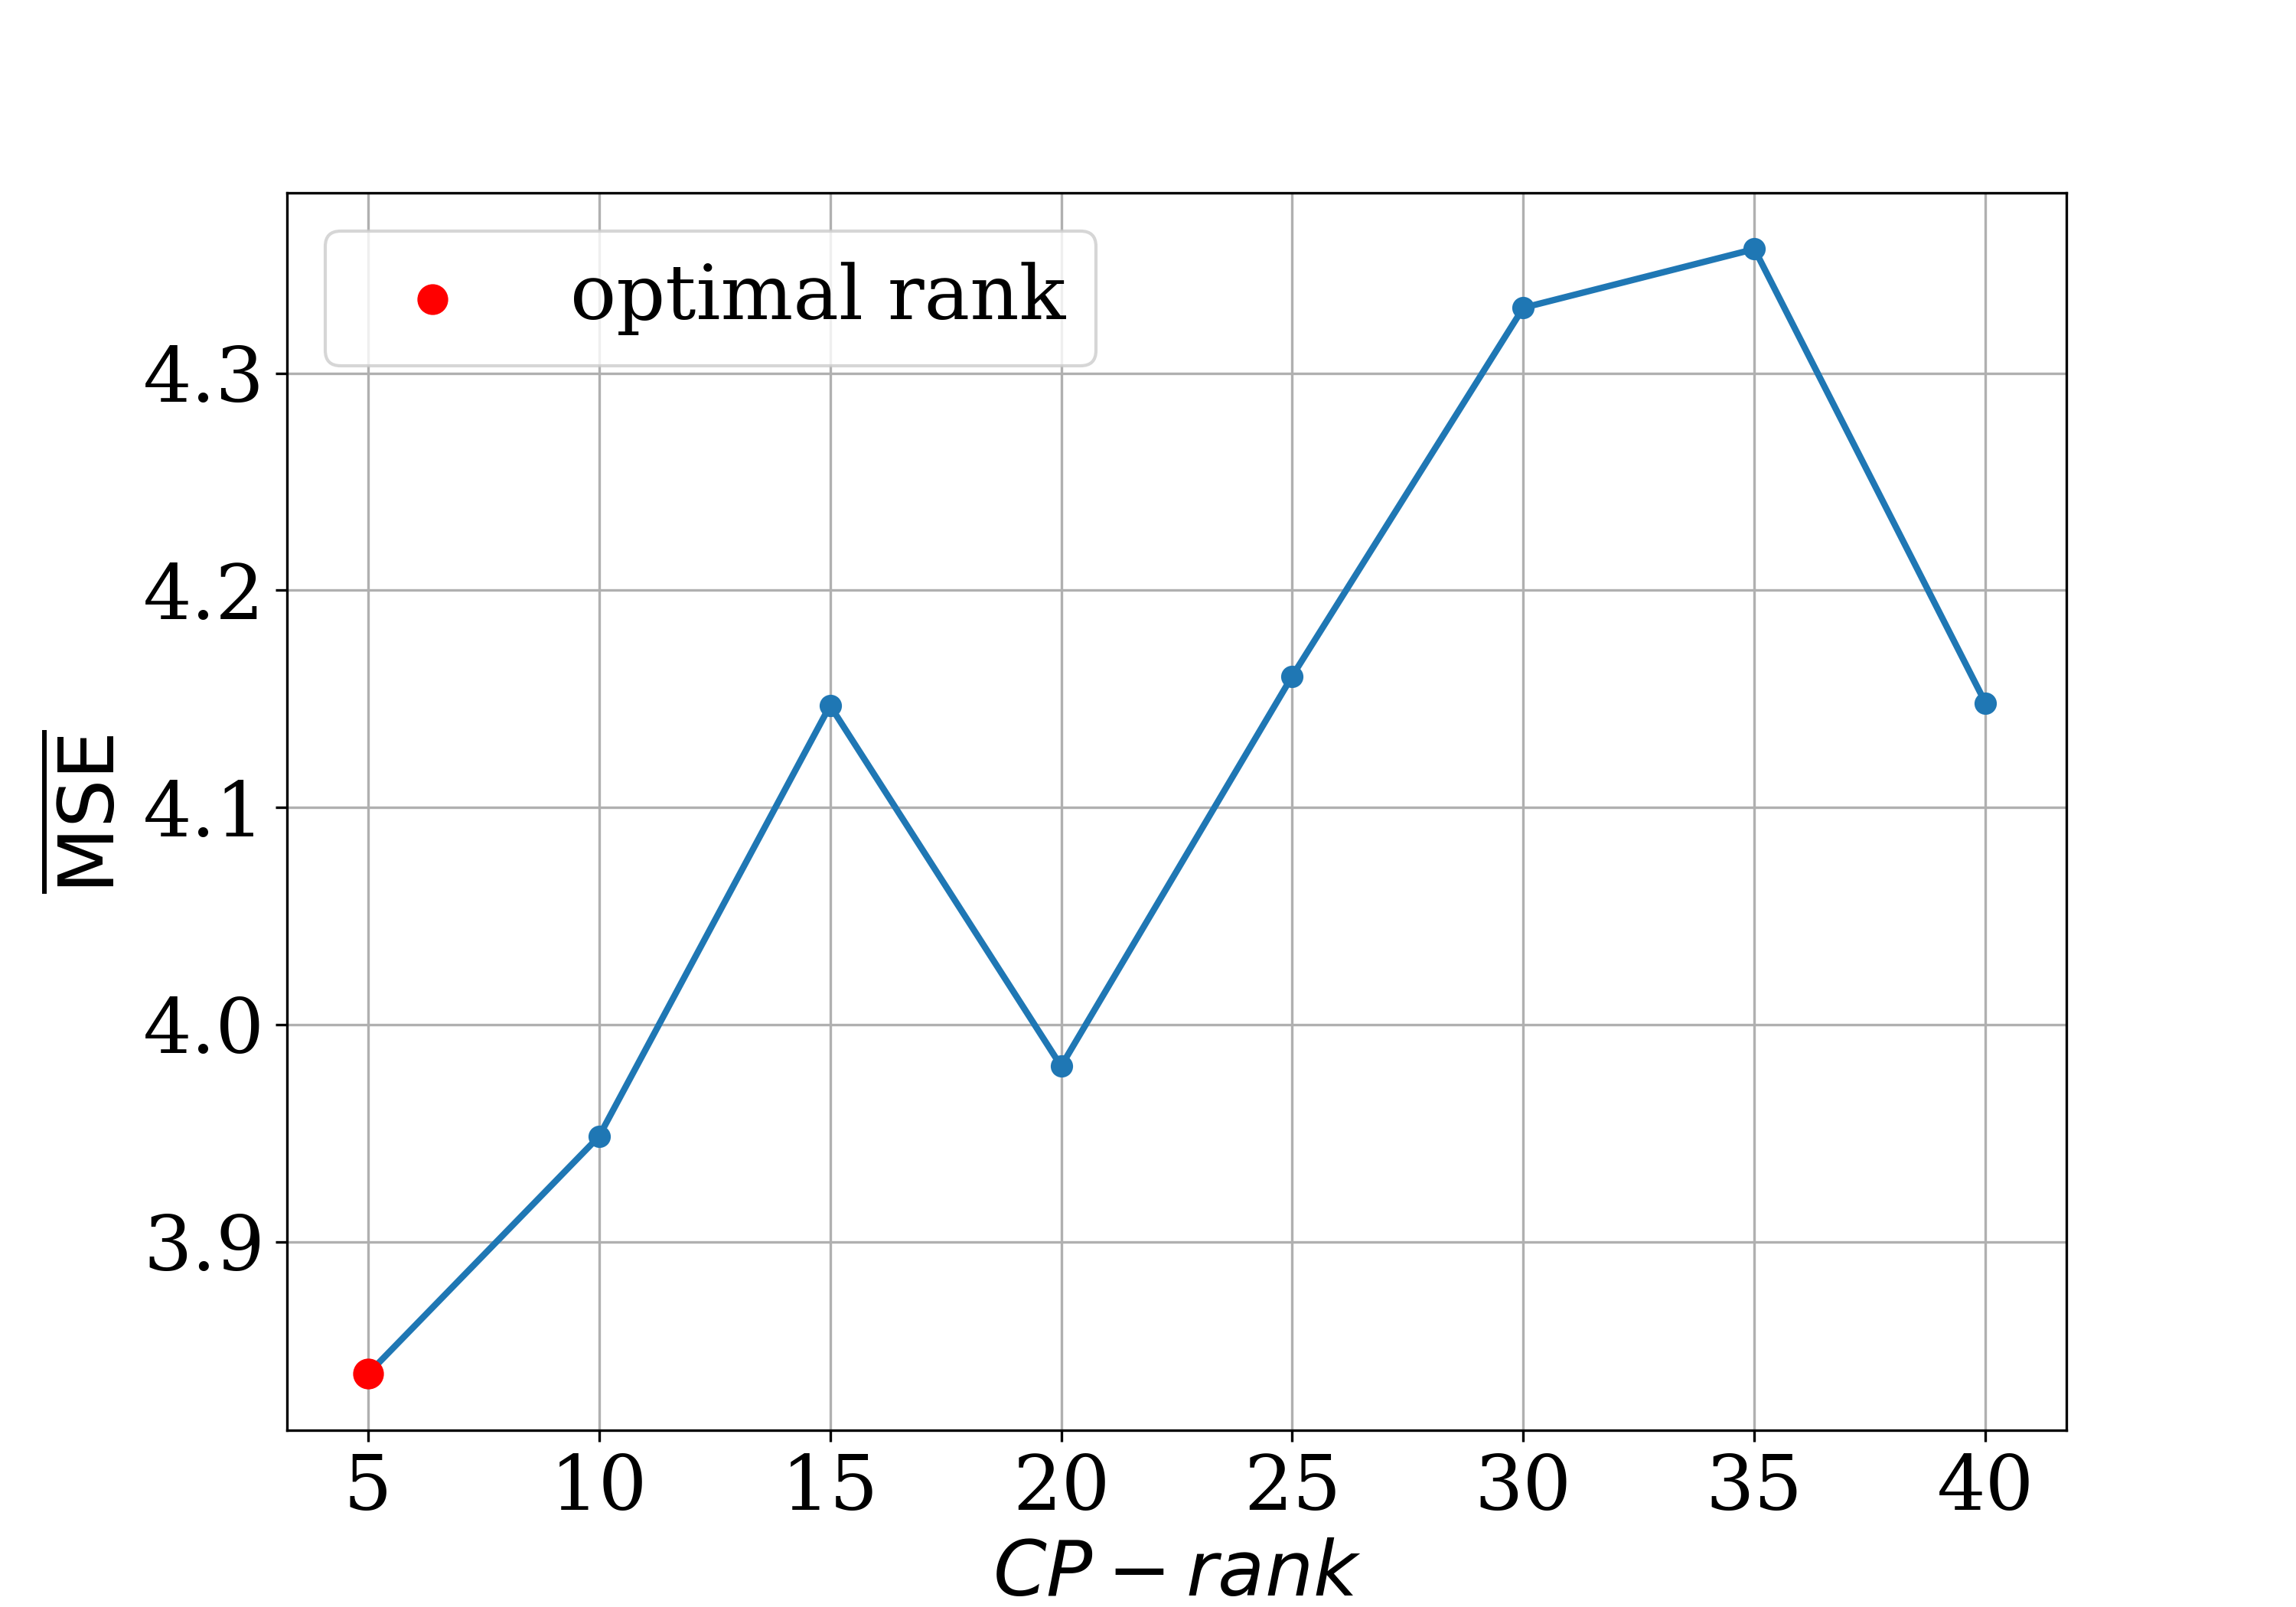
\includegraphics[width=0.33\textwidth, keepaspectratio]{../../experiments/motion_1/tssa/figs/prediction/MSE_rank.png}
			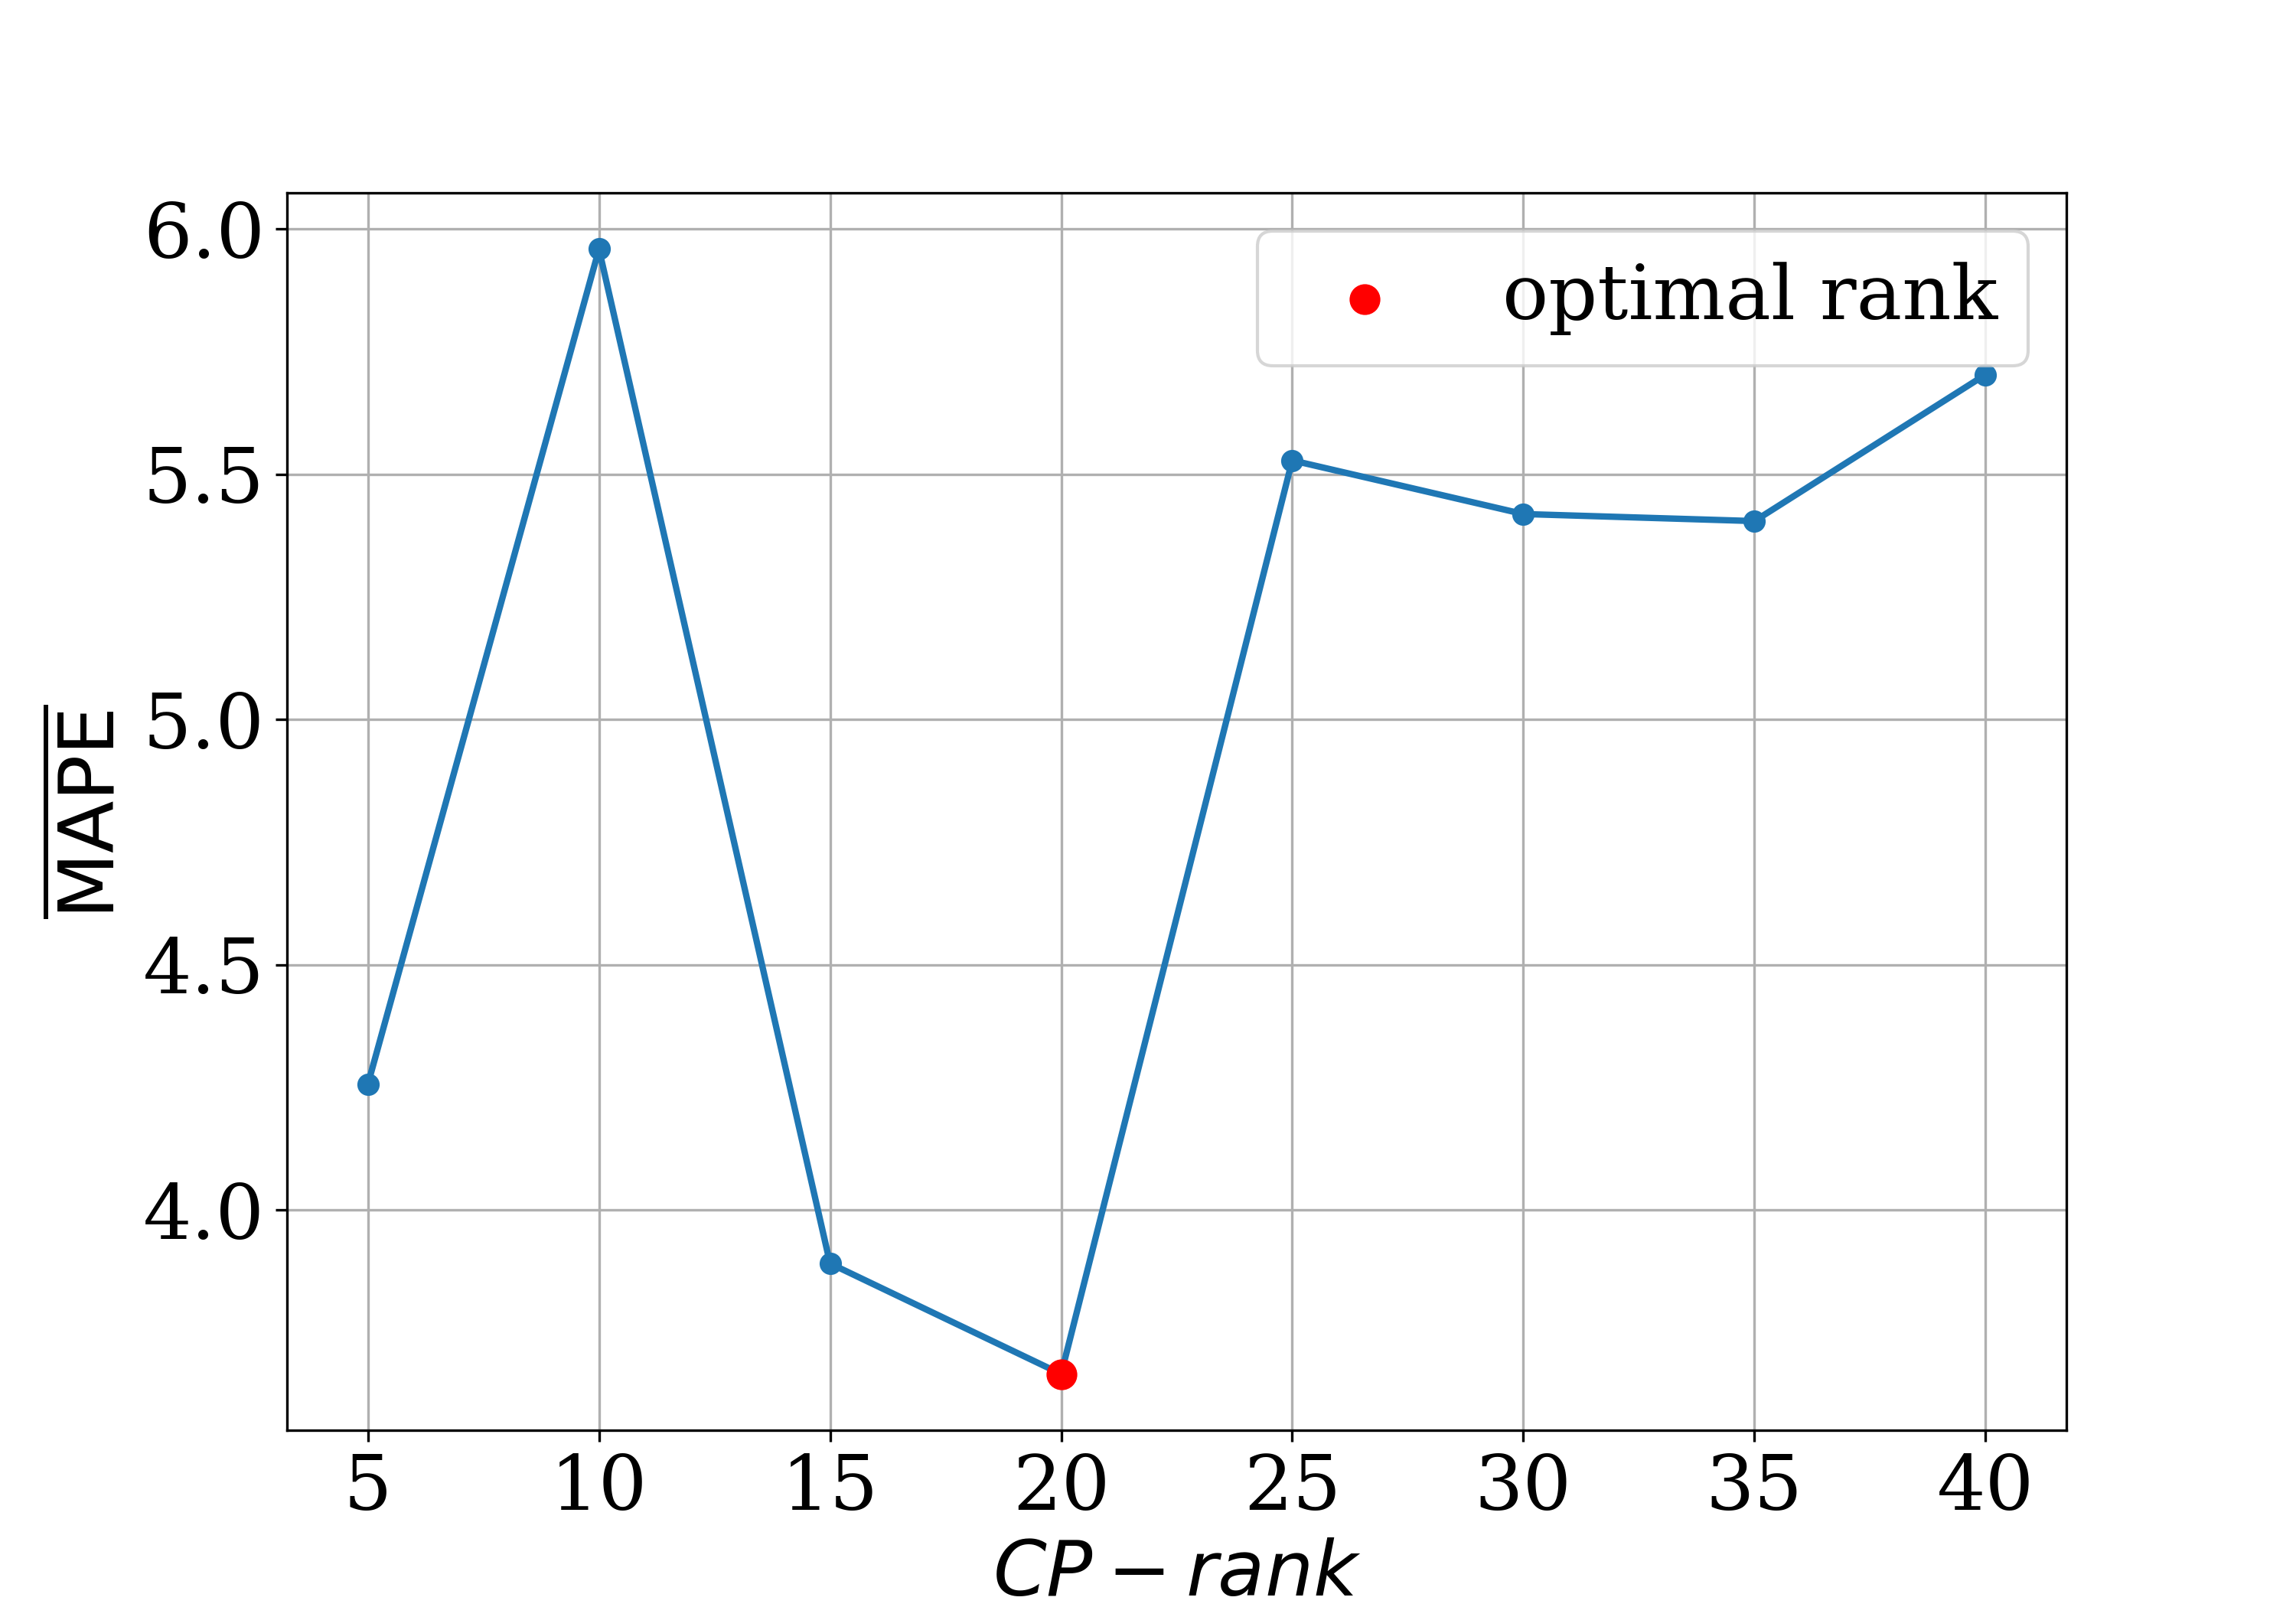
\includegraphics[width=0.33\textwidth, keepaspectratio]{../../experiments/motion_1/tssa/figs/prediction/MAPE_rank.png} \\
			{\small Данные акселерометрии.} \\
		\end{center}
		
		Отдельно выделен оптимальный ранг. Наблюдается эффект переобучения при возрастании ранга.
		
	\end{frame}
	
	\begin{frame}{Визуализация прогноза методом tSSA}
		
		\begin{center}
			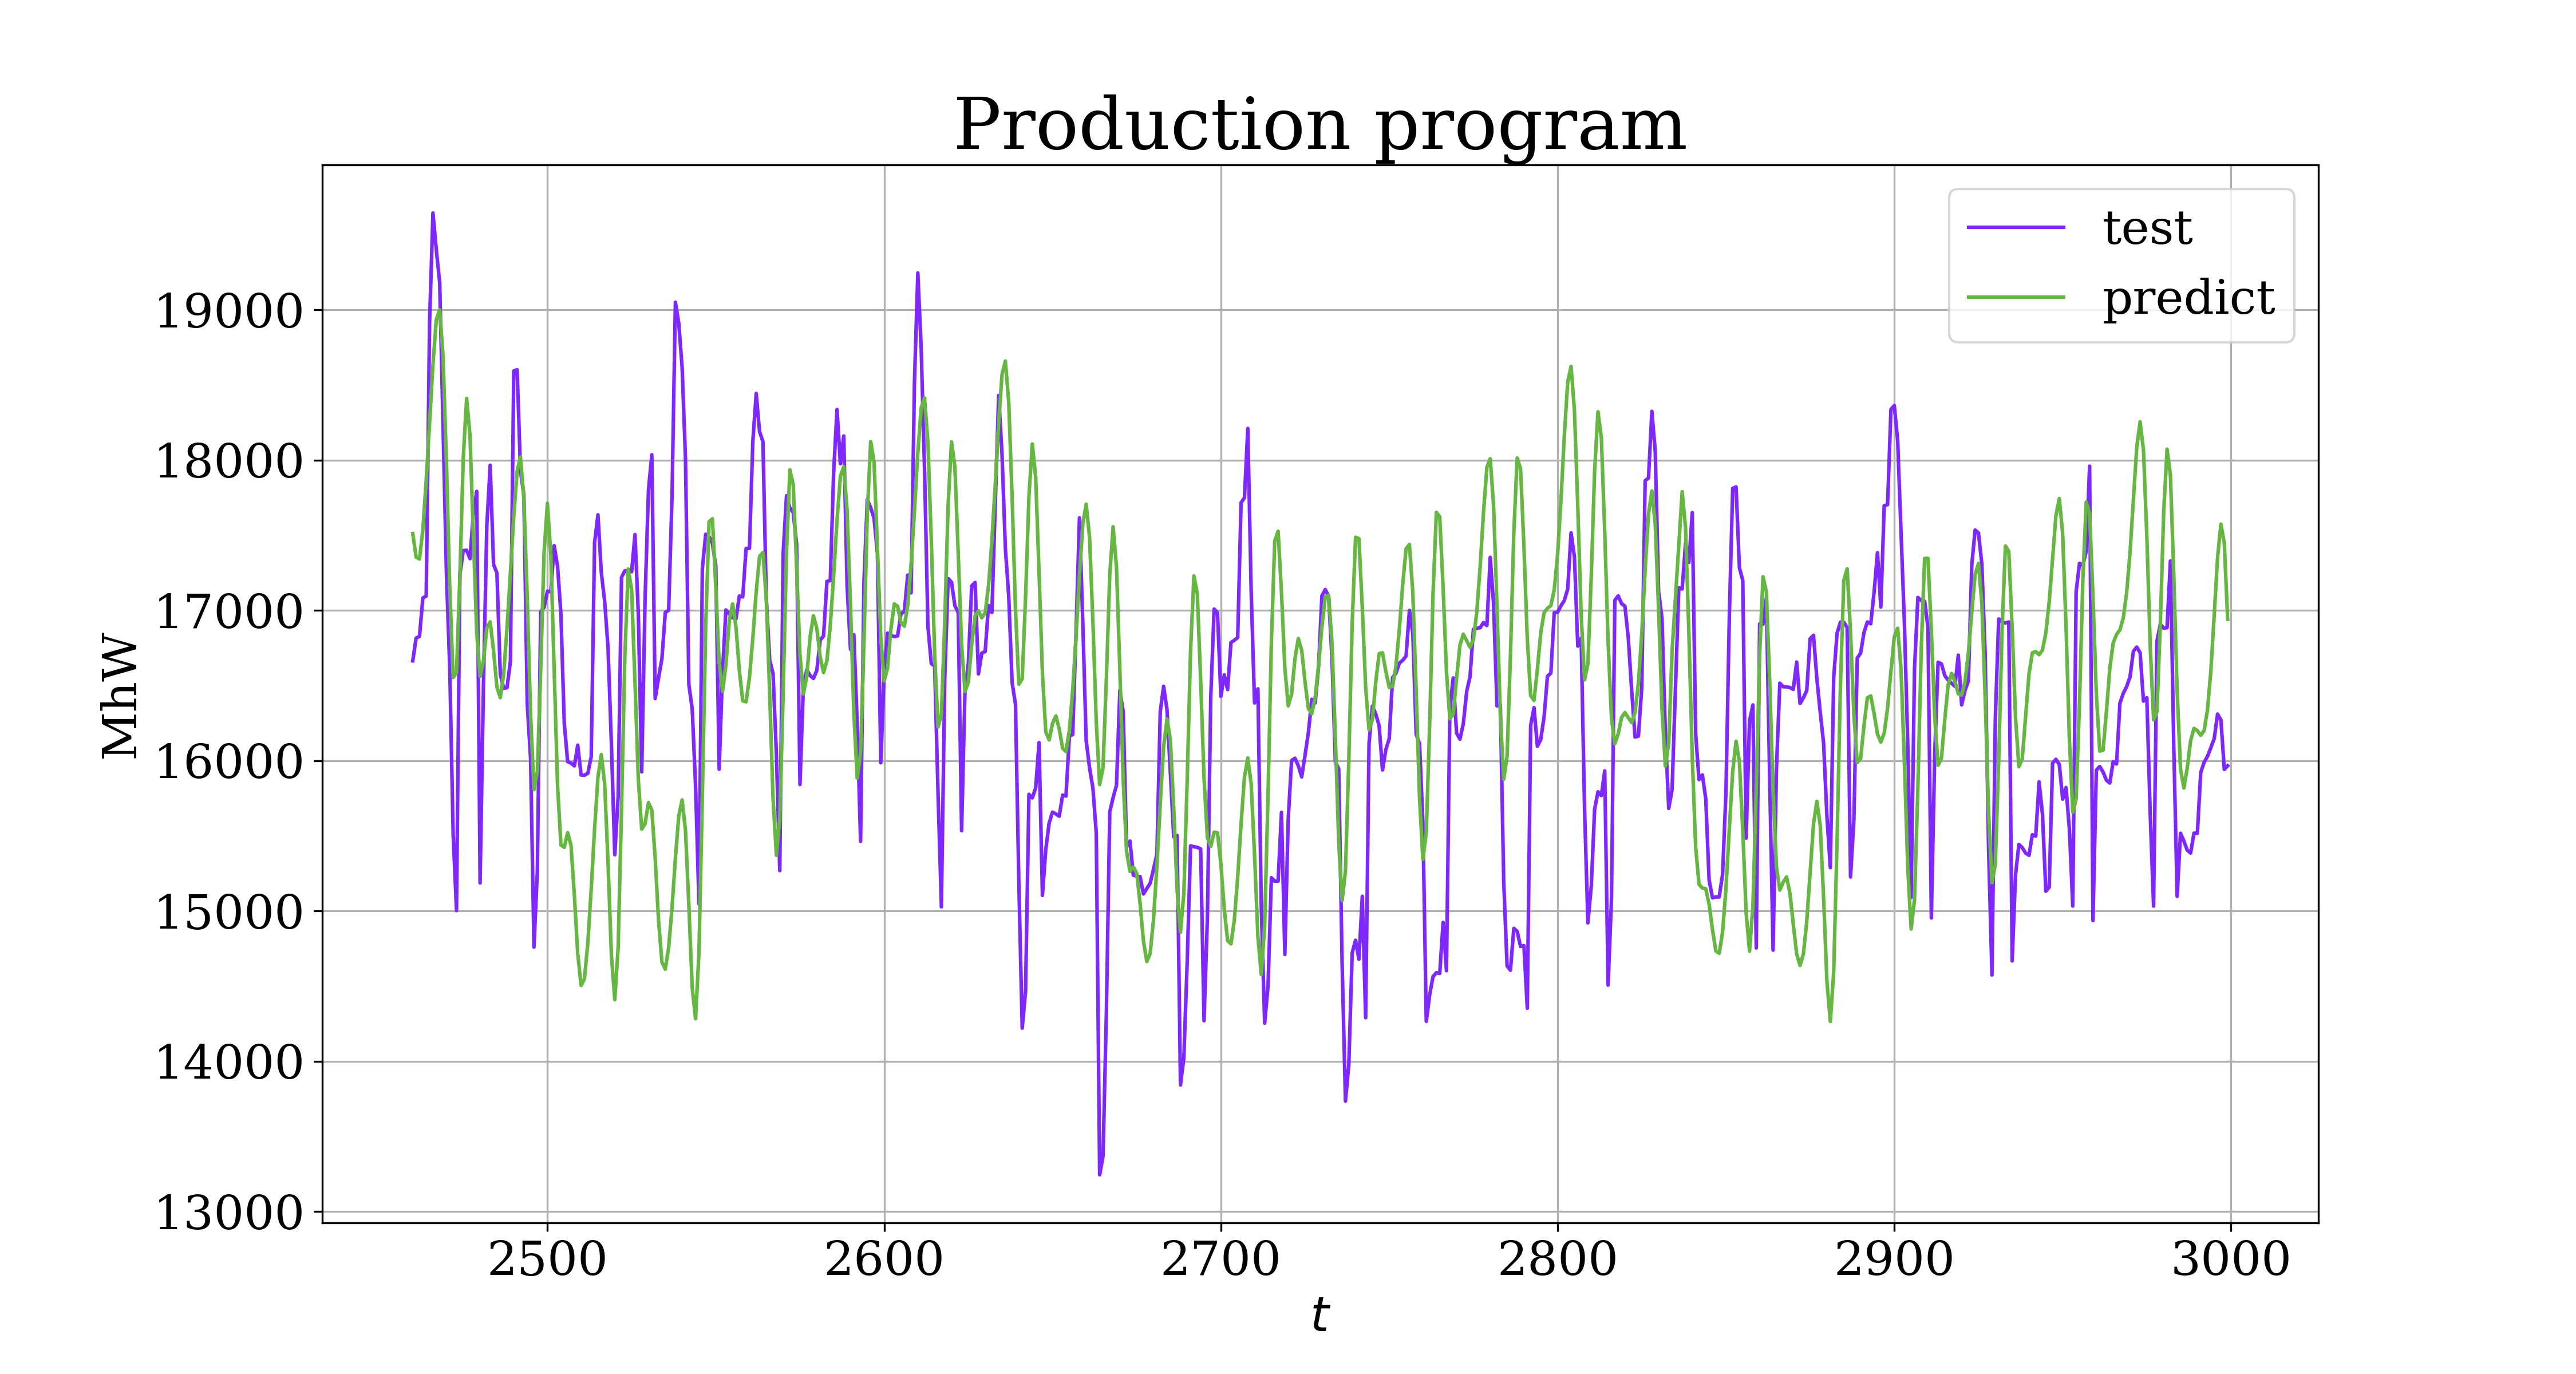
\includegraphics[width=0.43\textwidth, keepaspectratio]{../../experiments/electricity/tssa/figs/prediction/cpd_rank_30/Production_program.png}
			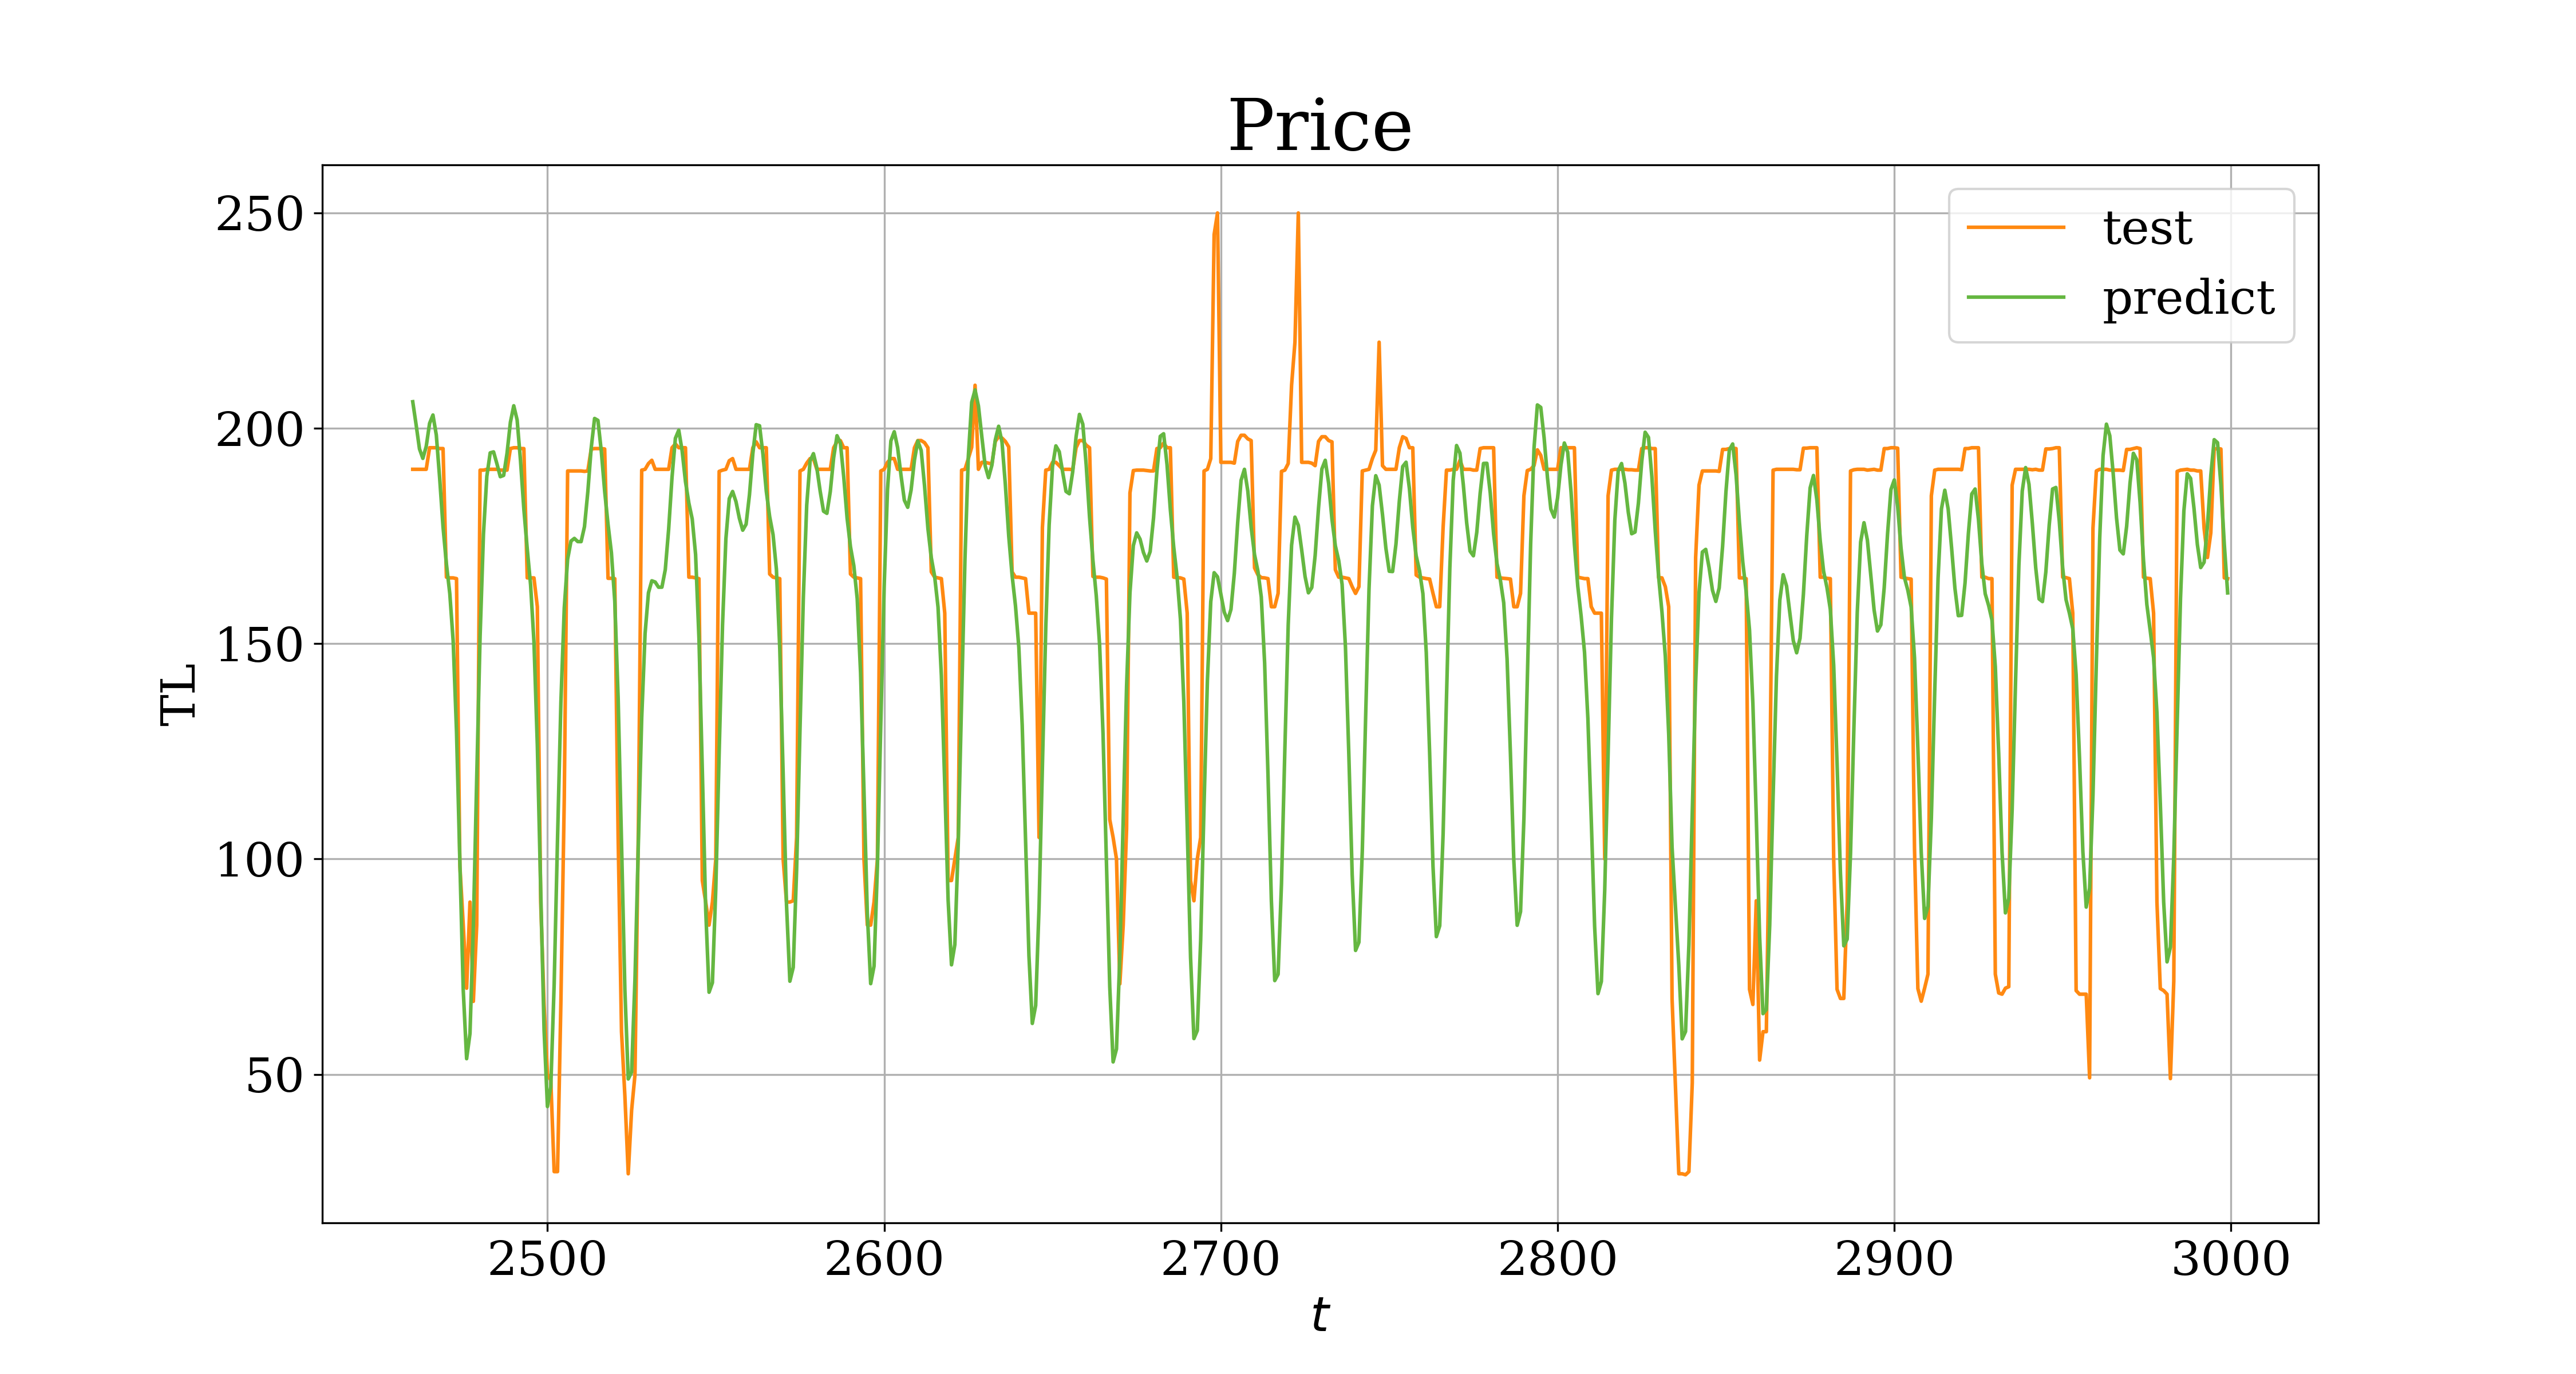
\includegraphics[width=0.43\textwidth, keepaspectratio]{../../experiments/electricity/tssa/figs/prediction/cpd_rank_30/Price.png} \\
			{\small Данные электроэнергии. CPD-ранг $ = 30 $.} \\ \vspace{0.2cm}
			
			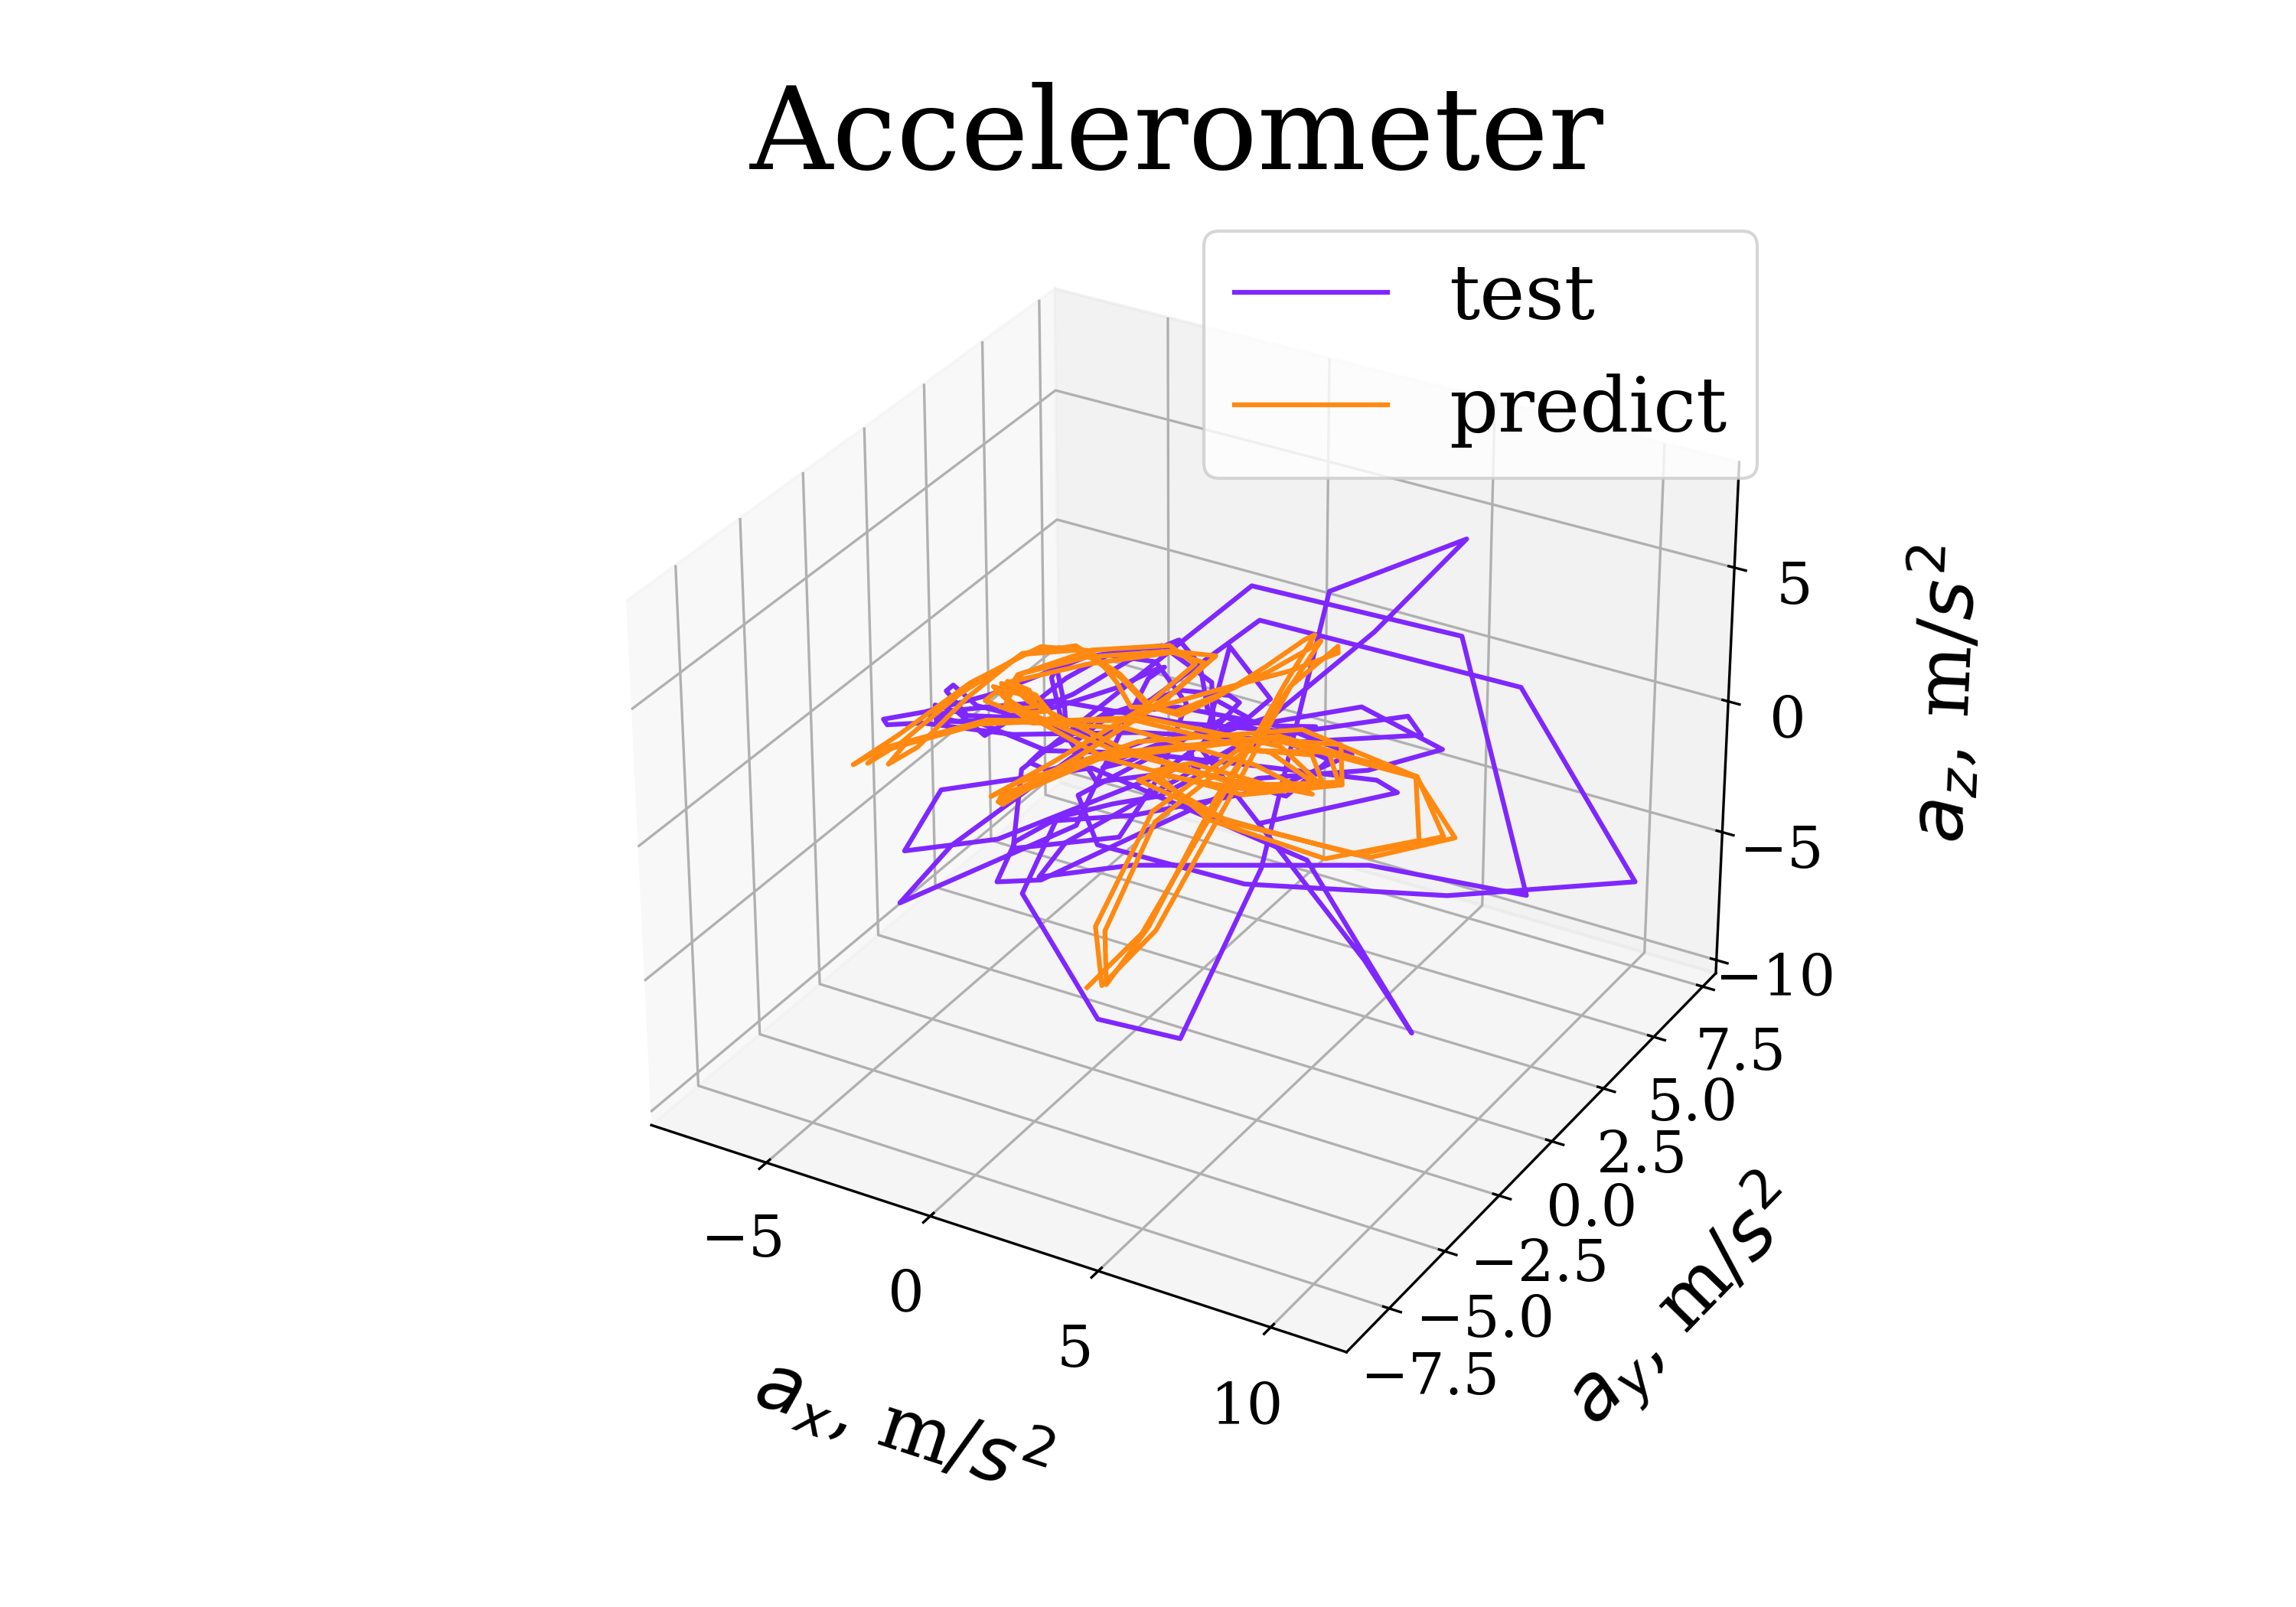
\includegraphics[width=0.43\textwidth, keepaspectratio]{../../experiments/motion_1/tssa/figs/prediction/cpd_rank_20/acceler.png}
			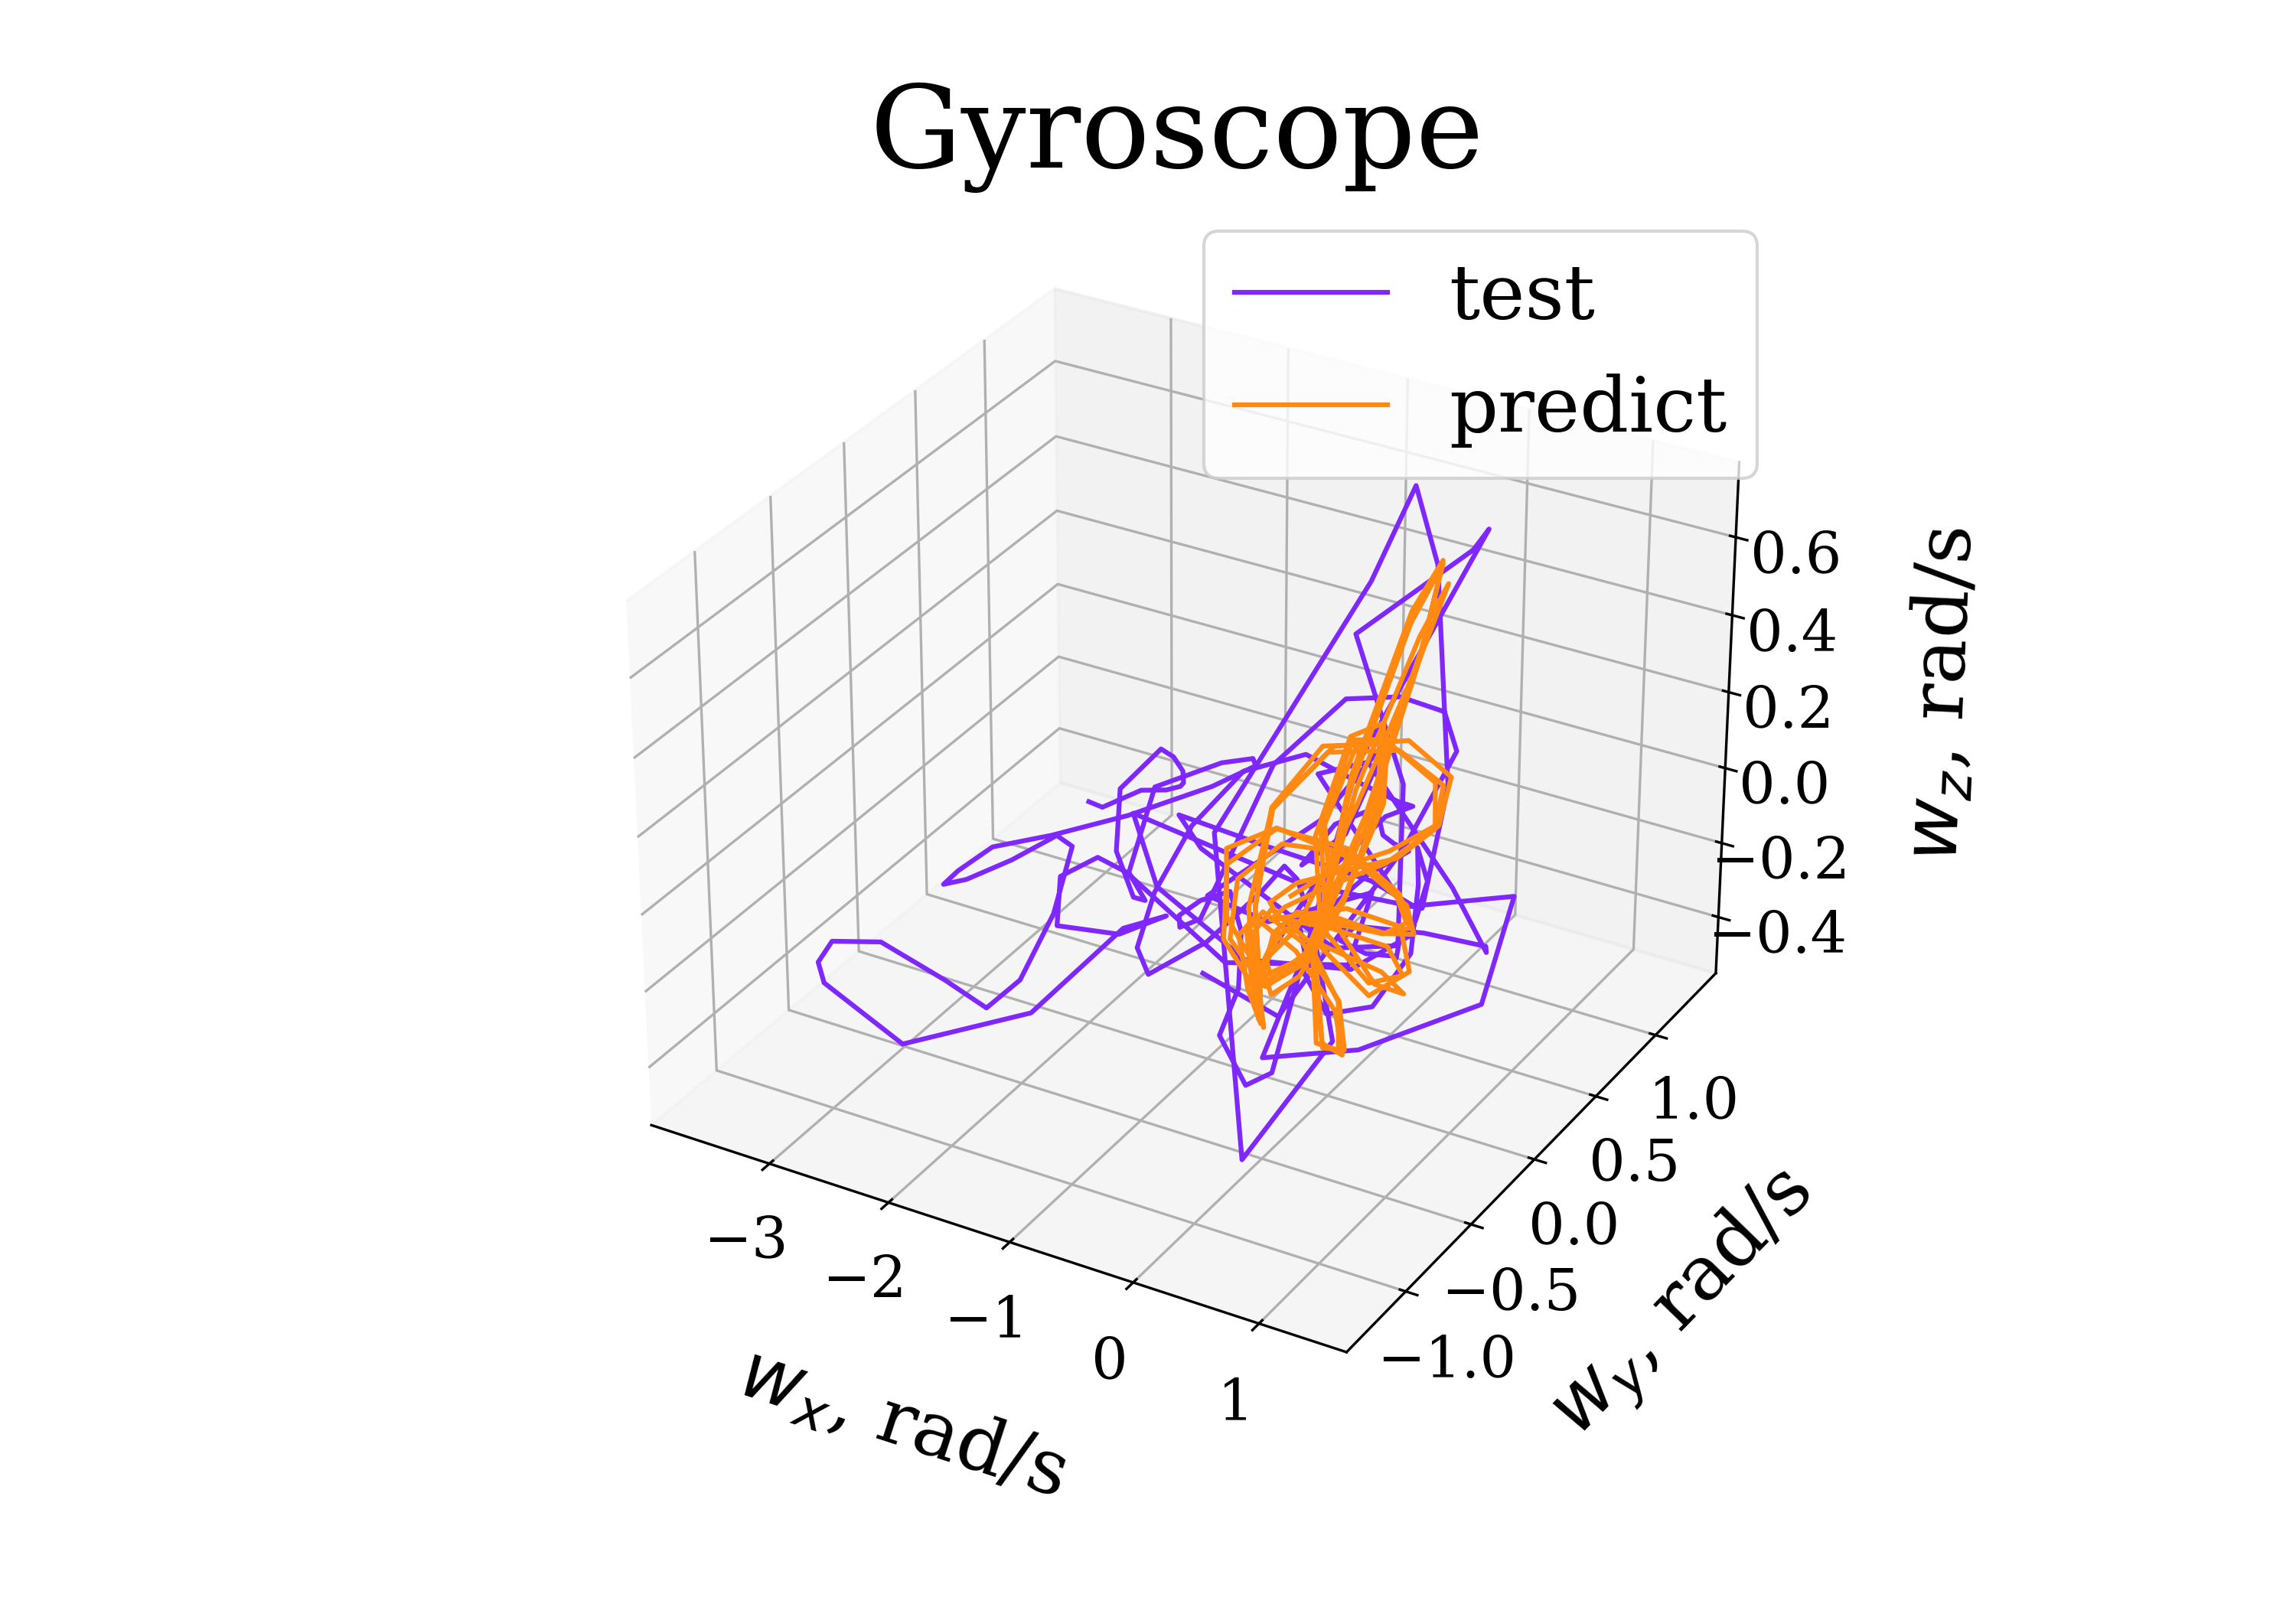
\includegraphics[width=0.43\textwidth, keepaspectratio]{../../experiments/motion_1/tssa/figs/prediction/cpd_rank_20/gyro.png} \\
			{\small Данные акселерометрии. CPD-ранг $ = 20 $.} \\
		\end{center}
		
		Тензорный ранг влияет на порядок модели прогноза.
		
	\end{frame}
	
	\begin{frame}{Качество прогноза моделей}
		
		\begin{center}
			{\small Данные электроэнергии.} \\
			\scalebox{0.6}{
				\begin{tabular}{|c|c|c|c|c|}
					\hline
					& \textit{tSSA}  & \textit{mSSA} & \textit{VAR} & \textit{RNN} \\ \hline
					$ \overline{\text{MSE}}_{\text{Producution}} $, $10^6$ & 1.24           & 1.51          & 7.81         & 2.70         \\ \hline
					$ \overline{\text{MSE}}_{\text{Price}} $, $10^3$      & 0.88           & 1.03          & 4.85         & 30.0         \\ \hline
					$ \overline{\text{MSE}} $, $10^6$             & \textbf{0.62}  & 0.75          & 3.91         & 135.00       \\ \hline
					$ \overline{\text{MAPE}}_{\text{Producution}} $        & 0.054          & 0.060         & 0.137        & 0.999        \\ \hline
					$ \overline{\text{MAPE}}_{\text{Price}} $             & 0.164          & 0.170         & 0.360        & 1.004        \\ \hline
					$ \overline{\text{MAPE}} $                    & \textbf{0.109} & 0.115         & 0.249        & 1.002        \\ \hline
				\end{tabular}
			}
		\end{center}
		
		\begin{center}
			{\small Данные акселерометрии.} \\
			\scalebox{0.6}{
				\begin{tabular}{|c|c|c|c|c|}
					\hline
					& \textit{tSSA}                & \textit{mSSA} & \textit{VAR} & \textit{RNN} \\ \hline
					$ \overline{\text{MSE}}_{\text{Accel}} $  & 7.351          & 6.980 & 8.108  & 6.604          \\ \hline
					$ \overline{\text{MSE}}_{\text{Gyro}} $   & 0.610          & 0.636 & 0.631  & 0.639          \\ \hline
					$ \overline{\text{MSE}} $         & 3.981          & 3.808 & 4.370  & \textbf{3.622} \\ \hline
					$ \overline{\text{MAPE}}_{\text{Accel}} $ & 3.558          & 3.516 & 3.370  & 1.747          \\ \hline
					$ \overline{\text{MAPE}}_{\text{Gyro}} $  & 3.773          & 3.943 & 10.427 & 5.641          \\ \hline
					$ \overline{\text{MAPE}} $        & \textbf{3.666} & 3.730 & 6.899  & 3.694          \\ \hline
				\end{tabular}
			}
		\end{center}
		
		Рассматриваемый метод почти везде показал наилучшие результаты, mSSA был близок по точности. Метод VAR оказался нестабилен на выбранном горизонте прогнозирования, для RNN необходима большая длина предыстории.
		
	\end{frame}
	
	\begin{frame}{Анализ качества декомпозиции}
		
		\begin{figure}
			\subfigure[Данные электроэнергии.]{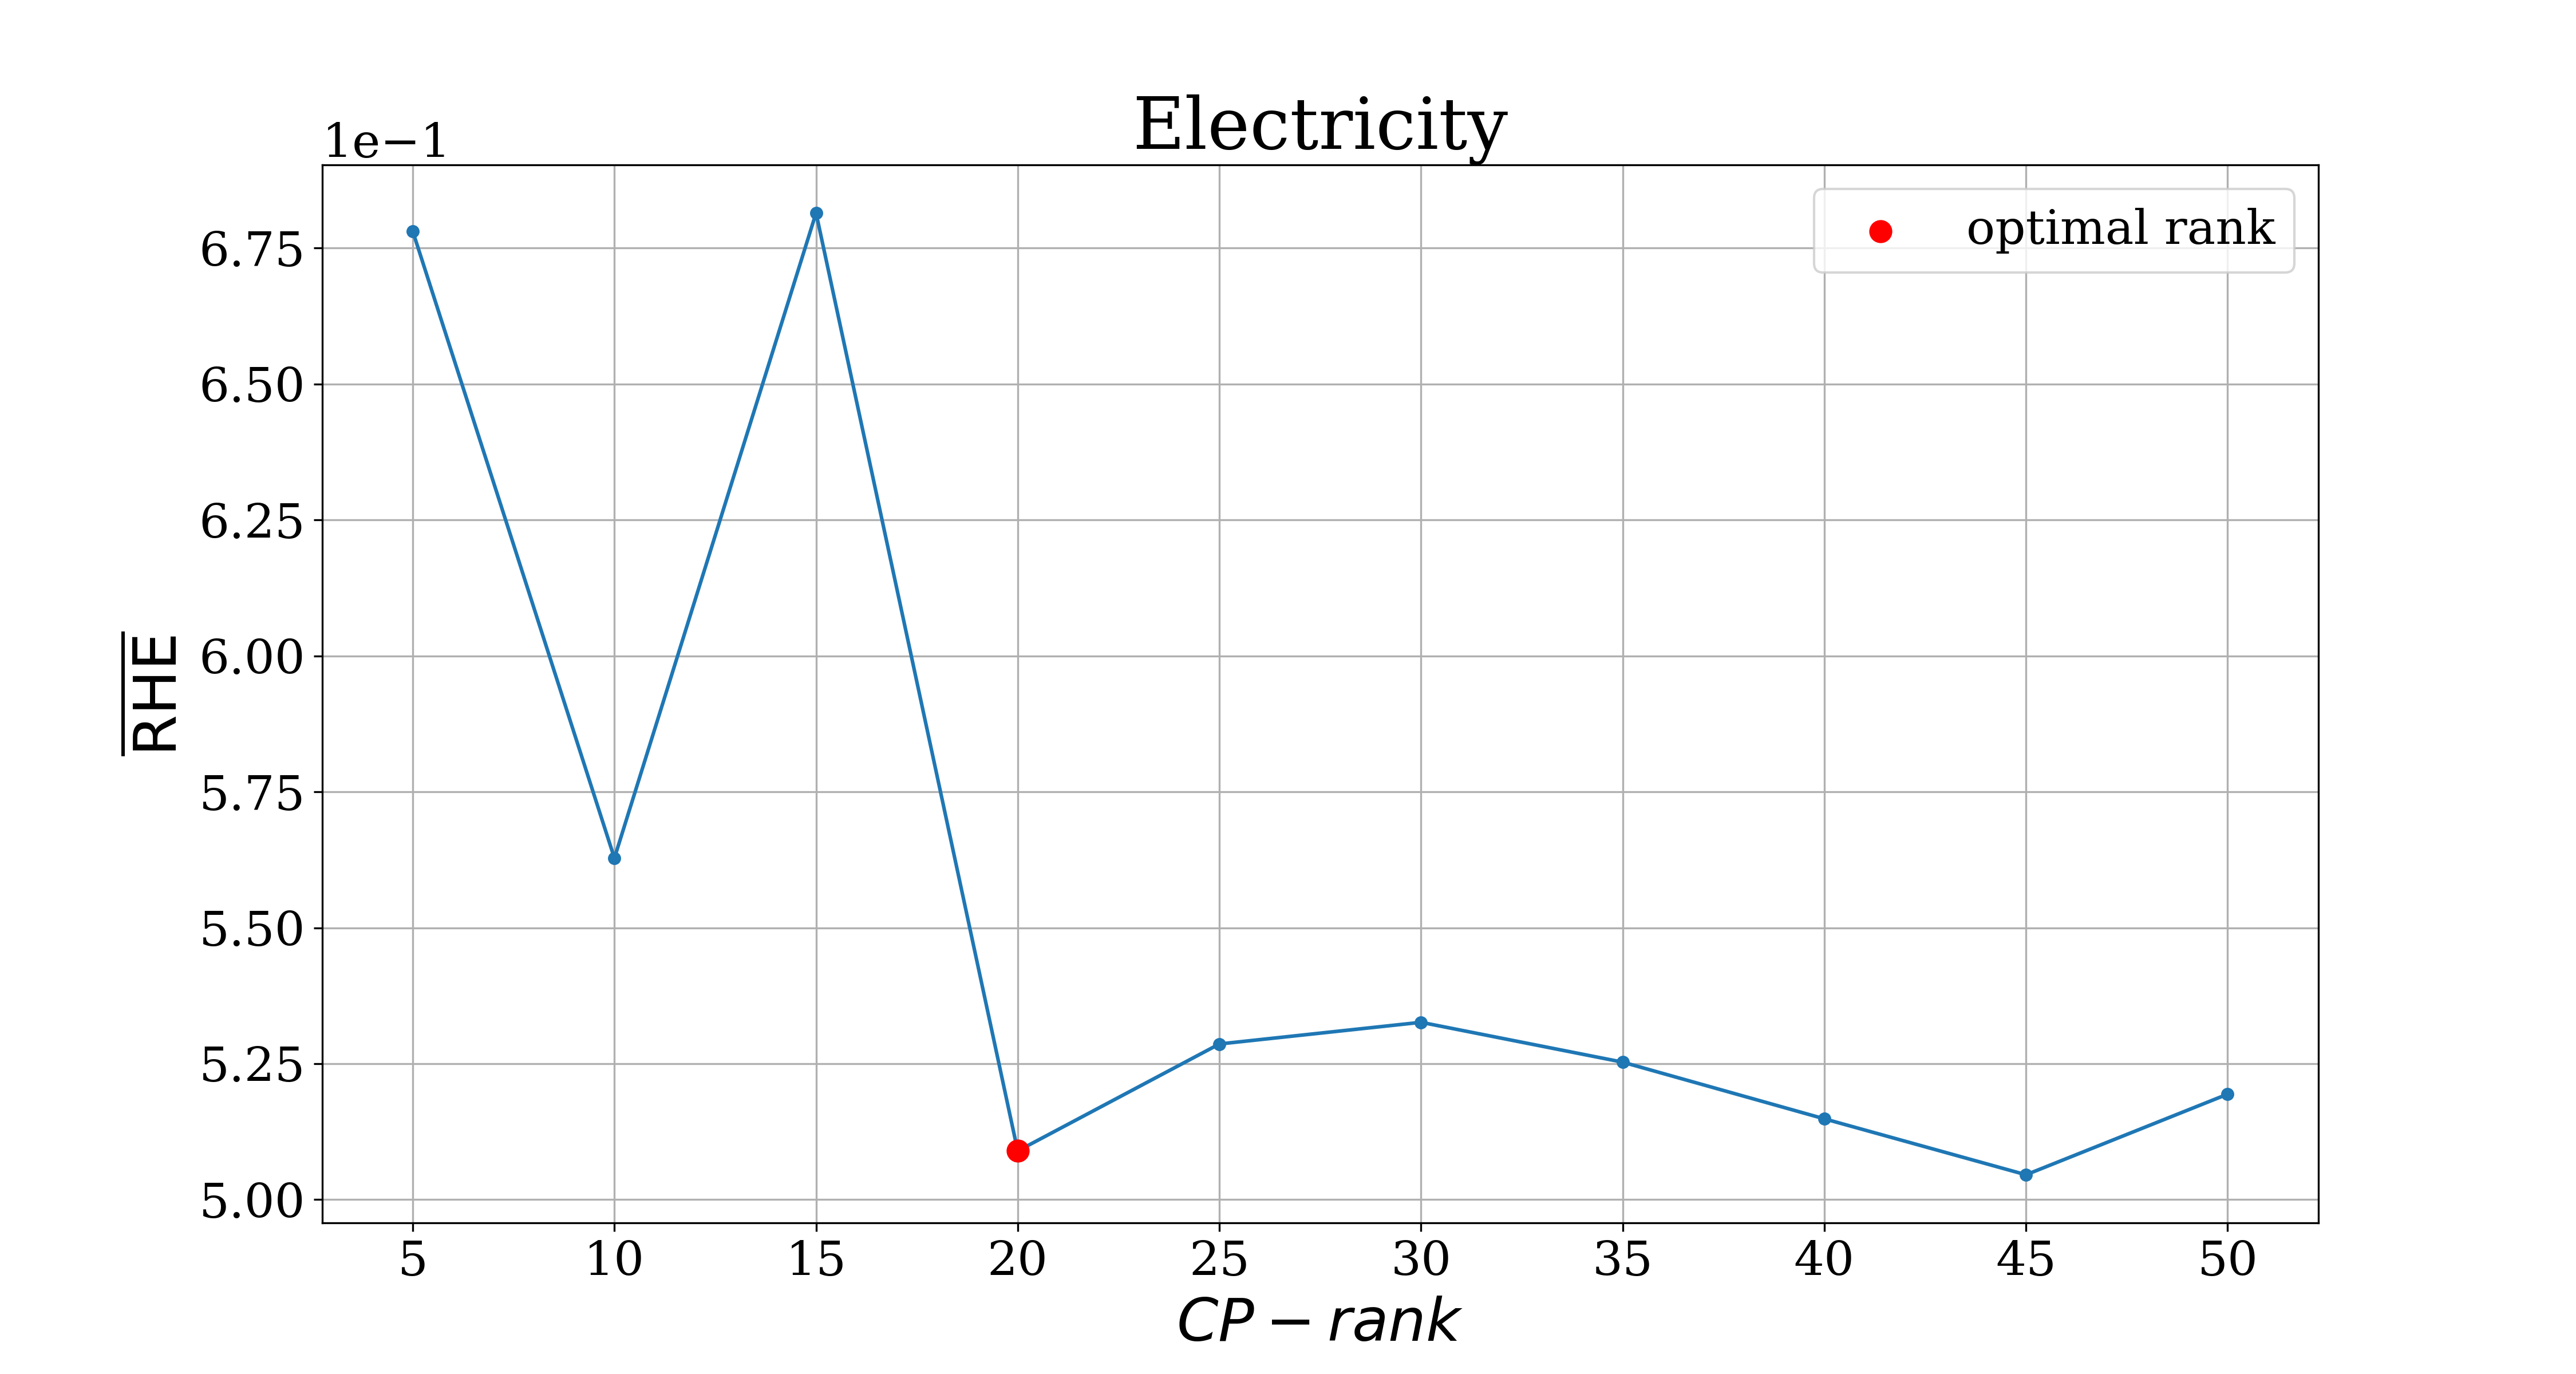
\includegraphics[width=0.33\textwidth, keepaspectratio]{../../experiments/electricity/tssa/figs/decomposition/RHE_mean.png} }
			\subfigure[Данные акселерометрии.]{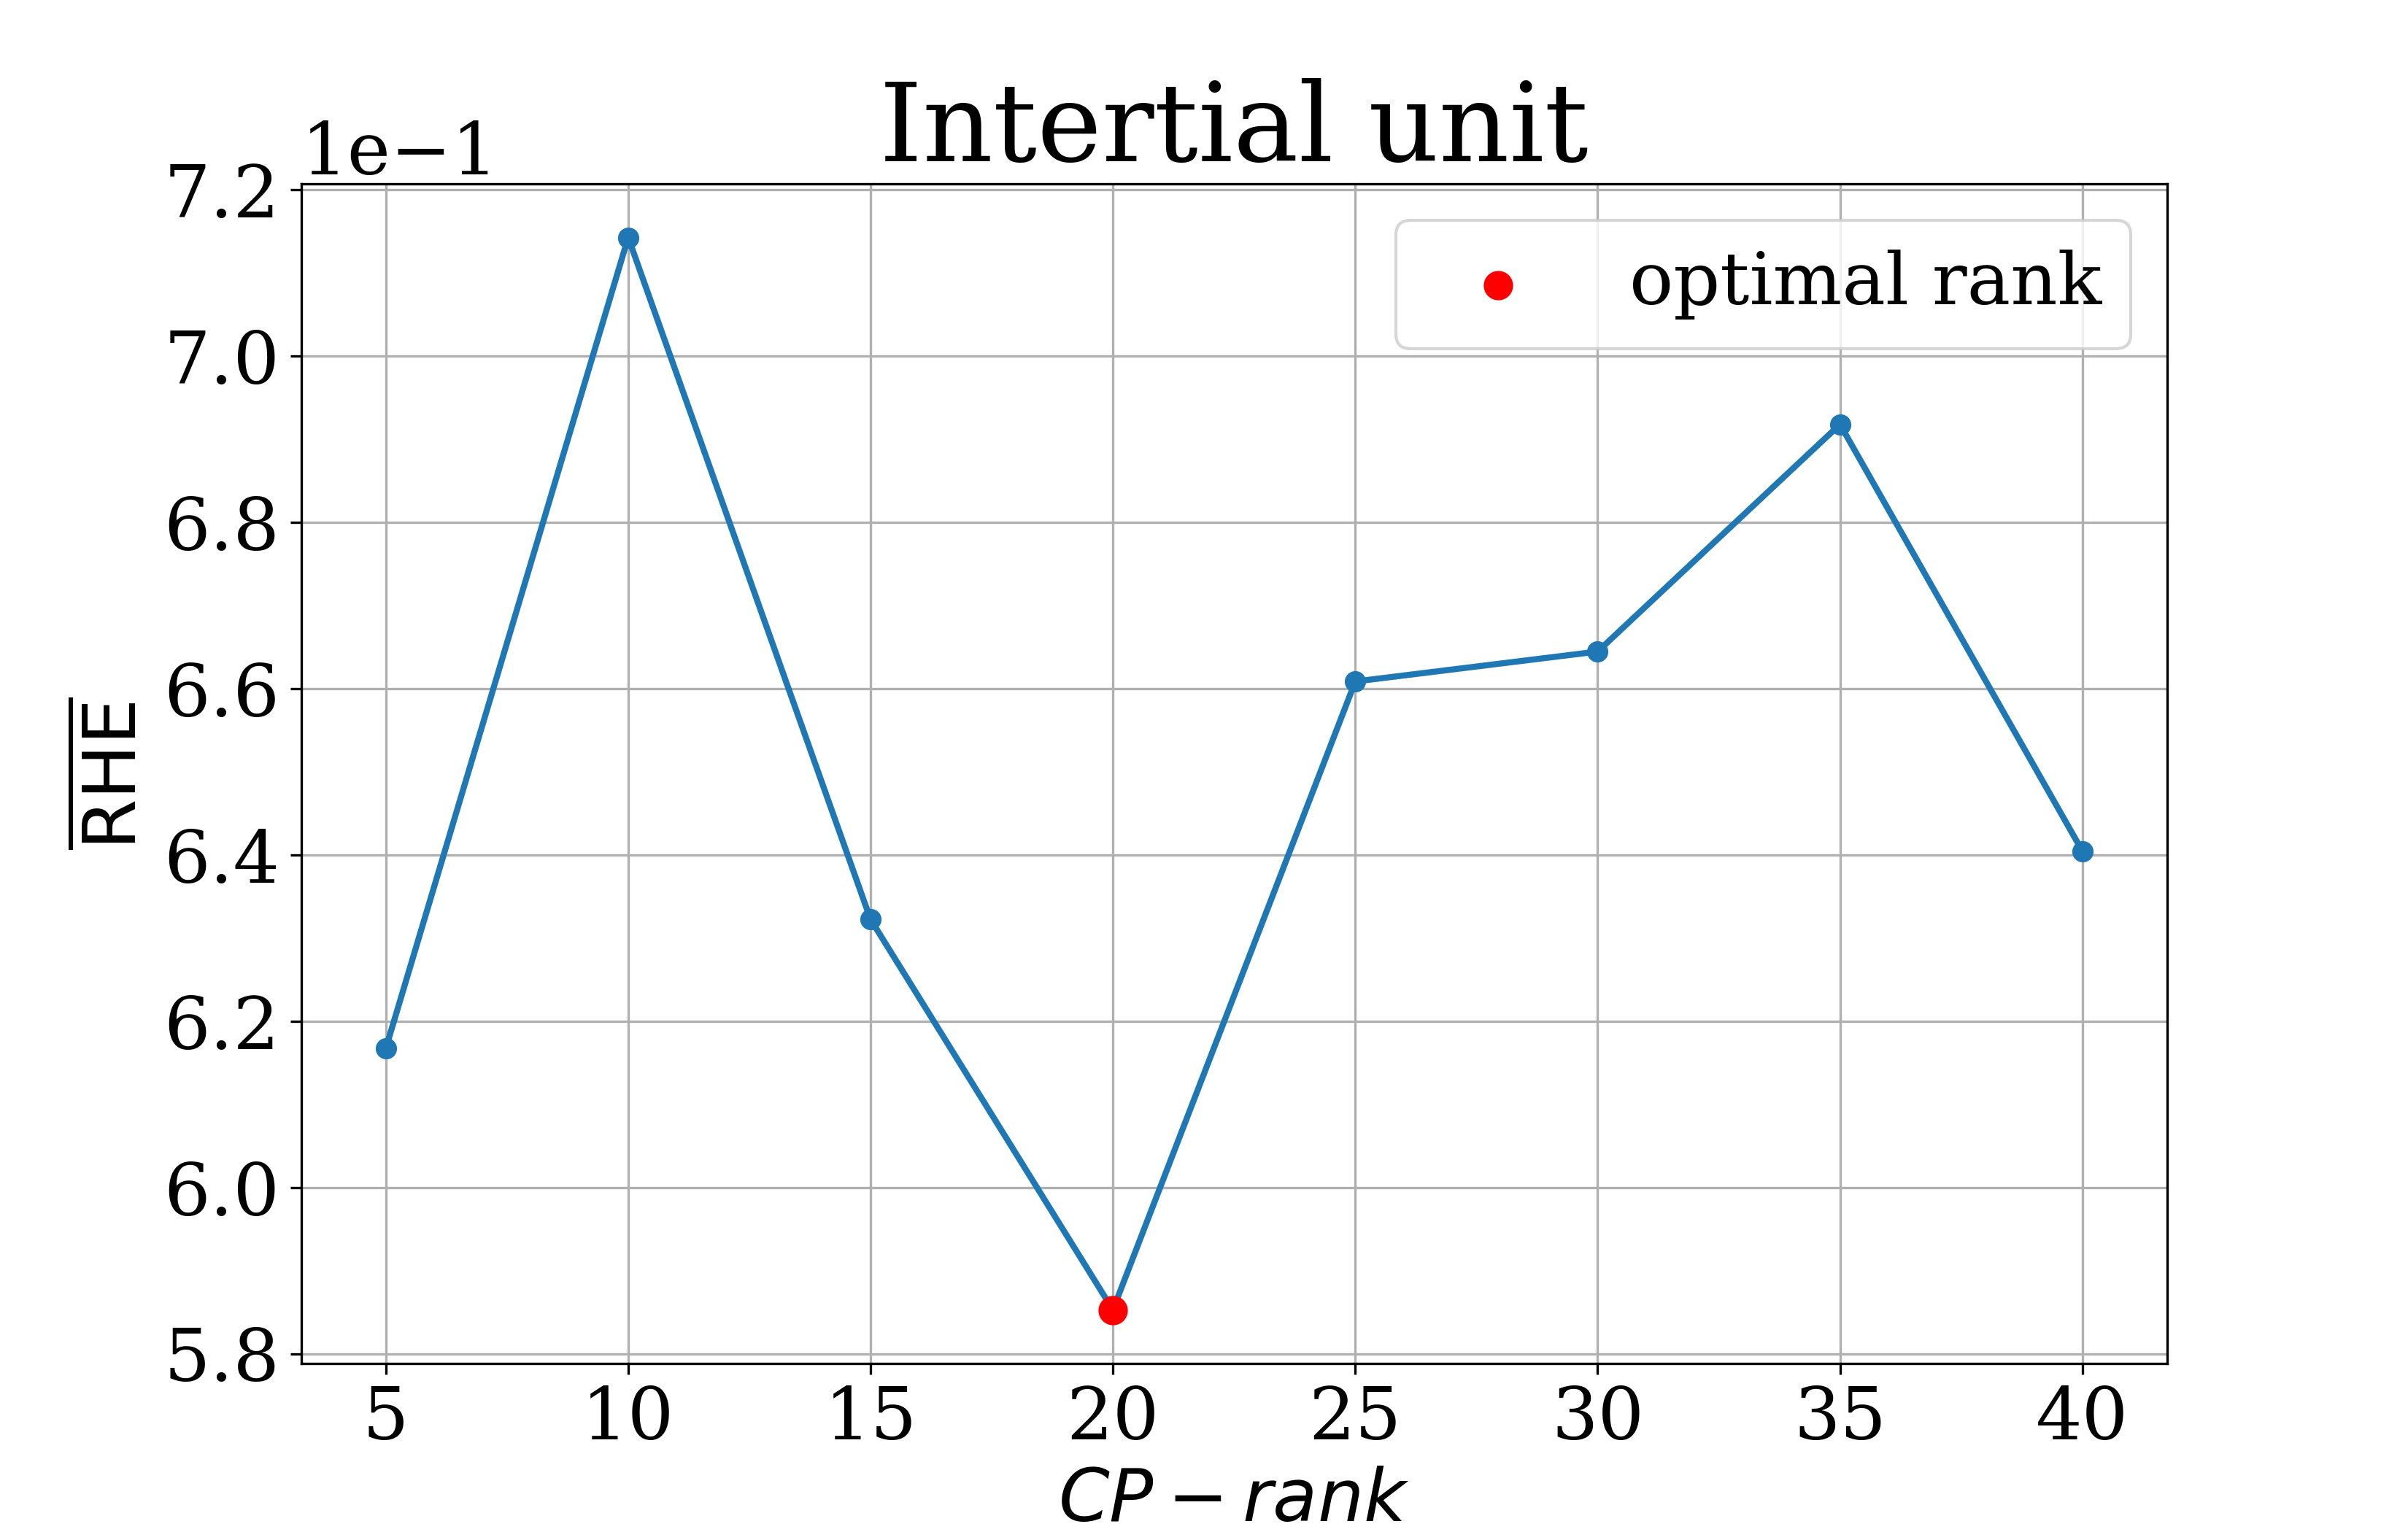
\includegraphics[width=0.33\textwidth, keepaspectratio]{../../experiments/motion_1/tssa/figs/decomposition/RHE_mean.png} }
		\end{figure}
		
		Отдельно выделен оптимальный ранг. Аналогичное падение качества при росте ранга. Разложение на две компоненты:
		
		\begin{center}
			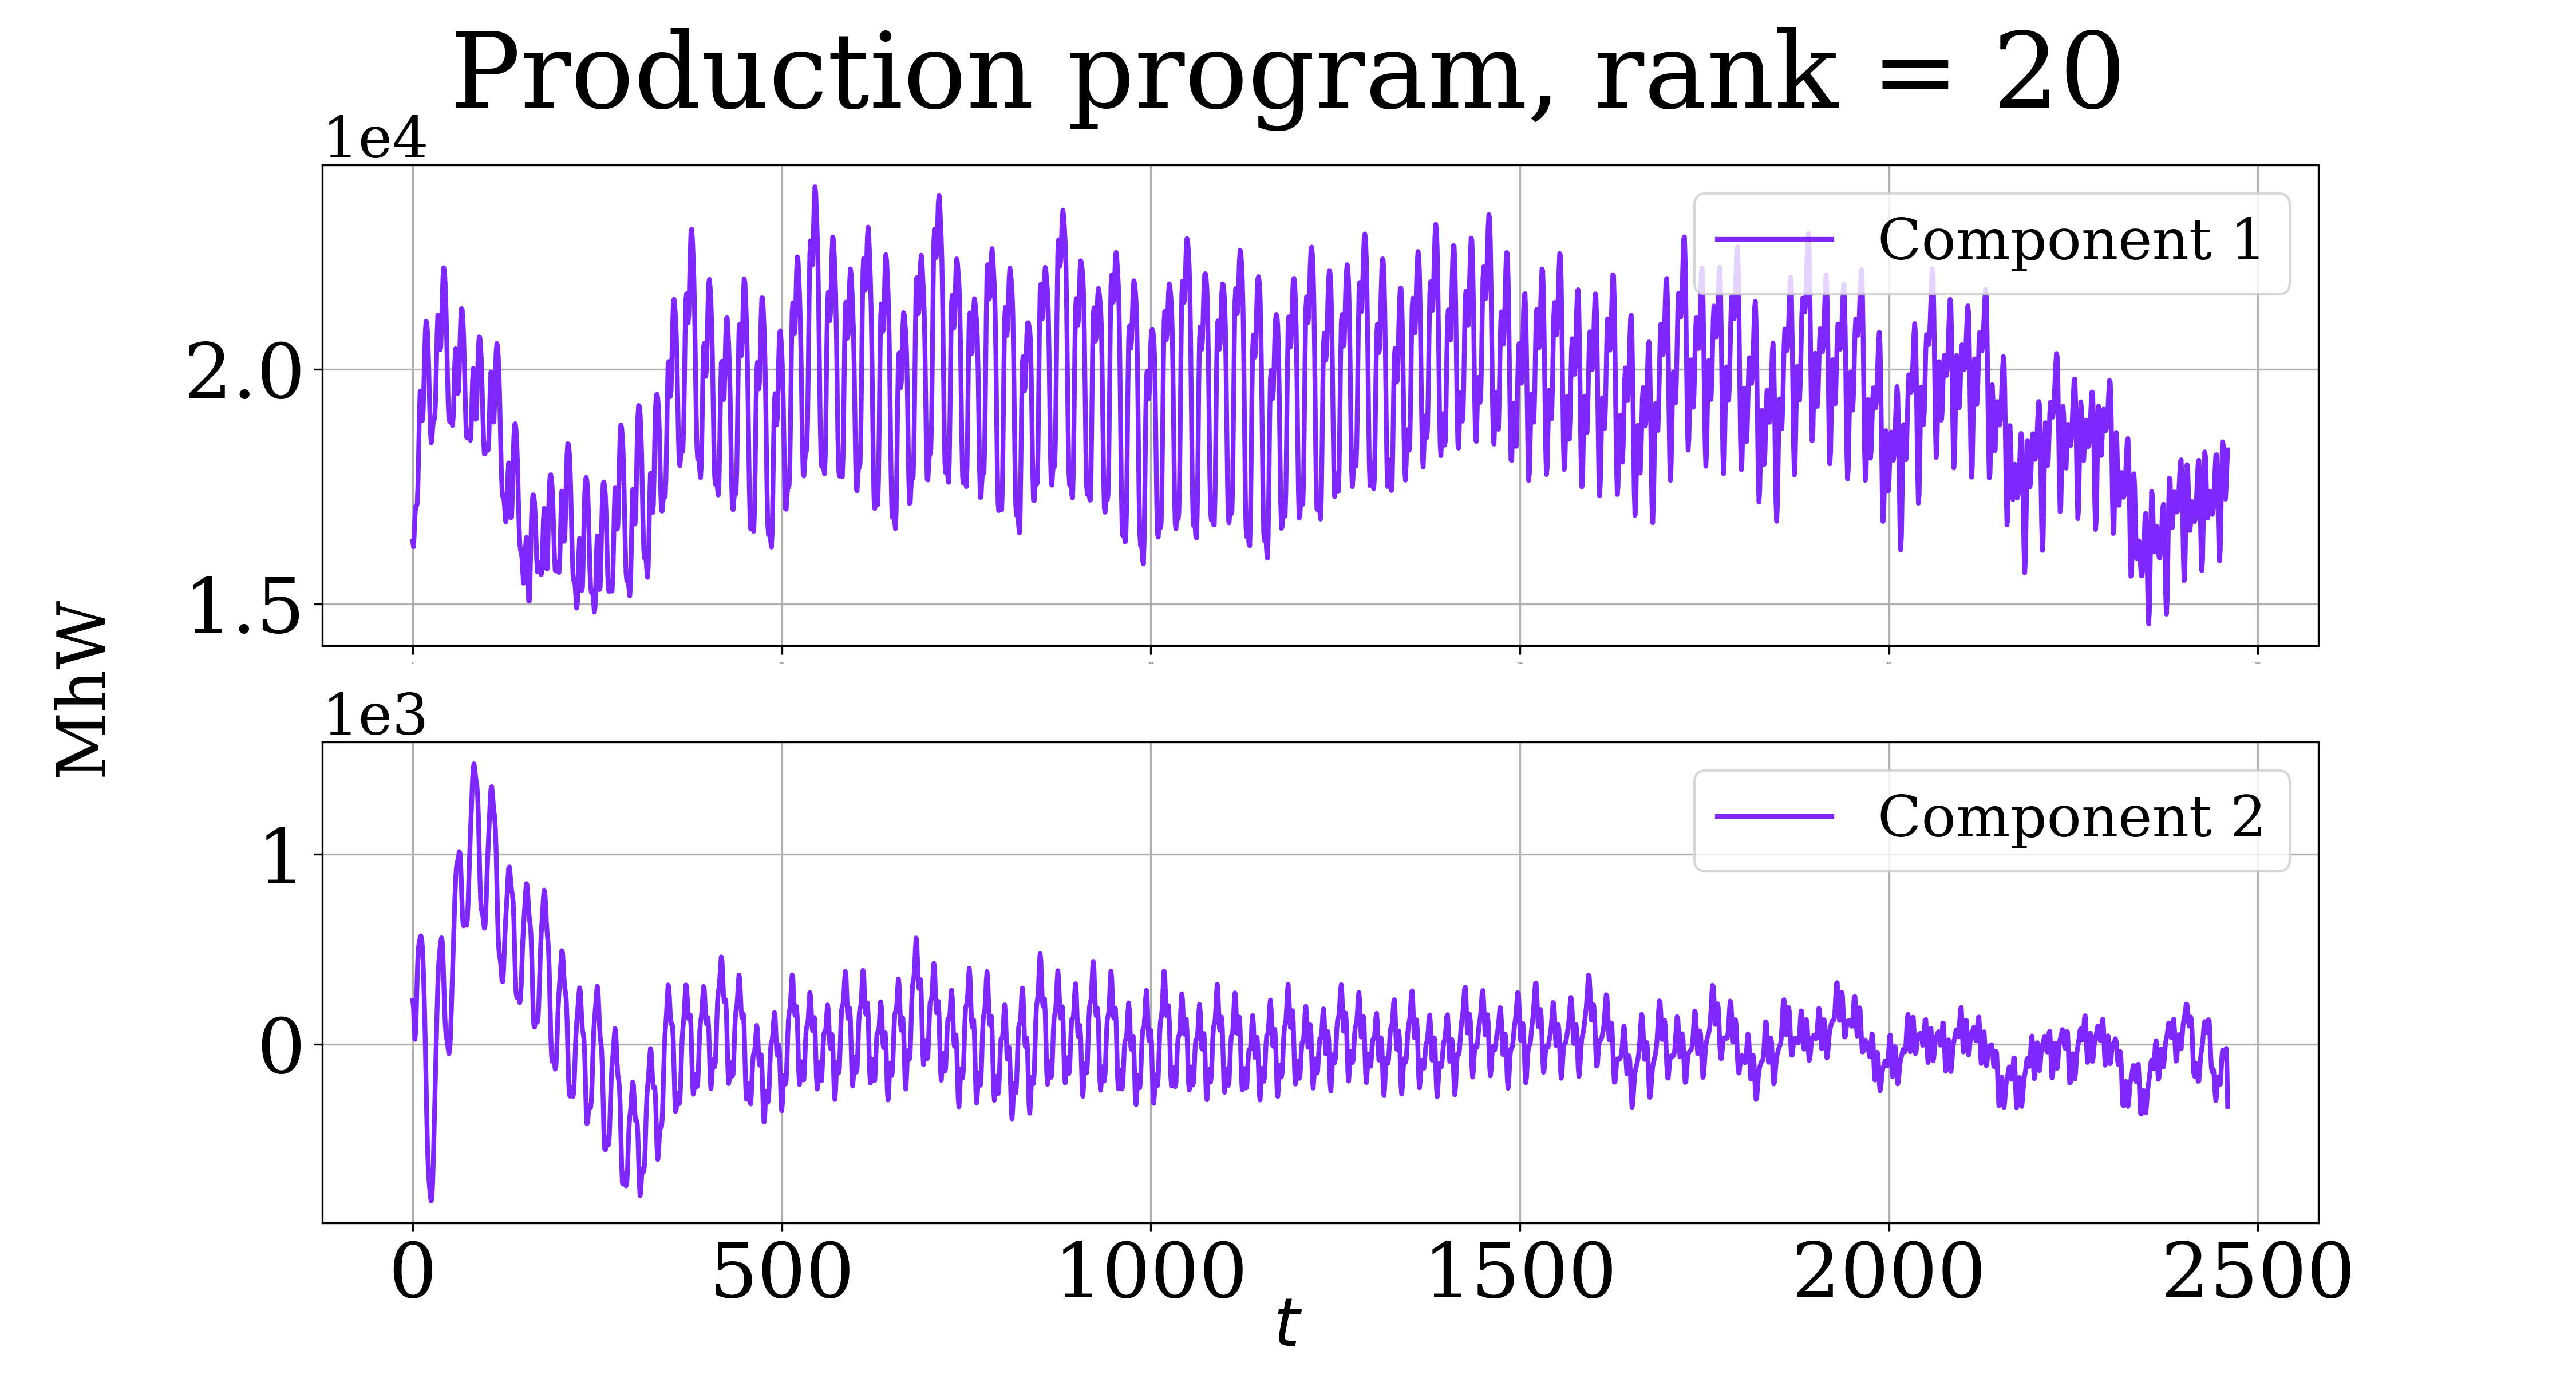
\includegraphics[width=0.43\textwidth, keepaspectratio]{../../experiments/electricity/tssa/figs/decomposition/cpd_rank_20/Production program.png}
			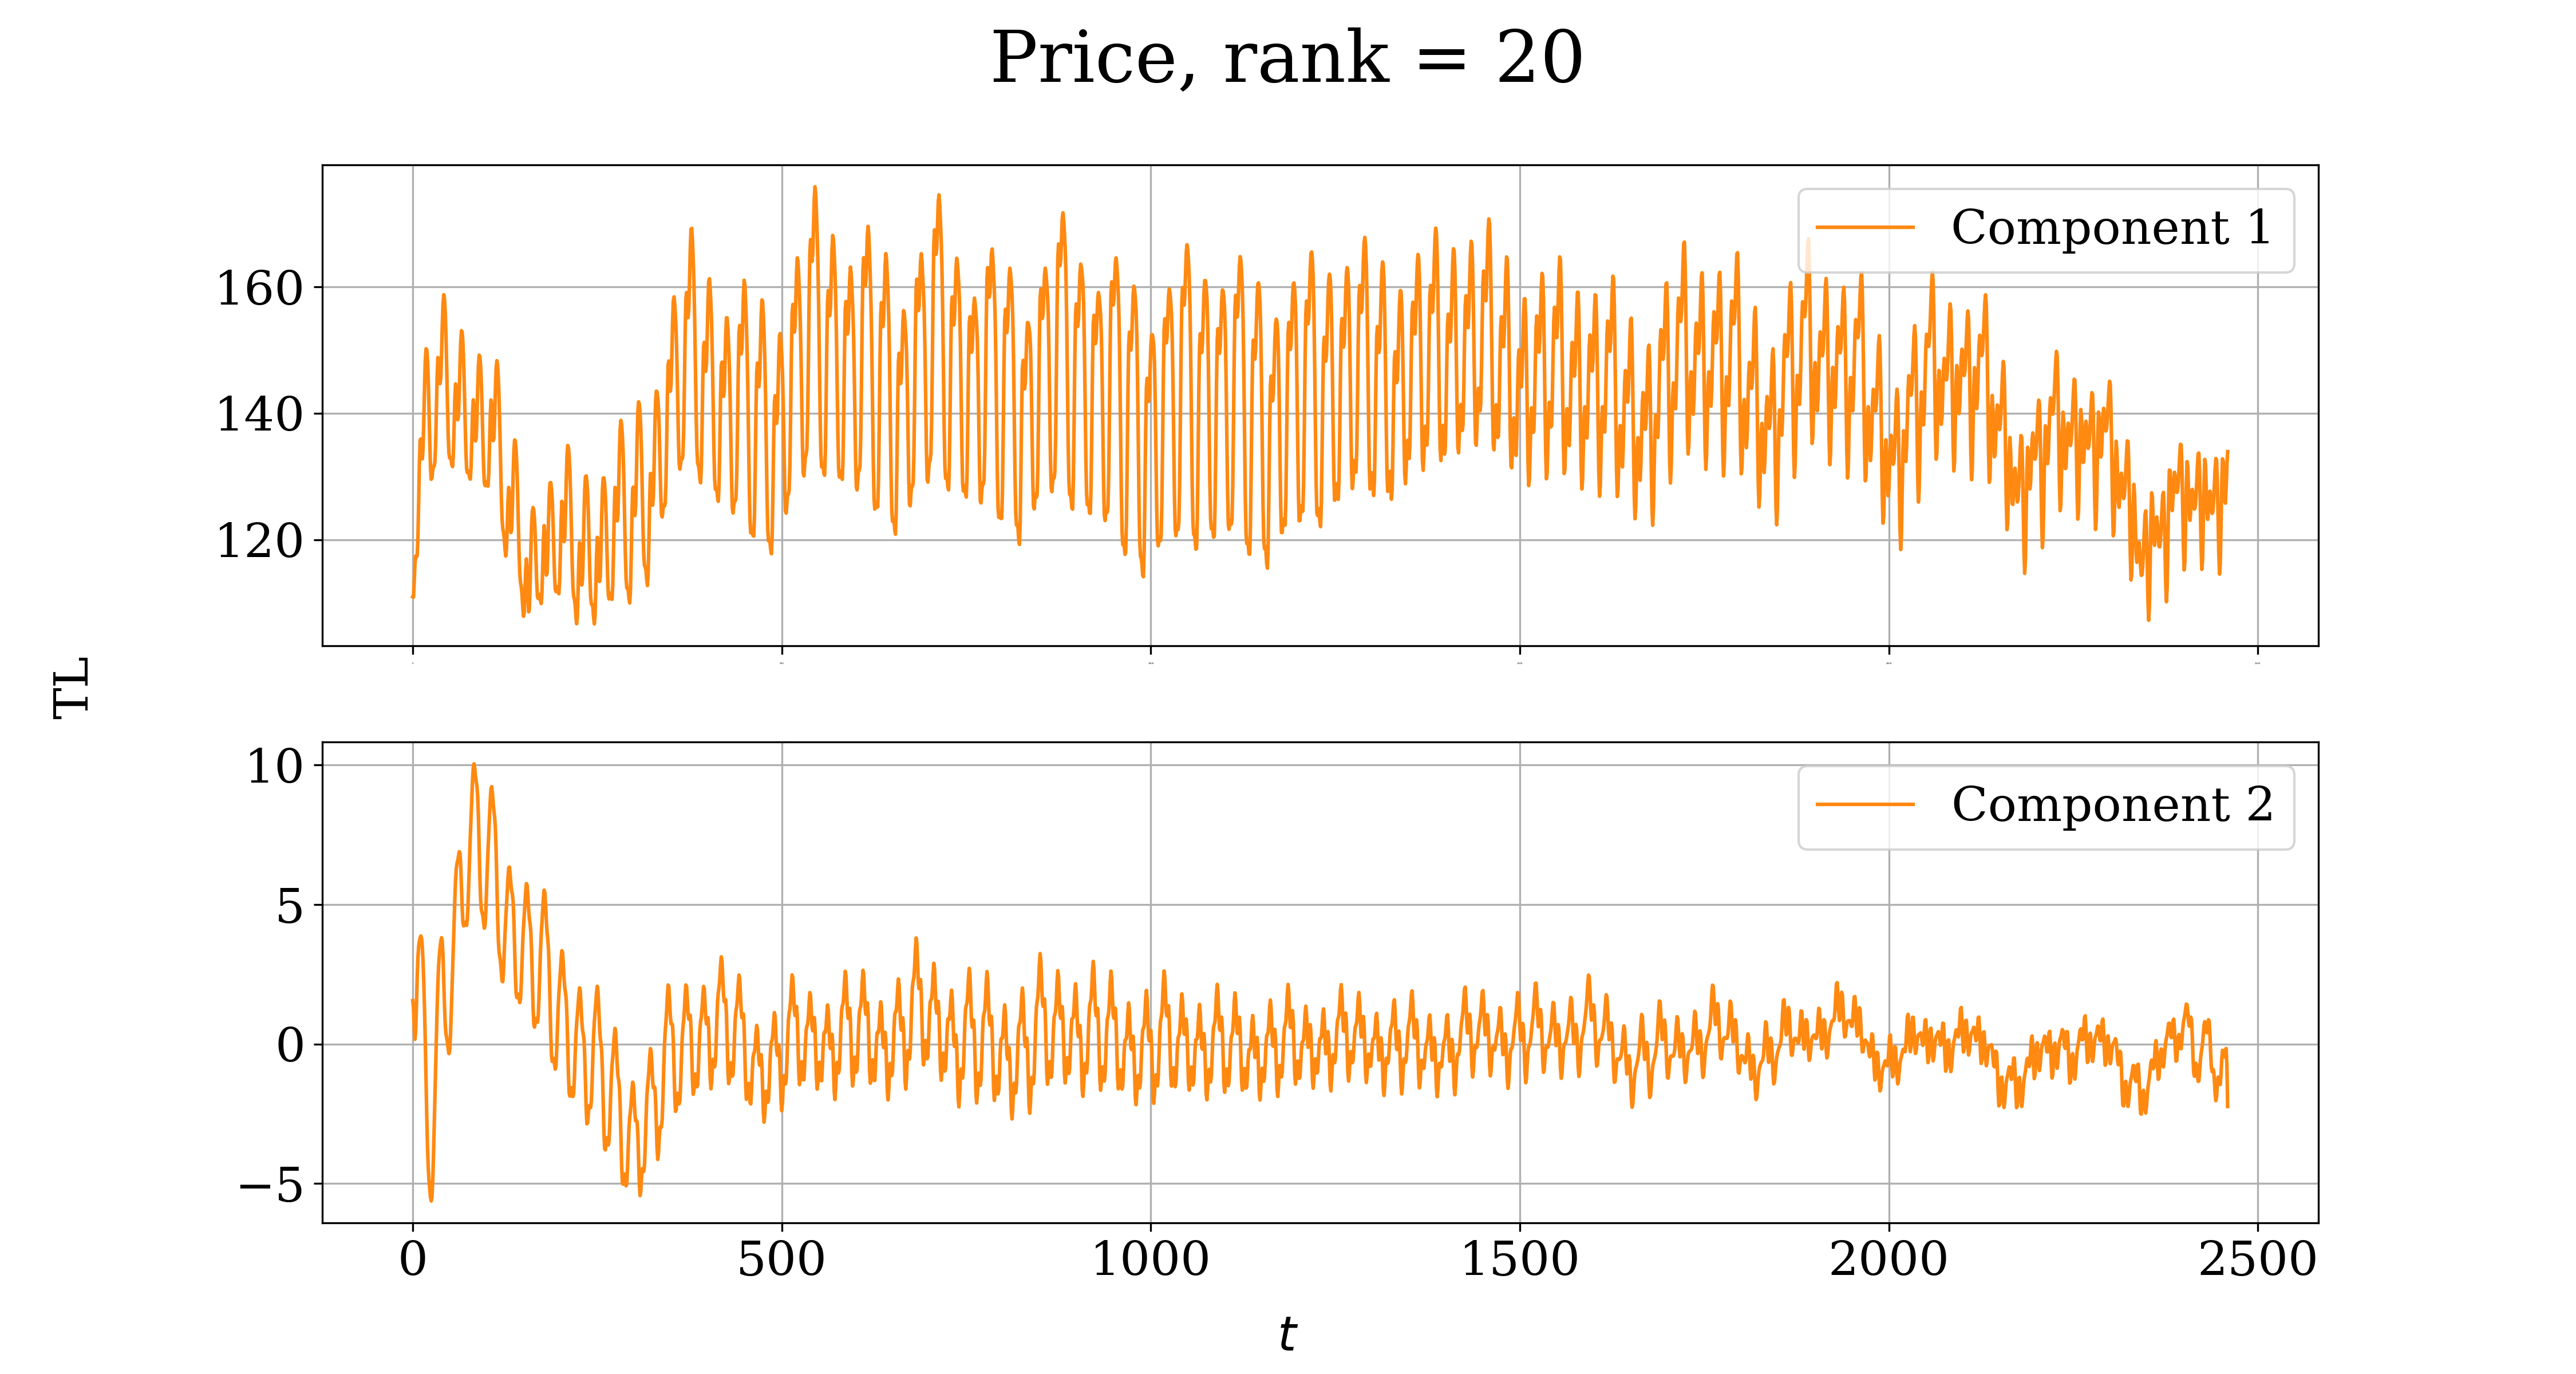
\includegraphics[width=0.43\textwidth, keepaspectratio]{../../experiments/electricity/tssa/figs/decomposition/cpd_rank_20/Price.png} \\
			{\small Данные электроэнергии.} \\
		\end{center}
		
	\end{frame}
	
	\begin{frame}{Визуализация компонент разложения tSSA}
		
		\begin{center}
			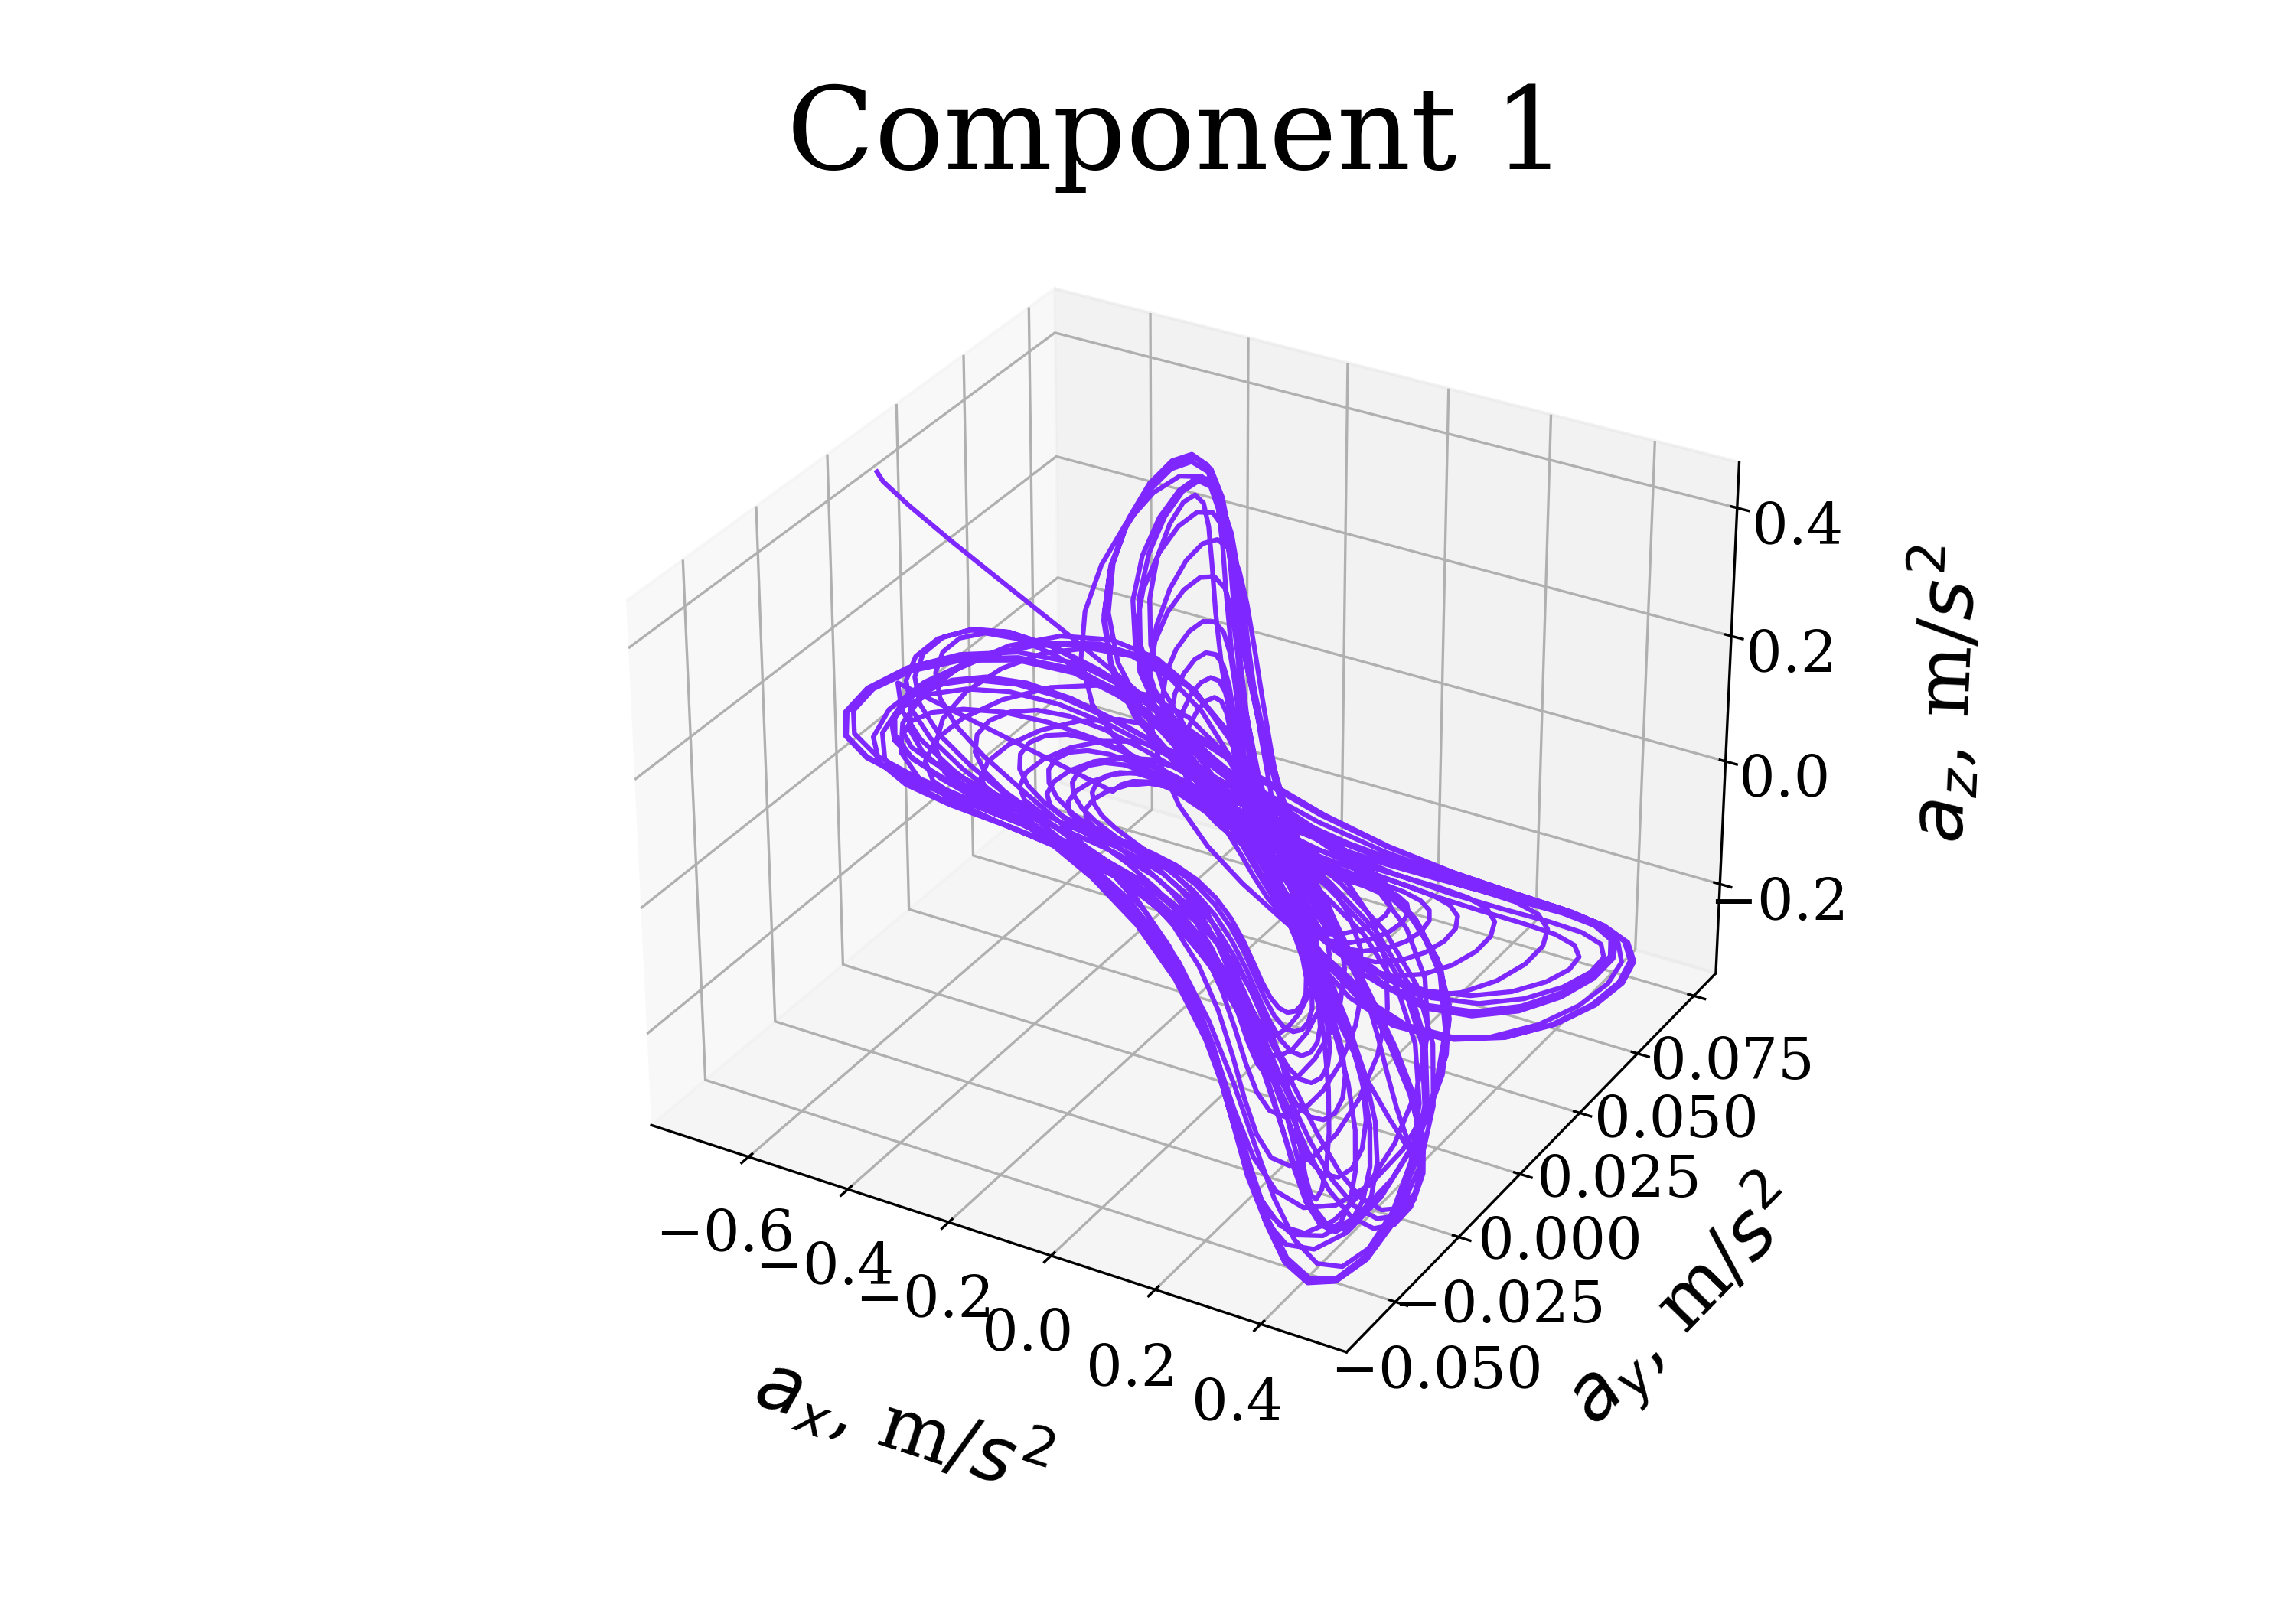
\includegraphics[width=0.35\textwidth, keepaspectratio]{../../experiments/motion_1/tssa/figs/decomposition/cpd_rank_15/acceler_1.png}
			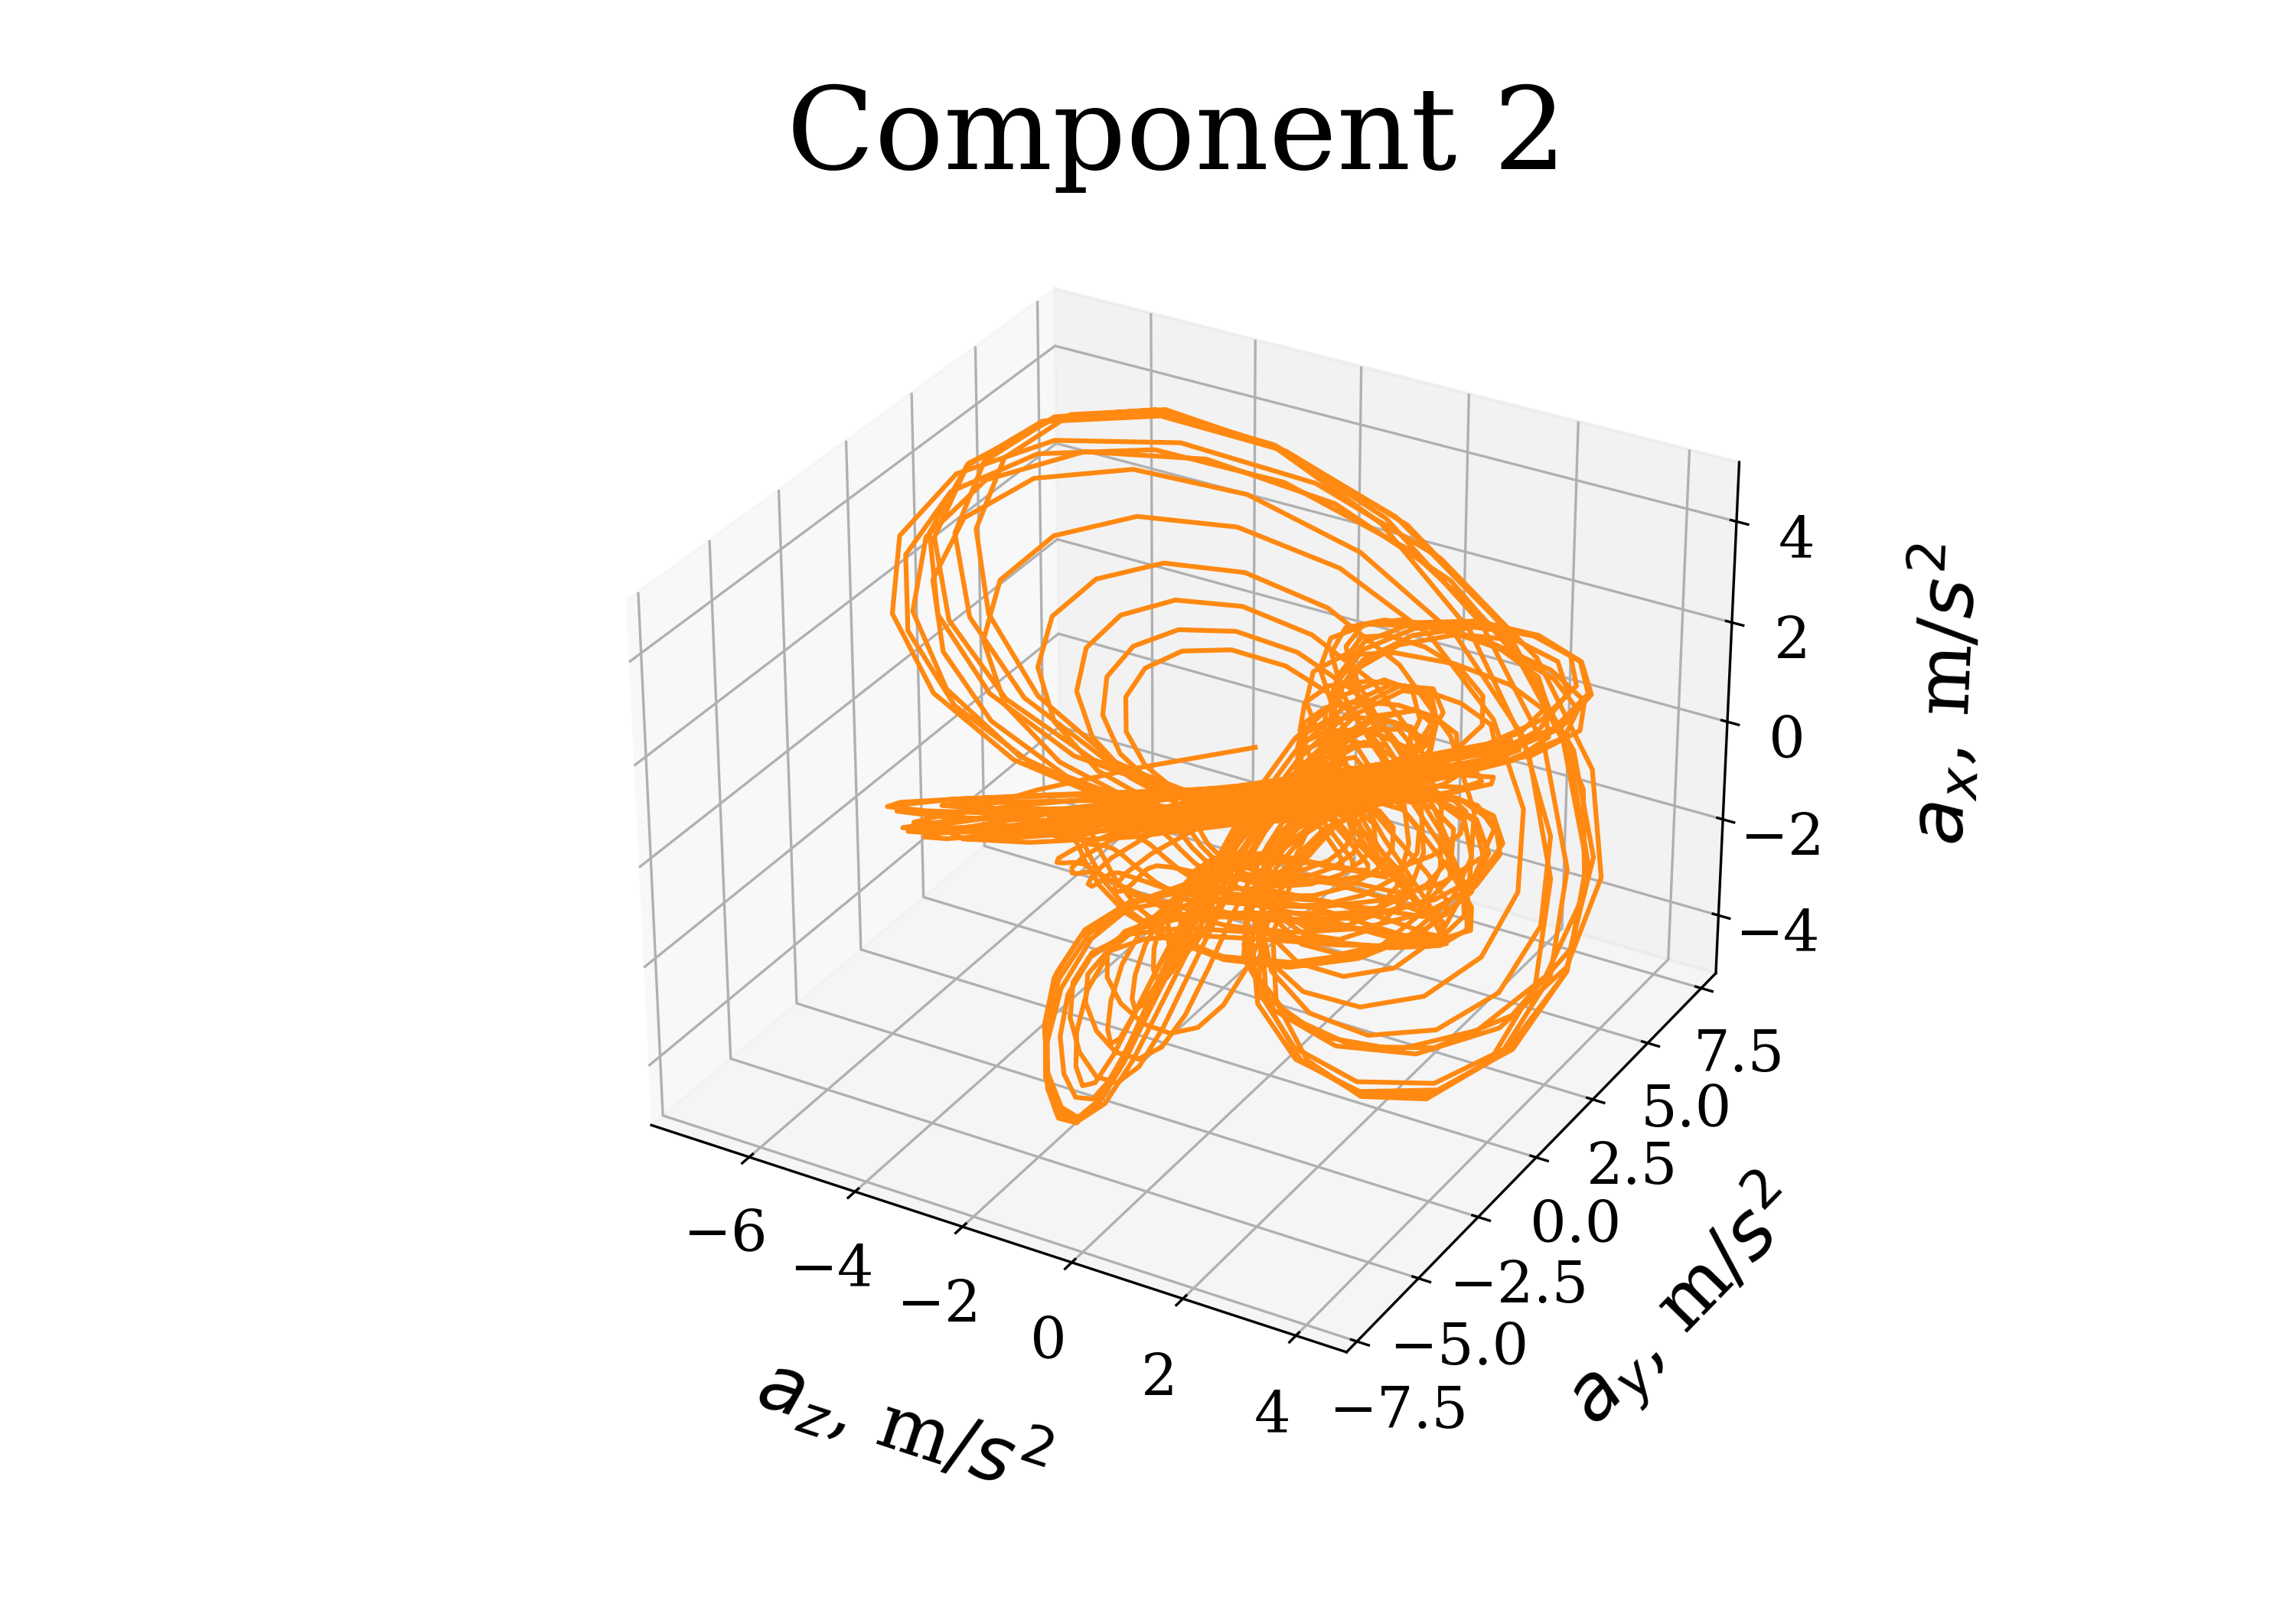
\includegraphics[width=0.35\textwidth, keepaspectratio]{../../experiments/motion_1/tssa/figs/decomposition/cpd_rank_15/acceler_2.png} \\
			{\small Данные акселерометра.} \\
			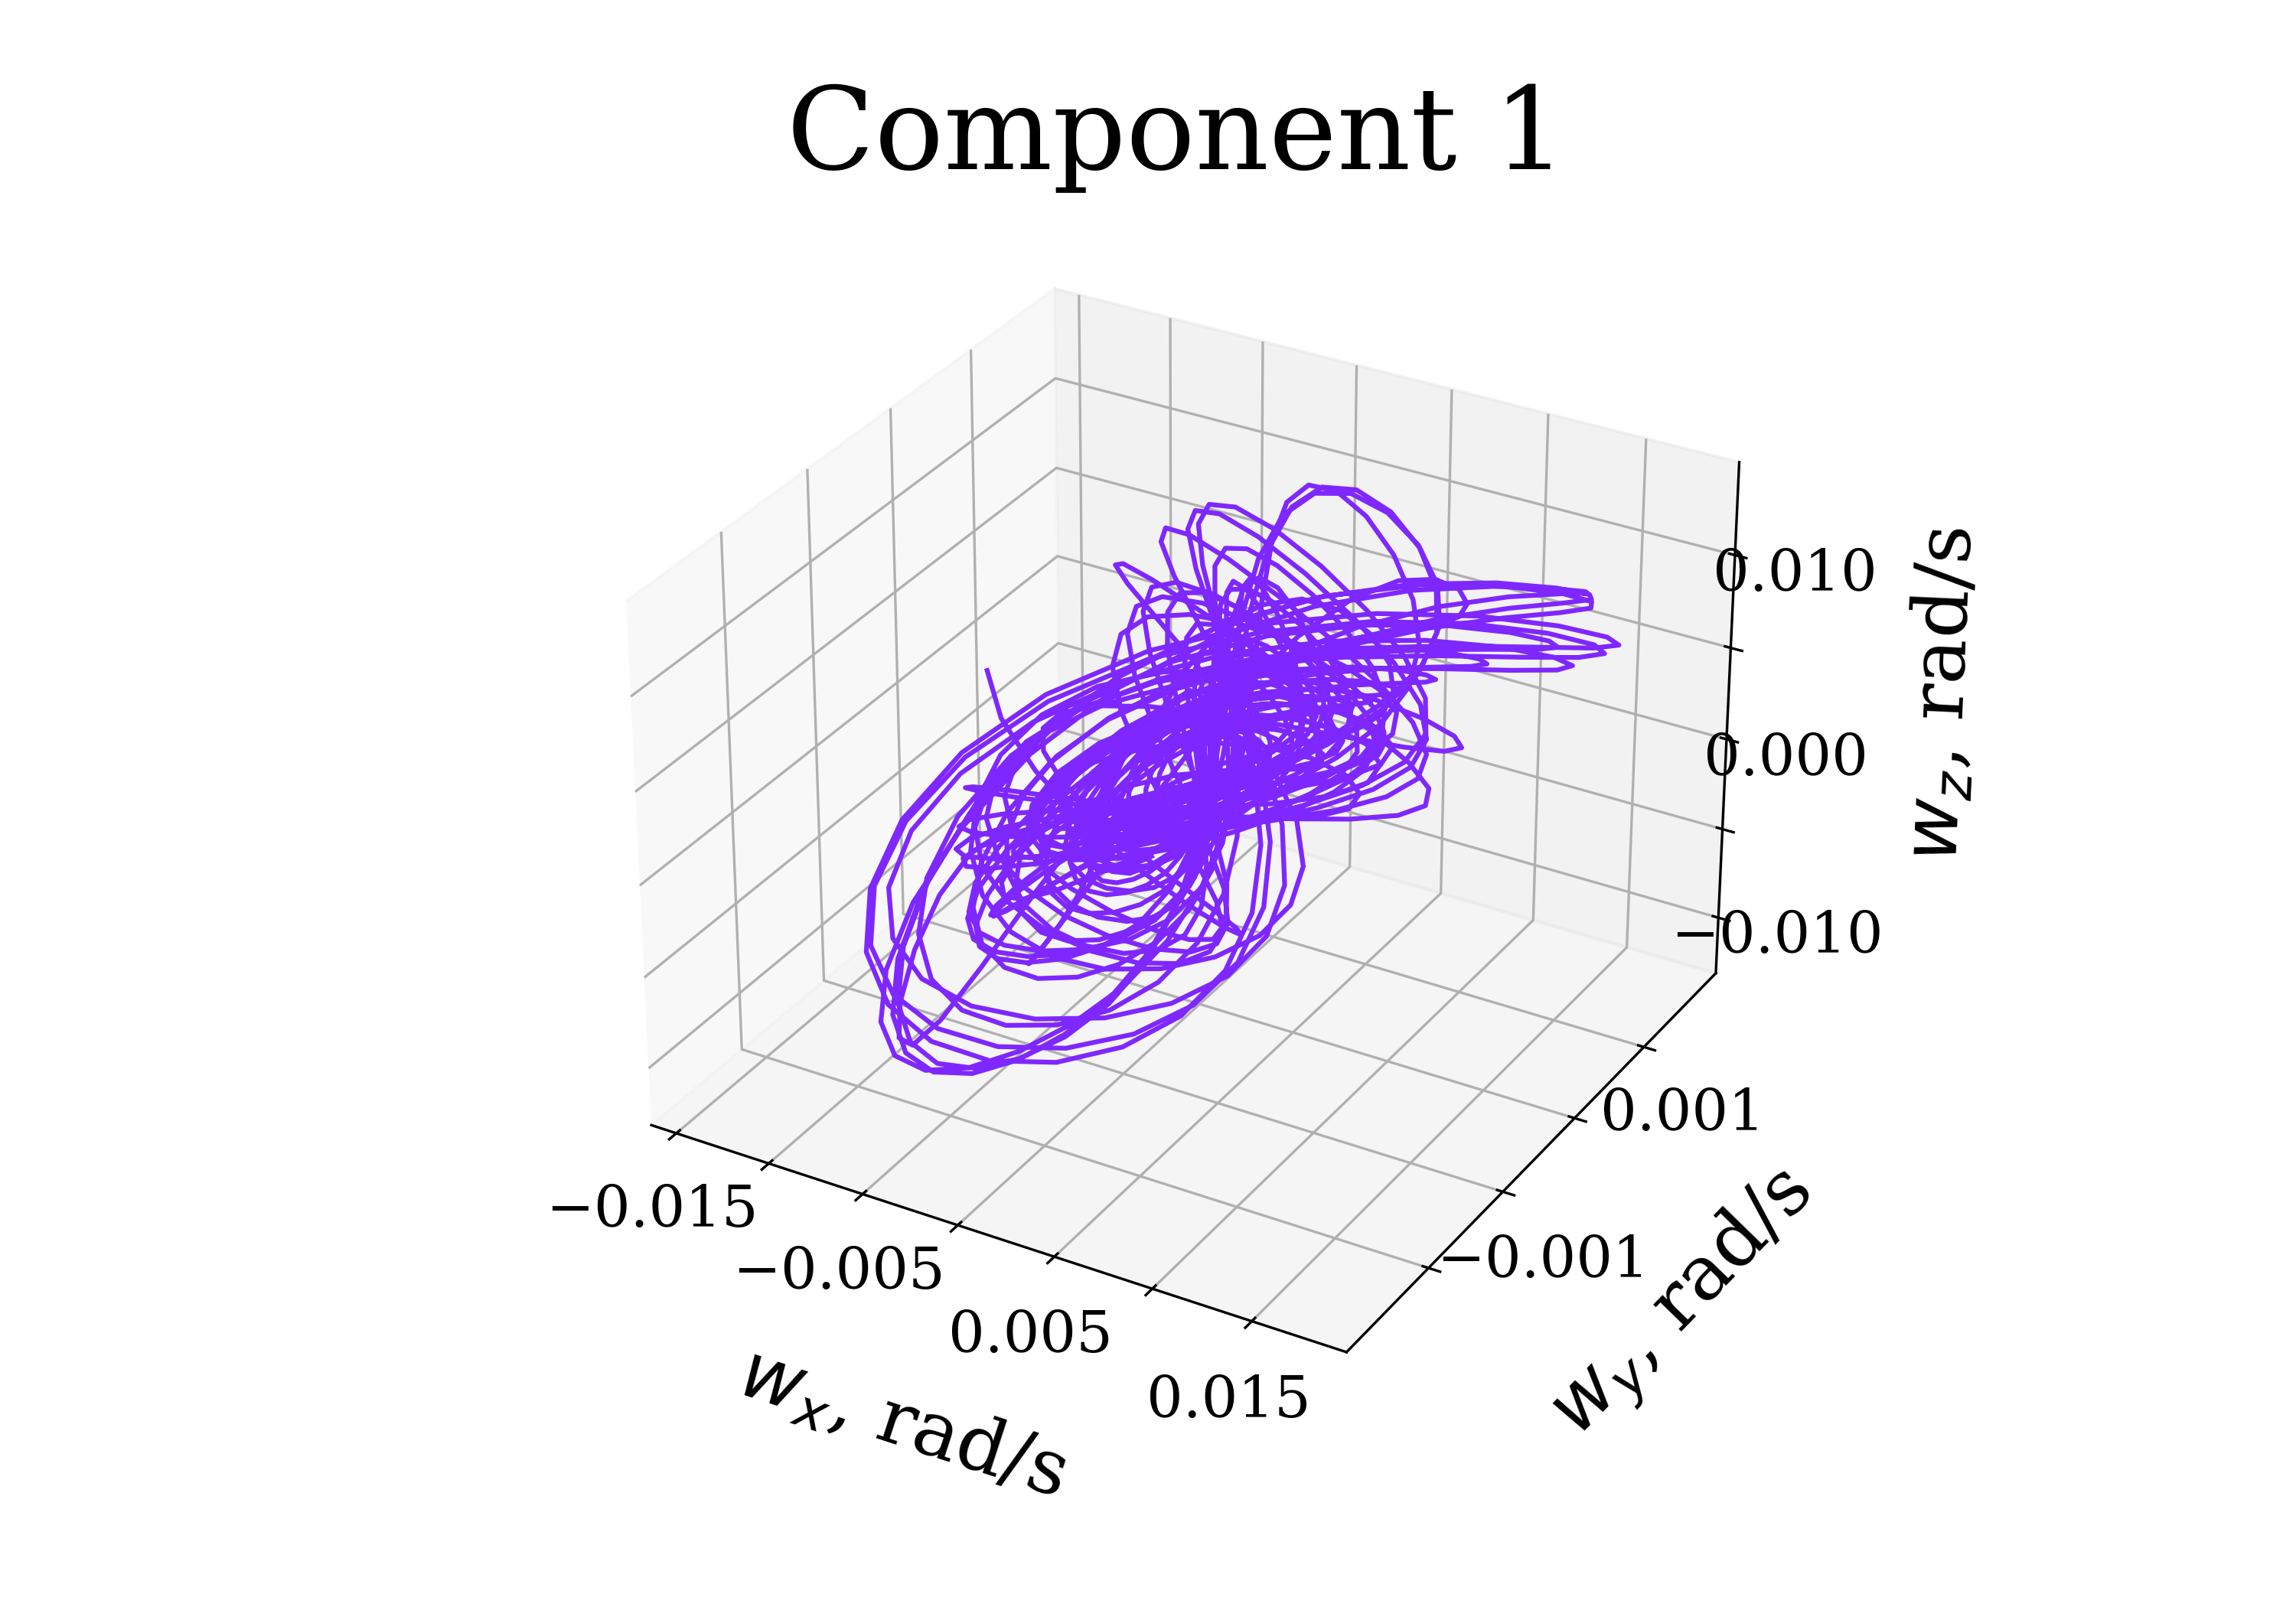
\includegraphics[width=0.35\textwidth, keepaspectratio]{../../experiments/motion_1/tssa/figs/decomposition/cpd_rank_15/gyro_1.png}
			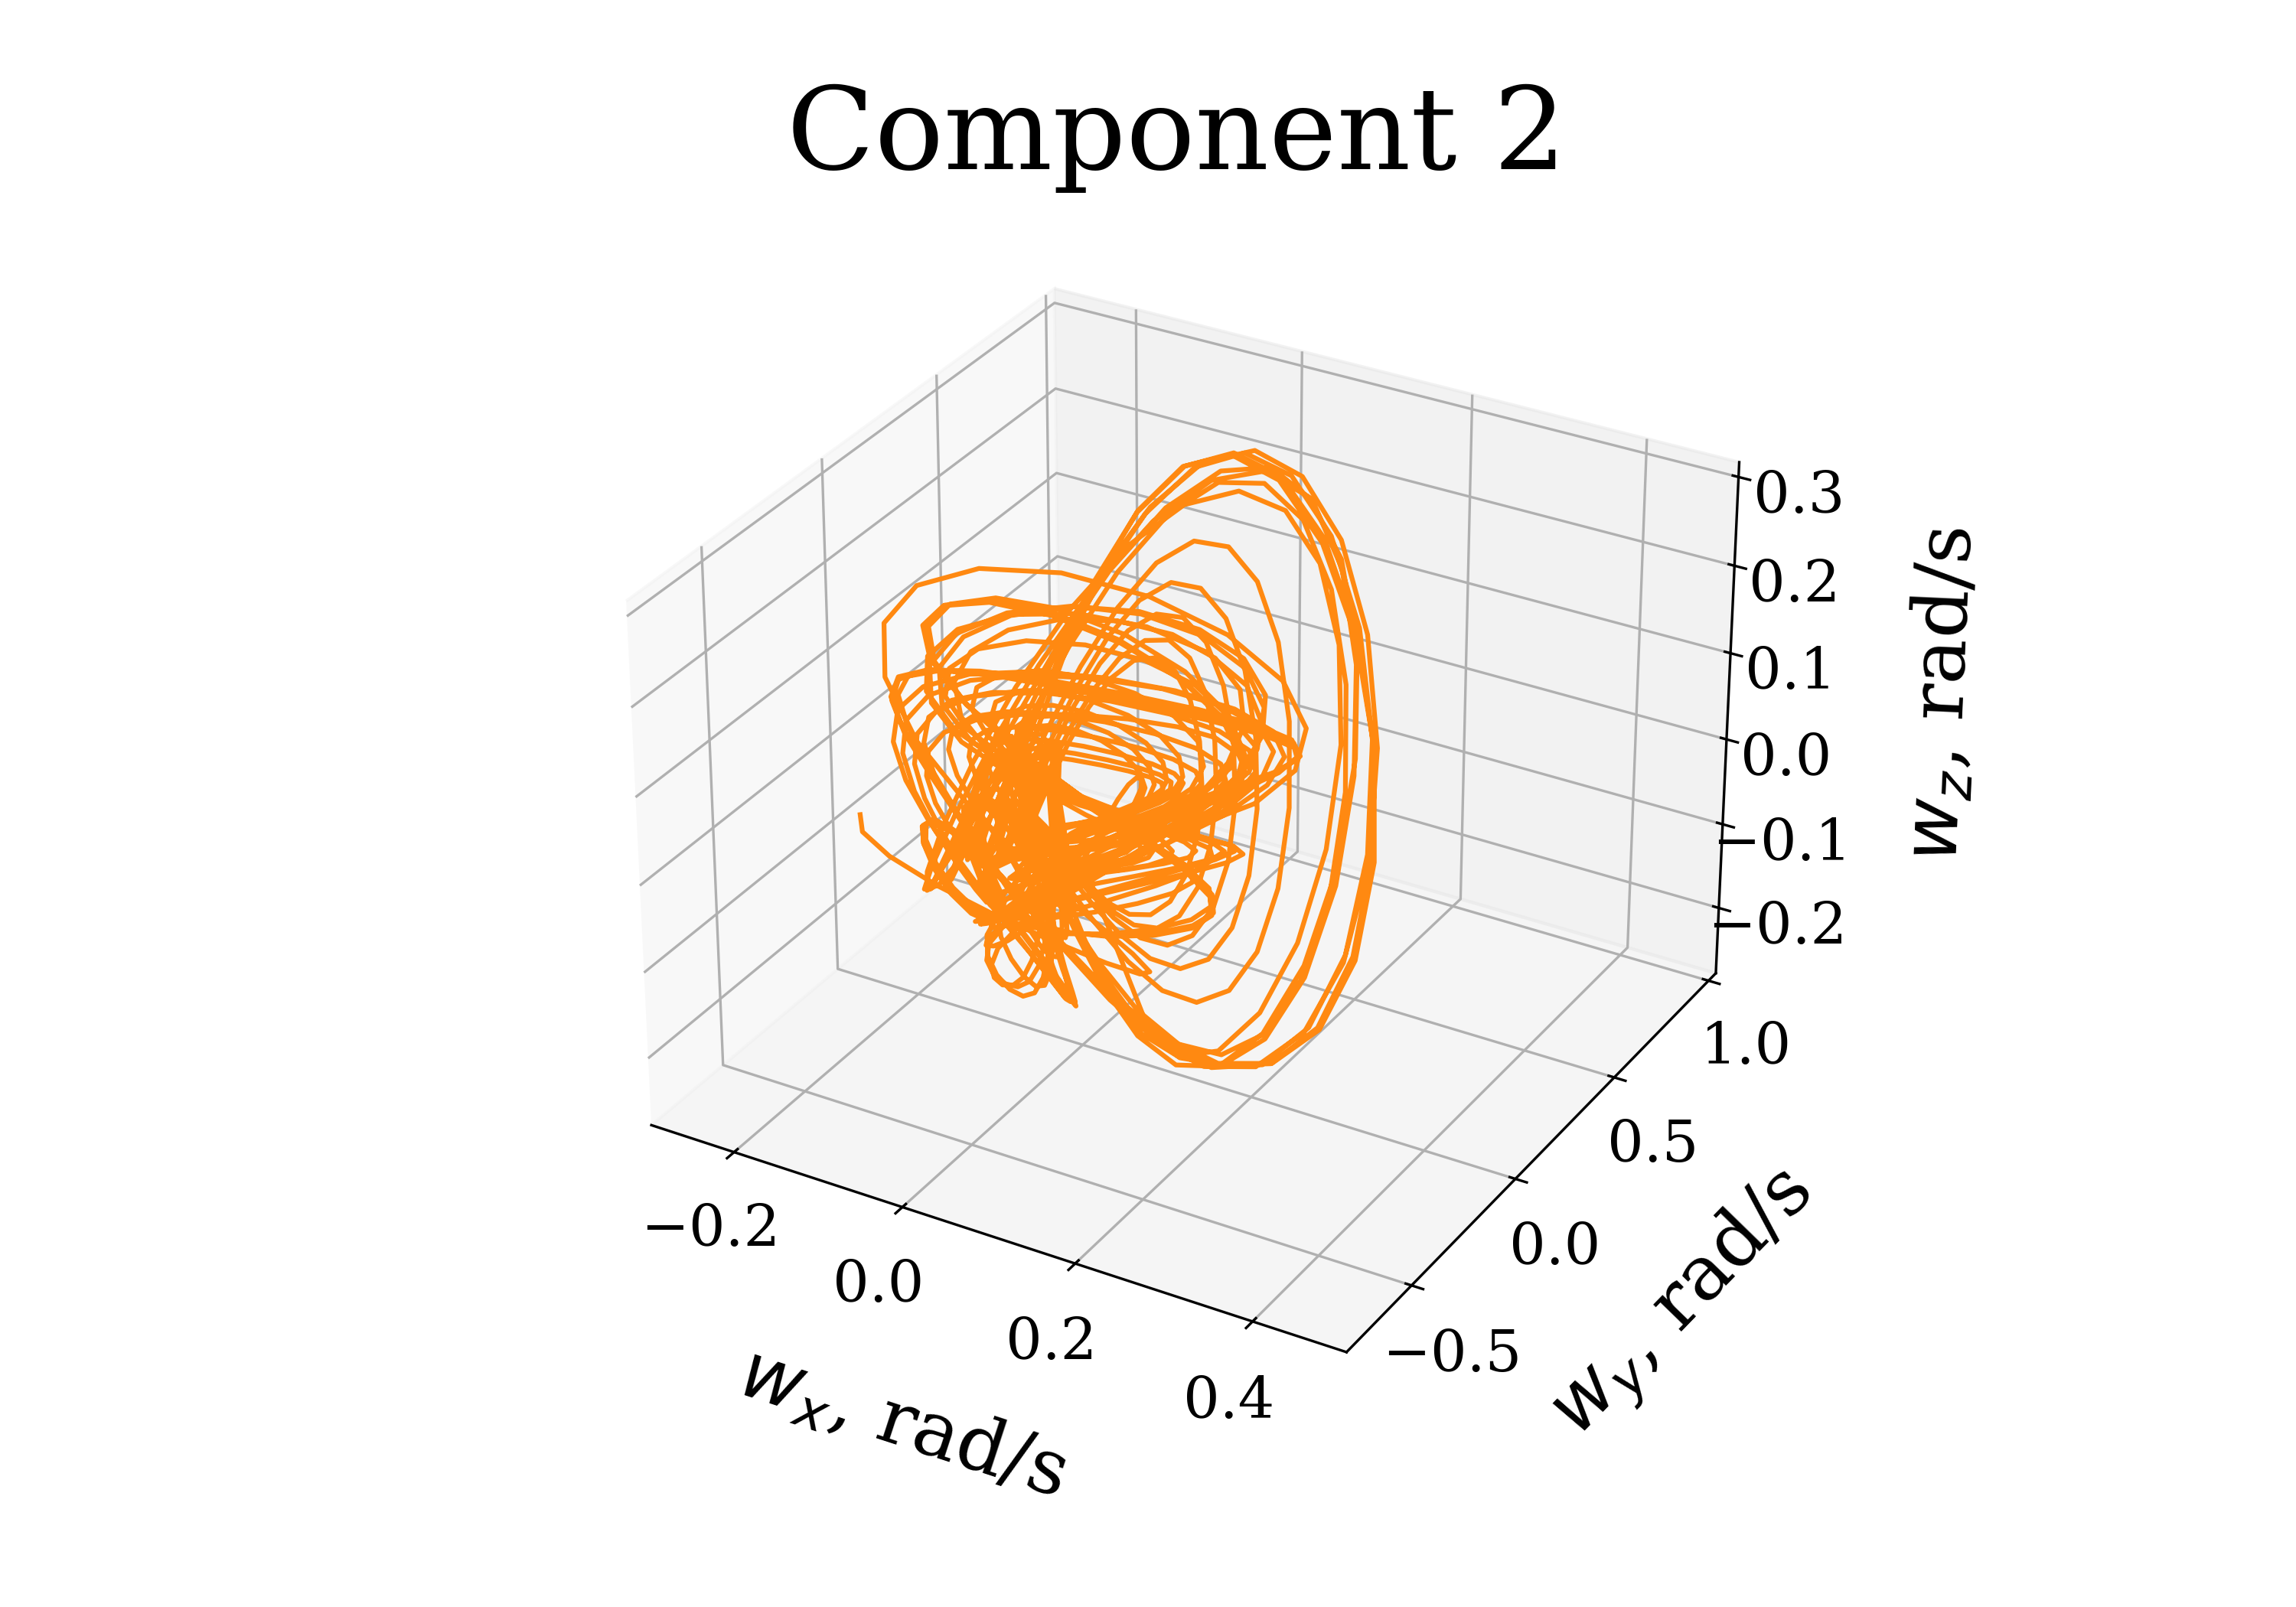
\includegraphics[width=0.35\textwidth, keepaspectratio]{../../experiments/motion_1/tssa/figs/decomposition/cpd_rank_15/gyro_2.png} \\
			{\small Данные гироскопа.} \\
		\end{center}
		
		Компоненты наглядно показывают эффект общего базиса сигналов, а также нетривиальную динамику порождения данных.
		
	\end{frame}
	
	\begin{frame}{Качество декомпозиции моделей}
		
		\begin{center}
			{\small Данные электроэнергии.} \\
			\scalebox{1}{
				\begin{tabular}{|c|c|c|}
					\hline
					& tSSA  & mSSA           \\ \hline
					$ \overline{\text{RHE}}_{\text{Producution}} $  & 0.507 & 0.308          \\ \hline
					$ \overline{\text{RHE}}_{\text{Price}} $      & 0.511 & 0.31           \\ \hline
					$ \overline{\text{RHE}} $             & 0.509 & \textbf{0.309} \\ \hline
				\end{tabular}
			}
		\end{center}
		
		\begin{center}
			{\small Данные акселерометрии.} \\
			\scalebox{1}{
				\begin{tabular}{|c|c|c|}
					\hline
					& tSSA  & mSSA           \\ \hline
					$ \overline{\text{RHE}}_{\text{Accel}} $   & 0.438 & 0.394          \\ \hline
					$ \overline{\text{RHE}}_{\text{Gyro}} $ & 0.732 & 0.468          \\ \hline
					$ \overline{\text{RHE}} $         & 0.585 & \textbf{0.431} \\ \hline
				\end{tabular}
			}
		\end{center}
		
		Рассматриваемый метод немного уступает mSSA в качестве декомпозиции. Сложность задачи аддитивного разложения для tSSA является основным направлением развития метода.
		
	\end{frame}
	
	\begin{frame}{Выносится на защиту}
		
		\begin{enumerate}
			\item Разработан тензорный метод построения прогноза и декомпозиции многомерных временных рядов
			\item Доказана теорема о NP-сложности оптимальной декомпозиции, выведена формула и модель предсказания
			\item Предложенный подход успешно протестирован на реальных данных и сопоставлен с другими моделями
			\item Работа подготовлена к подаче в журнал \textit{Multimedia Tools and Applications} под именем "<\textit{Tensor decomposition and forecast for multidimensional time series}">
		\end{enumerate}
		
	\end{frame}
	
	
\end{document}